\title{Statistical learning theory}
\author{
        Carlos Cotrini \\
                Department of Computer Science\\
        ETH Z\"urich\\
        Switzerland
}
\date{\today}

\documentclass[12pt]{book}

\usepackage{amsmath}
\usepackage{amsthm}
\usepackage{amssymb}
\usepackage{algorithm}
\usepackage{algpseudocode}
\usepackage{subcaption}
\usepackage{graphicx}
\usepackage{hyperref}
\usepackage{url}
\usepackage{color}
\usepackage[margin=1.5in]{geometry}
\usepackage{tabulary}

\newcommand{\carlos}[1]{{\color{blue}Carlos: #1}}

\newtheorem{definition}{Definition}
\newtheorem{theorem}[definition]{Theorem}
\newtheorem{exercise}{Exercise}
\newtheorem{example}{Example}
\newtheorem{assumption}{Assumption}
\newtheorem{lemma}{Lemma}
\newtheorem{conjecture}{Conjecture}
\newtheorem{requirement}{Requirement}

\theoremstyle{definition}

\DeclareMathOperator*{\argmax}{arg\,max}
\DeclareMathOperator*{\argmin}{arg\,min}

\begin{document}
\maketitle

\newcommand{\todo}[1]{{\color{red} ToDo: #1}}
\newcommand{\prob}{\mathbf{P}}

\newcommand{\dir}{maximum_entropy_posterior_agreement}
% !TEX root = slt21_lec_notes.tex
\chapter{Maximum entropy and posterior agreement}
\chaptermark{Entropy and agreement}

\section{Introduction}
\label{sec:intro}

We present here an alternative statistical learning method called ME+PA (maximum entropy + posterior agreement). This method is robust and can be applied to a wide variety of learning problems. In addition, it has been experimentally demonstrated that it generalizes better than empirical risk minimization techniques in different domains, including brain image analysis~\cite{gorbach2018pipeline, wegmayr2020entrack}, access control~\cite{frank2009probabilistic, cotrini2019next},~minimum spanning trees~\cite{gronskiy2014informative}, and predicting rankings in chess tournaments~\cite{busse2013approximate}. In particular, the notion of posterior agreement captures a notion similar to that of mutual information, when seeing learning algorithms as communication channels that use models to communicate information about an underlying phenomenon.

\section{Overview of ME+PA}
\label{sec:overview}

Before making a formal presentation, we give an intuitive overview. ME+PA consists of the following steps:

\paragraph{Step 1: Hypothesis class} Define a hypothesis class $\mathcal{C}$. This indicates the class of candidate models you want to train. Examples of hypothesis classes are the class of linear regression models, the class of classification trees, and the class of neural networks with a specific architecture.

\paragraph{Step 2: Cost function} The next step is to define a cost function $R$. This function takes as input a model $c \in \mathcal{C}$ and an observation $X$ and produces a cost value $R(c, X)$ measuring how well the model fits the given observation. Since cost functions are usually defined by humans, we require cost functions to be non-negative.

\paragraph{Step 3: Maximum entropy} For an arbitrary observation $X$, we now define a posterior probability distribution $p(\cdot \mid X)$ over $\mathcal{C}$, conditioned on $X$. For $c \in \mathcal{C}$, $p(c \mid X)$ should measure how much we believe that $c$ is the right model for $X$. This belief is quantified by $R(c, X)$. The lower this cost is, the more we believe that $c$ is the right model for $X$. We argue later in Section~\ref{sec:max_entropy} that a natural posterior distribution that fulfils this requirement is the \emph{Gibbs distribution induced by $R$}:
%
\begin{equation}
p(c \mid X) \propto \exp\left(- \frac{1}{T} R(c, X)\right).
\label{eq:max_ent_dist}
\end{equation}
%
where $T > 0$ is a hyper-parameter called the \emph{temperature}.

\paragraph{Step 4: Model selection} The last step is to select an adequate temperature $T$. This can be done using standard techniques like cross validation. 
%We show in Section~\ref{sec:array} that merely picking the ``most likely'' model $c$ according to $p(c \mid X)$ amounts to overfitting and, therefore, it is not enough to generalize well. 

An alternative model selection technique that we study in this course is \emph{posterior agreement}. For this, we use two independent observations $X'$ and $X''$ and define the \emph{posterior agreement kernel} between $X'$ and $X''$:
%
\begin{equation}
\kappa(X', X'') := \sum_{c \in C} p(c \mid X) p(c \mid X'').
\label{eq:kernel_post_agr}
\end{equation}
%
This kernel can be used to select a value for $T$ from a set of candidate temperatures $\mathcal{T}$. 
%It can even be used to select a cost function $R$ among a set of candidate cost functions $\mathcal{R}$:
%
\begin{equation}
T^*, R^* = \argmax_{T \in \mathcal{T}, R \in \mathcal{R}} \kappa(X', X'')
\end{equation}

Finally, the two Gibbs distributions $p(\cdot \mid X')$ and $p(\cdot \mid X'')$ can be aggregated together to yield a final distribution over models
%
\begin{equation}
p^*(c \mid X', X'') \propto p(c \mid X')p(c \mid X'').
\label{eq:final_post_dist}
\end{equation}

Observe that this distribution gives high probability only to those models $c$ for which both $p(c \mid X')$ and $p(c \mid X'')$ are high. Therefore, $p^*(c \mid X', X'')$ is more robust to noise interference coming from either $X'$ or $X''$.
%

%\begin{itemize}

%\item Specify a countable set $\mathcal{C}$ of candidate models.

%\item Specify a cost $R(c, X) \geq 0$ for each model $c \in \mathcal{C}$ and each observation $X$.

%\item \texbtf{[Maximum entropy]} For any observation $X$, let the \emph{Gibbs distribution associated to $R$ and $X$} be 

%%

%\begin{equation}

%p(c \mid X) \propto \exp\left(- \frac{1}{T} R(c, X)\right).

%\label{eq:max_ent_dist}

%\end{equation}

%%

%\item \textbf{[Posterior agreement]} The \emph{posterior agreement kernel induced by $R$} is the binary function $\kappa$ defined on pairs of observations $X'$ and $X''$ by the following:

%%

%

%%

%\end{itemize}

\section{Formalization}
\label{sec:formal}

We assume that we are interested in computing a model for a \emph{phenomenon} of interest. The phenomenon is represented with a probability distribution $p$ over an \emph{instance space} $\mathcal{X}$. We assume that $p$ is unknown to us.

We perceive the phenomenon through \emph{observations}, which we represent with elements in $\mathcal{X}$ drawn from $p$. In particular, we are interested in complex phenomena where making an observation is expensive, and in the worst case, we only have two independent observations $X'$ and $X''$. Depending on the context, we sometimes view $X'$ and $X''$ instead as random variables with distribution $p$.

We also assume given a finite\footnote{ME+PA can also be applied to continuous hypothesis classes, but the foundations of this method have only been established for finite hypothesis classes.} hypothesis class $\mathcal{C}$ comprising all candidate models.

\begin{definition}
A \emph{cost function} is a function $R : \mathcal{C} \times \mathcal{R} \to [0, \infty)$.
\label{def:cost_fun}
\end{definition}

\begin{definition}
For a cost function $R$ and an observation $X$, a \emph{Gibbs distribution (induced by $R$ and $X$)} is defined by
%
\begin{equation}
p(c \mid X) \propto \exp\left(- \frac{1}{T} R(c, X)\right),
\end{equation}
%
where $T > 0$ is a hyper-parameter called the \emph{temperature}.
\label{def:gibbs_dist}
\end{definition}

\section{Maximum entropy}
\label{sec:max_entropy}

In this section, we explain the rationale behind the Gibbs distribution. Remember that for an observation $X$, we want to have a distribution $p(\cdot \mid X)$ such that, for $c \in \mathcal{C}$, $p(c \mid X)$ measures how much we believe that $c$ is the right model for $X$. The base for that measure is the cost $R(c, X)$. The lower this cost is, the more we believe that $c$ is the right model for $X$. We can therefore elicit the following requirement:

\begin{requirement}

For any $X \in \mathcal{X}$ and any $c_1, c_2 \in \mathcal{C}$, $R(c_1, X) \leq R(c_2, X)\Leftrightarrow P(c_1 \mid X) \geq P(c_2 \mid X)$.

\end{requirement}

There are too many distributions that fulfil this requirement. To narrow the set of candidate distributions, we follow the \emph{maximum entropy principle}~\cite{jaynes1957information, jaynes1957information2}. 

The maximum entropy principle states that when choosing between two distributions that equally fulfil some criteria, choose the one with the highest entropy. This is equivalent to choosing the distribution that is ``closest'' to the uniform distribution with respect to the Kullback-Leibler divergence. By aiming for the ``most uniform'' distribution, we aim for a distribution that does not show arbitrary preferences for one model over the other. The distribution should only show preferences based on the cost function.

\begin{requirement}
$P(\cdot \mid X)$ shall have maximum entropy.
\end{requirement}

Finally, we add some regularity requirements.

\begin{requirement}
$P(\cdot \mid X)$ is a regular distribution. That is, $P(c \mid X) \geq 0$, for any $c \in \mathcal{C}$, $\sum_{c \in \mathcal{C}} P(c \mid X) = 1$, and $\mathbb{E}_{C \sim p(\cdot \mid X)}[R(C, X)] < \infty$.
\end{requirement}

These requirements define a constrained optimization problem
%
\begin{align}
\max_{p} \quad& H[p]\label{eq:max_ent_gibbs}\\
s.t. \quad& p(c_1) \geq p(c_2), \text{ for any $c_1, c_2 \in \mathcal{C}$ with $R(c_1, X) \leq R(c_2, X)$,}\label{req:max_ent_mono}\\
& p(c) \geq 0, \text{ for $c \in \mathcal{C}$,}\label{req:max_ent_nonneg}\\
& \sum_{c \in C} p(c) = 1, \label{req:max_ent_massone}\\
& \mathbb{E}_{C \sim p}[R(C, X)] = \mu. \label{req:max_ent_fixexp}
\end{align}
%
Here, $\mu$ is a hyper-parameter ensuring that the expectation is finite. We will later see that its exact value is not important and can be chosen using the posterior agreement principle.

We solve this problem by using Lagrange multipliers, forgetting about the inequality constraints, and then showing that the solution happens to fulfil those inequality constraints. The Lagrangian in this case is
%
\begin{equation}
\mathcal{L}(p, \lambda_1, \lambda_2) = H[p] + \lambda_1 \left( 1- \sum_{c \in \mathcal{C}} p(c)\right) + \lambda_2 \left(\mathbb{E}_{C \sim p}[R(C, X)] - \mu\right).
\label{eq:max_ent_lag}
\end{equation}
%
Therefore, for $c \in \mathcal{C}$,
%
\begin{equation}
\frac{\partial \mathcal{L}}{\partial p(c)} = -1 -\log p(c) + \lambda_1 + \lambda_2 R(c, X).
\end{equation}
%
Setting this expression equal to zero and solving for $p(c)$, while using the constraint that $\sum_c p(c) = 1$, yields that
%
\begin{equation}
p(c) \propto \exp(\lambda_2 R(c, X)).
\end{equation}

Observe that $p(\cdot)$ already fulfils the constraint~(\ref{req:max_ent_nonneg}). If we enforce the constraint~(\ref{req:max_ent_mono}), then $\lambda_2$ must be zero or negative. Furthermore, if $\lambda_2 = 0$, which is the case when $\mu = 1/ \left|\mathcal{C}\right| \sum_c R(c, X)$, then $p(\cdot)$ is the uniform distribution over $\mathcal{C}$, which is not interesting for us as $p(\cdot)$ does not discriminate the different models in $\mathcal{C}$ in this case. We can therefore agree that $\lambda_2 < 0$. To make this distribution look more like the Gibbs distribution used in statistical physics to model particle systems, we define $T := 1 / \lambda_2$. Hence, the solution of the constrained optimization problem is
%
\begin{equation}
p(c) \propto \exp\left(-\frac{1}{T} R(c, X)\right), \text{ for some $T > 0$.}
\label{eq:the_max_ent_dist}
\end{equation}

We refrain from computing the exact value for $T$ as it is analytically very difficult and unnecessary. The value of $T$ is defined by $\mu$, which is a hyper-parameter. Hence, we just leave $T$ as another hyper-parameter. $T$ can also be seen as a concentration hyper-parameter, defining how concentrated $p(\cdot)$ is around the global minima of $R(c, X)$. To see this, we have the following exercise.

\begin{exercise} Prove that
%
\begin{equation}
\lim_{T \to \infty} p(c) = \frac{1}{\left|\mathcal{C}\right|}. 
\end{equation}

\begin{equation}
\lim_{T \to 0} p(c) = \begin{cases}
a & \text{if $c \in \argmin_{c \in \mathcal{C}} R(c, X)$}\\
0 & \text{otherwise.}
\end{cases}
\end{equation}
%
Here, $a$ is a constant value.
\label{ex:gibbs_dist_extreme_temps}
\end{exercise}

Observe that $p$ is unique. Any other $p'$ that solves the constrained problem must also have the form given by Equation~(\ref{eq:the_max_ent_dist}). Hence, the difference between $p'$ and $p$ must be in their corresponding values for $T$, but observe that a change in $T$ induces a change in $\mathbb{E}_{C}[R(C, X)]$. As a result, it is impossible that $p \neq p'$ if both happen to solve the constrained optimization problem and have $\mathbb{E}_{C\sim p}[R(C, X)] = \mathbb{E}_{C\sim p'}[R(C, X)] = \mu$.
%
%Notice that $\mu$ must be between $\min_{c \in \mathcal{C}} R(c, X)$ and $\max_{c \in \mathcal{C}} R(c, X)$. When $\mu = \min_{c \in \mathcal{C}}$, if it exists, $p$ must be a uniform distribution over the global minima of $R(\cdot, X)$. Hence, $\lambda_2 = \infty$ in this case. When $\mu = \max_{c \in \mathcal{C}}$, if it exists, $p$ must be a uniform distribution over the global maxima of $R(\cdot, X)$. Hence, $\lambda_2 = -\infty$ in this case. When $\mu = 1/ \left|\mathcal{C}\right| \sum_c R(c, X)$, one can show that $\lambda_2 = 0$, which makes sense as this results in $p(\cdot)$ being the uniform distribution over $\mathcal{C}$.

The results in this section can be naturally adapted in some cases when $\mathcal{C}$ is not discrete, like $\mathbb{R}^m$. In this case, one of the main challenges is to ensure that the Gibbs distribution has a bounded normalization constant. This is usually satisfied if the cost function goes to $\infty$ fast enough as $\left\|c\right\| \to \infty$.

\begin{exercise}
Let $\mathcal{C} = \mathbb{R}^m$ and $\mathcal{X}$ denote all subsets of pairs $(x, y) \in \mathbb{R}^m \times \mathbb{R}$. Consider the sum-of-squares cost function used for linear regreesion, which is defined for $c \in \mathcal{C}$ and $X \in \mathcal{X}$ as follows:
%
\begin{equation}
R(c, X) = \sum_{(x, y) \in \mathcal{X}} \left(y - c^\top x\right)^2 + \lambda \left\|c\right\|^2.
\end{equation}
%
Demonstrate that the solution to the constrained optimization problem given by Equations~\ref{eq:max_ent_gibbs}---\ref{req:max_ent_fixexp} is given by
%
$$p(\cdot \mid X) \propto \exp\left(-\frac{1}{T}R(c, X)\right), \quad \text{with $T > 0$}.$$
%
\end{exercise}

Observe that without the regularization term $\lambda \left\|c\right\|^2$, it would not be possible to satisfy all the constraints.

\section{Posterior agreement}
\label{sec:pa_mepa}

Once the Gibbs distribution $p(\cdot \mid X)$ for a cost function $R$ and an observation $X$ has been defined, the last step is to select a temperature $T > 0$. One way to do this is via standard model selection techniques like cross-validation. However, we investigate in this course a new technique inspired by information theory, called \emph{posterior agreement}.

\begin{definition}
For a cost function $R$ and a temperature $T > 0$.  The \emph{posterior agreement kernel (induced by $R$ and $T$)} is a function $\kappa : \mathcal{X} \times \mathcal{X} \to [0,1]$ such that, for any two observations $X', X'' \in \mathcal{X}$,
%
\begin{equation}
\kappa(X', X'') = \sum_{c \in \mathcal{C}} p(c \mid X') p(c \mid X'').
\end{equation}
%
Here, $p(\cdot \mid X')$ and $p(\cdot \mid X'')$ are two Gibbs distributions induced by $R$ and with temperature $T$.
\end{definition}

\begin{definition}[The combined Gibbs distribution]
Assume given two Gibbs distributions induced by a same cost function, but two different observations $X'$ and $X''$, and having the same temperature.
The \emph{combined Gibbs distribution} is defined as follows
%
\begin{equation}
p(c \mid X', X'') \propto p(c \mid X') p(c \mid X'').
\end{equation}
%
\end{definition}

\begin{definition}[The posterior agreement principle]
Assume given two independent observations $X'$ and $X''$ of a phenomenon. Whenever making a choice $\omega$ from a set $\Omega$ of options concerning a particular learning algorithm, one must choose the option that \emph{maximizes the posterior agreement kernel}:
%
\begin{equation}
\omega^* = \argmax_{\omega \in \Omega} \kappa(X', X'').
\end{equation}
%
\end{definition}

\section{Relation between the holdout and ME+PA}

Many training algorithms require hyper-parameters to define the hypothesis class $\mathcal{C}$. A common technique to select those hyper-parameters is \emph{the hold-out}. 

In the hold-out, we draw two samples $X'$ and $X''$, usually called the \emph{training sample} and the \emph{testing sample} respectively. Models are trained in $X'$ and then evaluated in $X''$. A natural evaluation metric is \emph{the out-of-sample error}:
%
\begin{align}
\mathbb{E}_{C | X'}\left[R(C, X'')\right] &= \mathbb{E}_{C | X'}\left[- T \log p(C \mid X'')\right]\\ 
&\propto - \int p(c \mid X') \log p(c \mid X'') \, dc.
\end{align}
%
Here, $p(C \mid X')$ and $p(C \mid X'')$ are Gibbs distributions induced by $R$ and some temperature $T$.

The hold-out advocates to select the hyper-parameter that minimizes this error.

In contrast, posterior agreement advocates to select the hyper-parameter that maximizes the posterior agreement kernel induced by $R$ and some temperature $T$:
%
\begin{equation}
\mathbb{E}_{C | X'}\left[p(C \mid X'')\right].
\end{equation}

We argue here that the posterior agreement kernel is less sensitive to noise than the out-of-sample error. To see this suppose that $X' = X + \Delta'$ and $X'' = X + \Delta''$, where $X \in \mathbb{R}^m$ and that $\Delta', \Delta''$ are distributed according to a Gaussian. Furthermore, we assume that $\left\|\Delta'\right\| < 1$ and $\left\|\Delta''\right\| < 1$. 

\begin{exercise} Show that
%
\begin{equation}
\mathbb{E}_{C | X'}[R(C, X'')] = \mathbb{E}_{C | X}[R(C, X)] + O(\left\|\Delta'\right\|) \text{ and}
\end{equation}
%
\begin{equation}
\mathbb{E}_{C | X'}[p(C \mid X'')] = \mathbb{E}_{C | X}[[p(C \mid X)] + O(\left\|\Delta'\right\|^2).
\end{equation}
%
Use the following second-order Taylor approximation:
%
\begin{equation}
p(C \mid X') = p(C \mid X) + \left(\nabla_{X}p(C\mid X)\right)^\top \Delta' + O(\left\|\Delta'\right\|^2).
\end{equation}
%
\end{exercise}
%
% of where we score candidates for the hyper-parameter values with the \emph{validation error}

%

%The expectation is over a \emph{validation set} of examples, which in our framework is just another observation from our phenomenon. Since we do not have access to the 

%A popular model validation technique is cross validation. In this technique we a model $c \in \mathcal{C}$

%

%\todo{Complete this proof.}


\section{The random array}
\label{sec:random_array}

We present an artificial toy example, called \emph{the random array} that illustrates the power of ME+PA. In particular, it illustrates the ways in which empirical risk minimization omakes overconfident estimates when there is insufficient data and noise interference.

\subsection{Setup}

Consider a random array $\mathfrak{X} = \left(\mathfrak{X}_0, \ldots, \mathfrak{X}_{n-1}\right)$ with range $\mathbb{R}^n$. Suppose that $\mathfrak{X}_i \sim \mathcal{N}\left(i, \sigma_i\right)$. For convenience, we let $\sigma_i$ be such that $\prob\left(\mathfrak{X}_i < 0\right) = 0.05$. The random array $\mathfrak{X}$ is our phenomenon. 

Assume that we only have two observations $X'$ and $X''$, consisting of two arrays drawn at random from $\mathfrak{X}$'s distribution. We want to estimate, from just $X'$ and $X''$,
%
\begin{equation}
i^* := \argmin_{i \leq n} \mathbb{E}_{\mathfrak{X}}[\mathfrak{X}_i].
\end{equation}

Take a moment to convince yourself that $i^* = 0$. To give some intuition on the problem, 
consider Figure~\ref{fig:illustration_random_array}, which shows a realization of $X'$ and $X''$, with $n = 100$. 

\begin{figure}[hbtp]
\centering
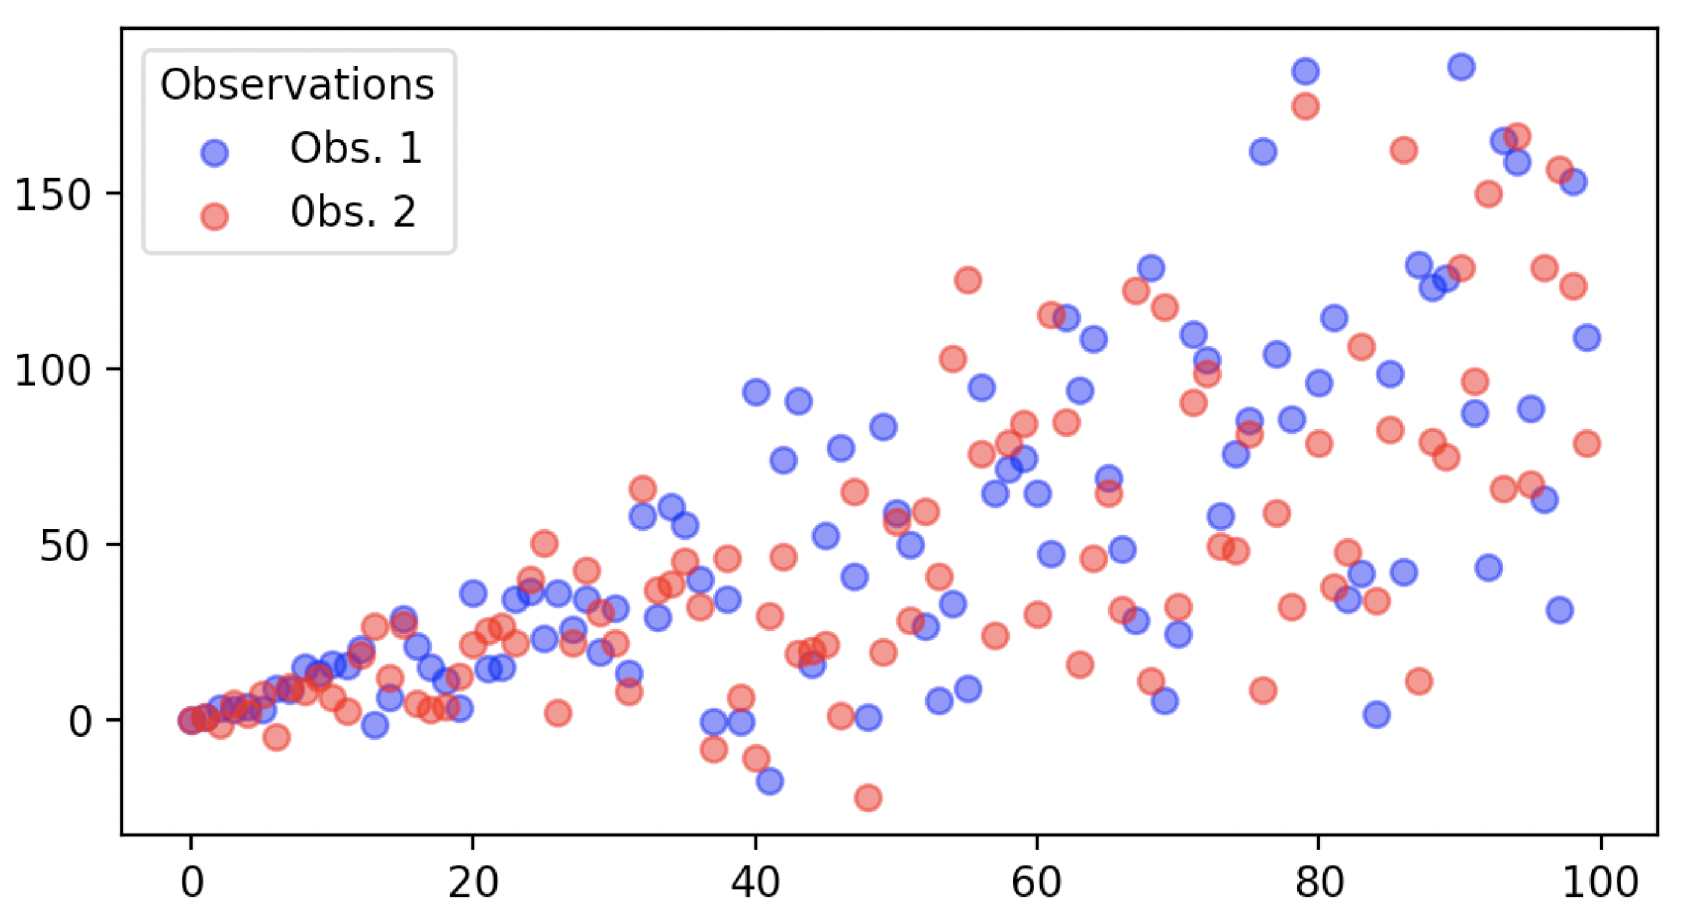
\includegraphics[width=\textwidth]{\dir/two_observations.png}
\caption{Two realizations $X'$ and $X''$ of $\mathfrak{X}$, with $n = 100$. The $x$-axis indicates the indices $\{0, 1, \ldots, n-1\}$ and the $y$-axis indicates the values $X_0, X_1, \ldots, X_{n-1}$, for $X \in \{X', X''\}$.}
\label{fig:illustration_random_array}
\end{figure}

\subsection{What happens if we use statistical learning to solve this problem?}

Statistical learning proposes to train models via \emph{empirical risk minimization (ERM)}. In ERM, we define an instance space $\mathcal{X}$, a hypothesis class $\mathcal{C}$, and a cost function $R$. 

ERM trains a model in $c \in \mathcal{C}$ that minimizes \emph{the expected cost} $\mathbb{E}_X[R(c, X)]$, where $X$ is a random observation of the phenomenon. However, this requires the distribution $p$ behind the phenomenon, which we assume to be unavailable. In consequence, statistical learning advocates to approximate this expected cost with the \emph{empirical cost} $\frac{1}{n} \sum_{i \leq n} R(c, X_i)$, where $X_1, \ldots, X_n$ is a sample of $p$.\looseness=-1

We define the \emph{empirical risk minimizer} as a model $\hat{c}$ that minimizes the empirical cost. That is,
%
\begin{equation}
\hat{c} = \argmin_{c \in \mathcal{C}} \sum_{i \leq n} R(c, X_i).
\end{equation}
%
We assume for simplicity that $\hat{c}$ always exist, although this is not true in general.

If we follow ERM, then we would estimate $i^*$ with $\hat{i} := \argmin_{i \leq n} X'_i + X''_i.$
That is, the index where the minimum of $X' + X''$ is. However, this approach fails in probability as $n$ increases. This is because, with high probability, there is some $i > 0$ for which $X'_i + X''_i < X'_0 + X''_0$.

\subsection{What happens if we do ME+PA?}

ME+PA correctly estimates $i^*$ much more often than ERM. To demonstrate this, we set $n = 100$ and conducted an experiment where we drew at random 100 pairs $(X', X'')$ of independent observations from $\mathfrak{X}$'s distribution. For each pair, we executed ERM and ME+PA to estimate $i^*$. We counted how often each value $i \leq n$ was chosen as the estimate by each method. Figures~\ref{fig:erm_array} and~\ref{fig:mepa_array} demonstrate that in more than 70\% of the cases, ME+PA selects $i^*$ as the estimate, whereas ERM selects it in less than 10\% of the cases.

\begin{figure}
\centering
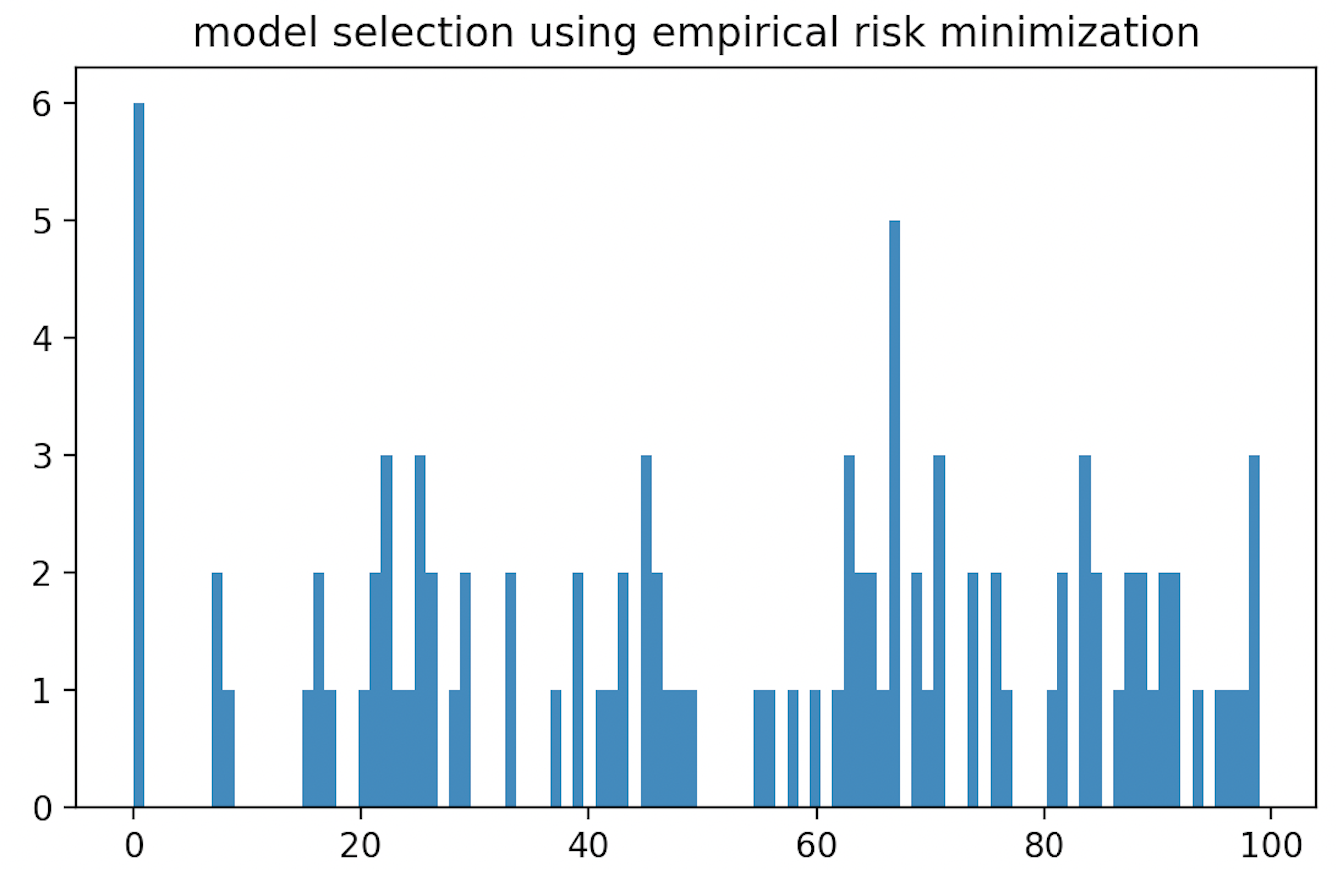
\includegraphics[width=0.8\textwidth]{\dir/erm_array.png}
\caption{Histogram counting how often each estimate in \{0, \ldots, 99\} was picked by ERM as the estimate for $i^*$ across 100 trials. Observe that ERM picks the correct solution less than 10\% of the time.}
\label{fig:erm_array}
\end{figure}

\begin{figure}
\centering
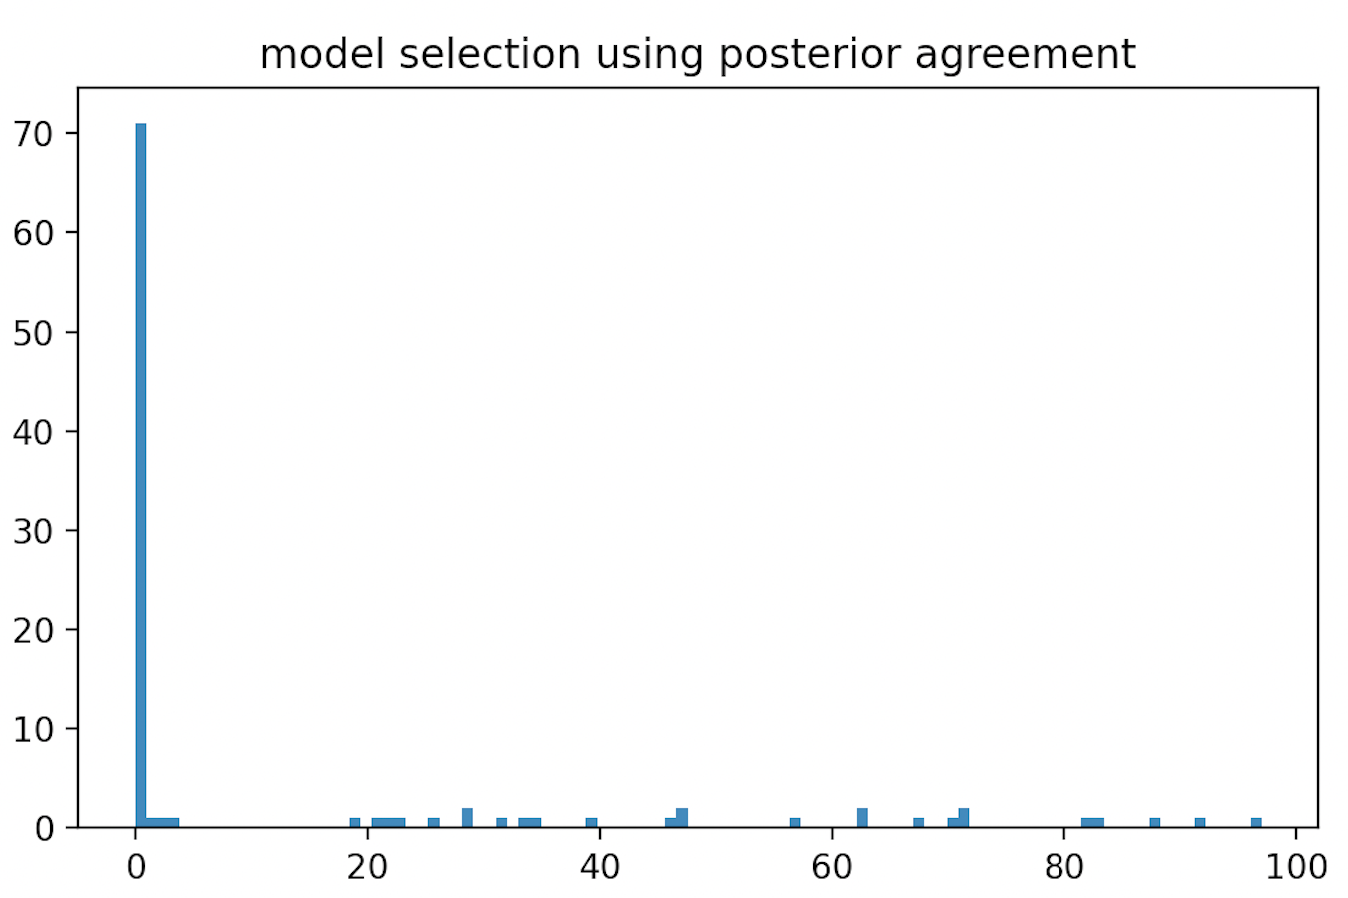
\includegraphics[width=0.8\textwidth]{\dir/mepa_array.png}
\caption{Histogram counting how often each estimate in \{0, \ldots, 99\} was picked by ME+PA as the estimate for $i^*$ across 100 trials. In contrast to ERM, ME+PA picks the correct solution more than 70\% of the time.}
\label{fig:mepa_array}
\end{figure}

\subsection{Application of ME+PA}

We now illustrate the steps to apply ME+PA to this problem.

First, the hypothesis class is $\mathcal{C} = \{0, \ldots, n-1\}$ and the set $\mathcal{X}$ is $\mathbb{R}^n$.

Let $X \in \mathcal{X}$ be an observation. The cost function is $R(c, X) = X_c$. The Gibbs distribution is given by $p(c \mid X) \propto \exp\left(-\frac{1}{T} X_c\right)$. 
%For the two given observations $X'$ and $X''$, a combined Gibbs distribution is $p(c \mid X', X'') \propto \exp\left(-1/T \left(X'_c + X''_c\right)\right)$.

We now need to define a value for $T$. We guess a set of candidate values and, for each of them, we compute the posterior agreement kernel $\kappa(X', X'')$. We then pick the value that yielded the maximum posterior agreement kernel. Finally, we just choose the $\hat{c}$ with largest $p(\hat{c} \mid X')p(\hat{c} \mid X'')$.

\section{Conclusion}

A popular statistical learning approach for training models is empirical risk minimization (ERM). In this approach, you define a cost function and aim for a model that minimizes the expected cost. In most practical cases, minimizing this expected cost is not possible as we do not have access to the distribution governing that expectation. Instead, we approximate it with an empirical estimate, and then compute the model that minimizes this empirical estimate. This chapter questions this approach in two ways. 

\paragraph{ERM trains suboptimal models:} First, in many practical cases, the cost function is non-convex and has several local minima, as in the case of the $K$-means cost function or cost functions used for training neural networks. As a result, empirical risk minimization produces only one model that is a local minimum of the cost function. We argue that such models may be undesirable, as we observed in the $K$-means algorithm. 

\paragraph{Lack of information:} ERM produces only single models. These single models may not give a proper overview of the nature of the phenomenon and may be misleading, as we observed in the random array problem.

\vspace{15pt}

To address these limitations, we present a new approach: maximum entropy and posterior agreement. In maximum entropy, rather than producing a single model, we produce a maximum-entropy distribution over models. This distribution is produced in a way that models with low cost get more mass than models with high cost. The distribution offers then a better overview of the landscape of models that fit the phenomenon. These distributions require a value for a hyper-parameter, called the temperature. This parameter can be chosen using standard model selection techniques. In our case, we propose an alternative, called posterior agreement.

Maximum entropy offers two benefits that we illustrate throughout this script. First, it computes a distribution over models that allows to discriminate between good and bad models. Second, this approach can be applied to many different problems, as mentioned in the publications at the beginning of this chapter. We hope that this script convinces the reader of the potential of maximum entropy for statistical learning.

\renewcommand{\dir}{simulated_annealing}
\chapter{Simulated annealing and methods for exploring Gibbs distributions}
\chaptermark{Simulated annealing}

Let $\mathcal{C}$ and $\mathcal{X}$ be a hypothesis class and an instance space, respectively. Let
also $R$ be a cost function. We are interested in the distribution $p(\cdot \mid X)$,
for a given $X \in \mathcal{X}$. In practice, however, the complexity of $R$ makes often
$p(\cdot \mid X)$ \emph{analytically intractable}: there is no known analytical technique to
use $p(\cdot \mid X)$ to make predictions. In other cases, the size of $\mathcal{C}$ is so large that
computing the normalization constant of this distribution \emph{computationally
intractable}: there is no known efficient algorithm for computing the value
of $p(c \mid X)$, for every $c \in \mathcal{C}$.

This chapter explores methods for computationally handling and eventually
extracting useful models from $p(\cdot \mid X)$, all of them based in sampling.
These methods were originally proposed for optimization, but we use them
here to produce samples of $p(\cdot \mid X)$ that are concentrated around a local
minimum of $R(\cdot, X)$. Moreover, in the case of a particular technique called \emph{simulated annealing}, it has
been formally demonstrated that when its hyper-parameters are adjusted
properly, the samples concentrate around a global minimum of $R(\cdot, X)$.

\section{Chapter overview}

We have seen how the Gibbs distribution concentrates on the global minima
of $R(\cdot, X)$ as the temperature converges to zero. This is advantageous over
ERM methods, as it gives us more candidate models aside from the empirical
risk minimizer that not only have a lower cost but can also generalize
better. Unfortunately, in practice, this Gibbs distribution is intractable,
mainly because of its normalization constant.

One way to go around this intractability is via sampling. There are
methods for sampling intractable distributions that are effective and popular.
We show how to use sampling to explore the Gibbs distribution and
choose models from it.

A popular method to sample intractable distributions is by MCMC
sampling, which we study in Section~\ref{sec:mcmc}. However, MCMC is impractical
for sampling Gibbs distributions. We will see in Section~\ref{sec:mcmc_traversal} that the lower
the temperature of the Gibbs distribution, the more time MCMC requires
to produce a useful sample, as consecutive samples tend to accumulate in
the neighborhood of a local minima of the cost function. We will also see
that when the temperature is high MCMC works well. Unfortunately, in
this case the Gibbs distribution does not substantially discriminate between
good and bad models.

We study simulated annealing (SA) in Section~\ref{sec:simulated_annealing} and see how it overcomes
this limitation of MCMC \emph{by decreasing the temperature during the
MCMC sampling}. SA starts by setting the temperature to a very large
value, so that the Gibbs distribution is almost uniform and MCMC efficiently produces samples. After some samples, SA alternates between decreasing
the current temperature and drawing more samples. We will see,
albeit informally, that the alternation between sampling and temperature
decreasing avoids that SA gets stuck in the neighborhood of a bad local
minimum. It can be formally proven that when the temperature decreasing
schedule is done properly, SA converges to the cost function's global
minimum.

Simulated annealing offers two advantages over the standard empirical
risk minimization (ERM). First, it can converge to a global minimum, or
at least to a local minimum of good quality. Second, the sampling nature
of SA gives not only one but several models to choose from. In contrast,
ERM tends to produce only one model that is just local minima of the
cost function. As seen in the random array problem from Section 1.4, this
model may not generalize well.

In the case of clustering, the stochastic nature of SA makes it superior
to ERM methods like K-means, as we will study in Chapter 3. Moreover,
we will see that in several instances, SA can be improved to a more exact
and simpler method, called \emph{deterministic annealing} (DA).

\section{Sampling as a way to extract models from Gibbs distributions}
\label{sec:sampling}

In many interesting cases in practice, $p(\cdot \mid X)$ is intractable. However, there
are effective methods for sampling intractable distributions. Sampling gives
us a way to explore and to choose a model from $p(\cdot \mid X)$, when $\mathcal{C}$ is a vector
space, or at least a space that admits a notion of an average: draw a sample from $p(\cdot \mid X)$ and then propose the average of that sample as a model.
Figure~\ref{fig:two_observations_sa} illustrates two observations from the random array problem
from Section~\ref{sec:random_array}. Here, the array has length 100. The upper graphic in Figure~\ref{fig:means_pas_two_arrays} illustrates the mean of the two Gibbs distributions induced by
$R(\cdot, X')$ and $R(\cdot, X'')$ as a function of the temperature. Observe that in
this case, the mean would then be the model that we would choose, if we
could only access $p(\cdot \mid X')$ or $p(\cdot \mid X'')$ via sampling. The lower graphic in Figure~\ref{fig:means_pas_two_arrays}
illustrates the kernel posterior agreement between the two observations as
a function of the temperature.

\begin{figure}[hbtp]
\centering
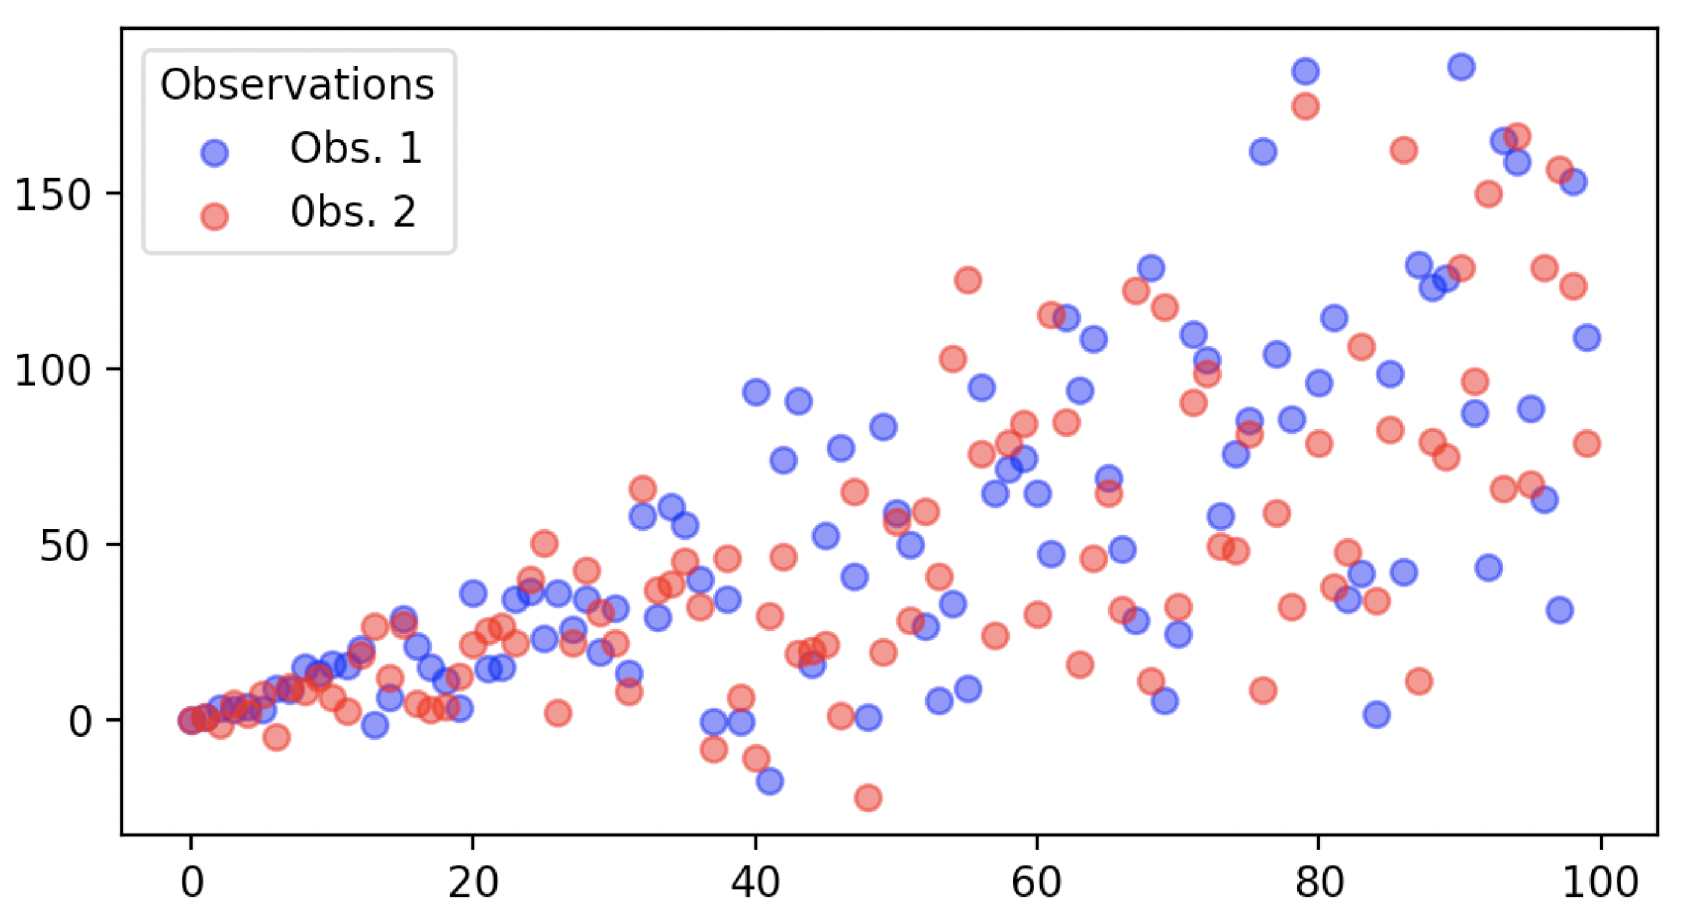
\includegraphics[width=\textwidth]{\dir/two_observations}
\caption{}
\label{fig:two_observations_sa}
\end{figure}

\begin{figure}[hbtp]
\centering
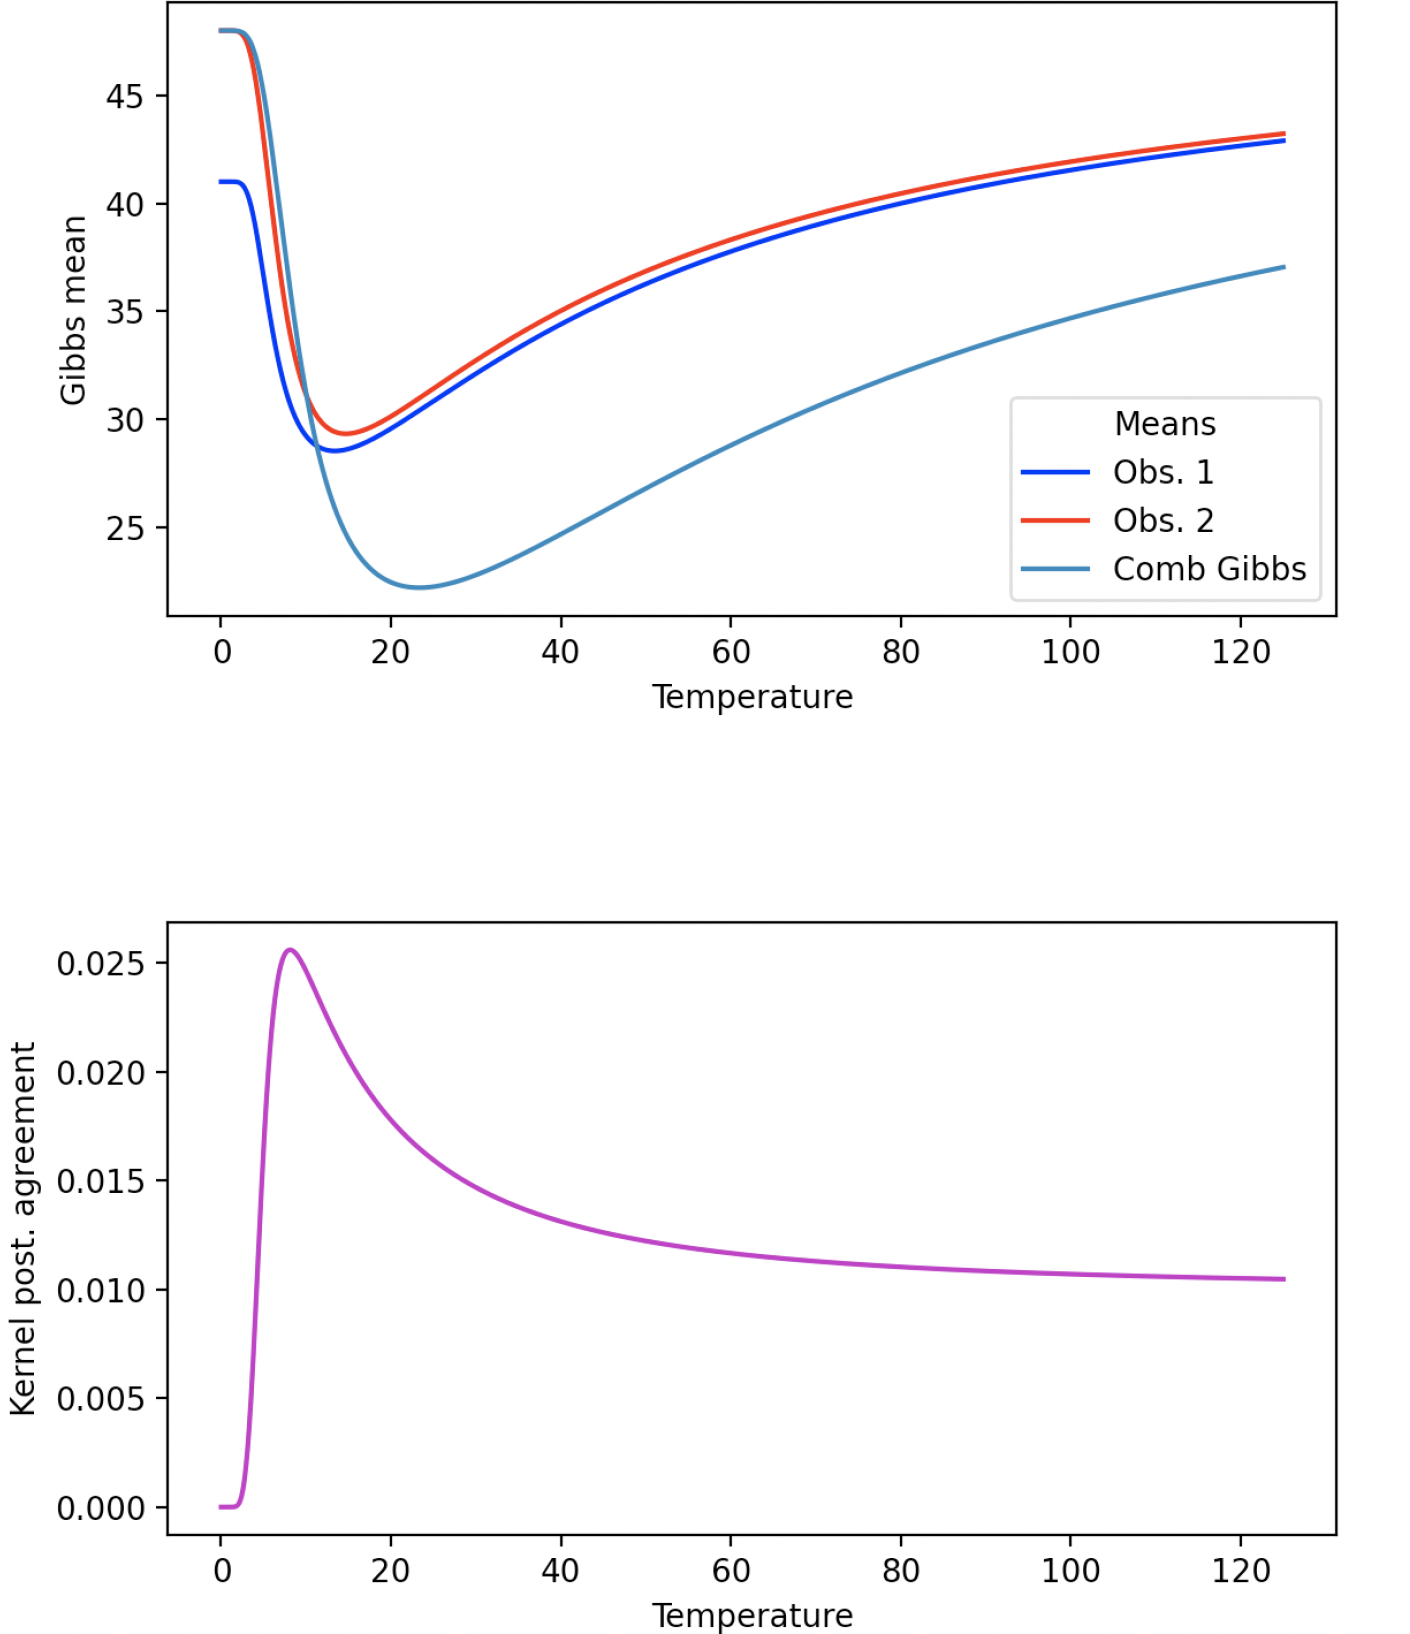
\includegraphics[width=\textwidth]{\dir/means_pas_two_arrays}
\caption{}
\label{fig:means_pas_two_arrays}
\end{figure}

As $T \to \infty$, the mean of the two Gibbs distributions lie near to 50. This
is because at a sufficiently high temperature, the Gibbs distributions look
like uniform distributions. As the temperatures start decreasing, the distributions
concentrate more and more on the array entries with the lowest
values. Such values are in the first half of the array. This is why the means
decrease as the temperature decreases from 120 to 20 for the two Gibbs
distributions. However, the means start increasing when the temperature
gets below 20. This is because the Gibbs distributions start concentrating
on the arrays' minima. In particular, when the temperature approaches
zero, the distributions concentrate almost entirely on the minima of the
corresponding arrays. The combined Gibbs distribution has a similar behavior.

When searching for a good model in the Gibbs distribution, it is important
to choose an adequate value of the temperature. We argue that
such a value can be computed by maximizing the kernel posterior agreement
between two given observations. Observe in the lower graphic of
Figure~\ref{fig:means_pas_two_arrays} that the temperature at which the kernel posterior agreement is
maximum is very close to the temperature at which the means of the two Gibbs distributions are minimized.


\section{MCMC sampling}
\label{sec:mcmc}

MCMC sampling is one of the most popular methods for sampling from
intractable distributions, especially when the source of intractability is the
normalization constant. We give here a basic recap of MCMC. For a more
thorough overview, please refer to Bishop's ``Pattern recognition and machine
learning'' or Murphy's ``Machine learning: a probabilistic perspective''.

\subsection{Markov chain Monte Carlo}

Given a distribution $p$, MCMC sampling is usually done by defining a
parameterized family of conditional \emph{transition distributions} $\pi(\cdot \mid c)$, for an
arbitrary $c \in \mathcal{C}$. This distribution gives rise to a graph $G$ whose vertices
are $\mathcal{C}$ and where there is an edge between any two $c, c' \in \mathcal{C}$ iff $\pi(c' \mid c) > 0$.
MCMC sampling then proceeds to produce samples iteratively as follows.
First, pick an arbitrary $C_0 \in \mathcal{C}$. Then for $t = 1, 2, \ldots$, sample $C_t$ from $\pi\left(\cdot \mid C_{t-1}\right)$. The samples eventually look like samples from $p$ if the conditions
below are met.

\begin{theorem}
Let $p$ be a distribution over $\mathcal{C}$ and let $\{\pi(\cdot \mid c)\}_{c \in \mathcal{C}}$ be a parameterized
family of conditional distributions on $\mathcal{C}$ meeting the following
requirements.

\begin{itemize}
\item $G_\pi$ is connected.
\item There is an edge from a vertex to itself in $G_\pi$.
\item $\pi(c' \mid c)p(c) = \pi(c \mid c')p(c')$, for any two $c, c' \in \mathcal{C}$.
\end{itemize}

Let $C_0, C_1, \ldots$ be a sequence of random variables such that, for $1 \leq t$,
$C_t$'s distribution is given by $\pi(\cdot \mid C_{t-1})$. Then, for $c \in \mathcal{C}$,
%
\begin{equation}
\lim_{t \to \infty} \prob\left(C_t = c\right) = p(c).
\end{equation}
%
\label{thm:convergence_markov}
\end{theorem}

The proof is found in standard probability textbooks and is studied in
the course \emph{probabilistic artificial intelligence}.

\subsection{The Metropolis-Hastings trick}

MCMC gives a simpler recipe to sample an intractable distribution $p$: just
come up with a transition distribution fulfilling the three requirements
from Theorem~\ref{thm:convergence_markov}. The hardest requirement is the last one, called detailed
balance, as it demands a good understanding of $p$ in order to fulfil that
equation. Fortunately, there is a convenient trick proposed by Metropolis
and Hastings that easily yields such a transition distribution.

The trick works for distributions where the intractability comes from
the normalization constant, which is often the case in Bayesian methods
and in our Gibbs distributions. So let us assume that $p(c) \propto f(c)$, where
$f(c)$ is tractable. The trick consists of two steps:

\begin{enumerate}
\item Define a parameterized family of conditional proposal distributions
$\{q(\cdot \mid c) \mid c \in \mathcal{C}\}$ such that $G_q$ is connected and every vertex in $G_q$
has an edge to itself.
\item Define, for $c, c' \in \mathcal{C}$, the \emph{accepting probability}
%
\begin{equation}
A(c', c) := \min\left\{1, \frac{q(c \mid c')p(c')}{q(c' \mid c)p(c)}\right\} = \min\left\{1, \frac{q(c \mid c')f(c')}{q(c' \mid c)f(c)}\right\}.
\end{equation}
%
\end{enumerate}

\begin{exercise}
Let $c \in \mathcal{C}$ and
%
\begin{equation}
\pi(c' \mid c) := \begin{cases}
q(c' \mid c)A(c', c) & \text{if $c \neq c'$ and}\\
1 - \sum_{c' \neq c}q(c' \mid c)A(c', c) & \text{otherwise}.
\end{cases}
\end{equation}
%
Show that $\pi(\cdot \mid c)$ fulfils the requirements from Theorem 1.
\end{exercise}

\begin{exercise}
In our context, we usually choose proposal distributions $q(\cdot \mid \cdot)$
that are symmetric. That is, $q(c' \mid c) = q(c \mid c')$ for $c, c' \in \mathcal{C}$. Show that,
in this case, the Metropolis-Hastings transition distribution $\pi(\cdot \mid c)$ for a
Gibbs distribution $p(c \mid X) \propto \exp\left(-\frac{1}{T}R(c, X)\right)$ simplifies to the following:

\begin{itemize}
\item If $c \neq c'$ and $R(c', X) > R(c, X)$, then $\pi(c' \mid c) = q(c' \mid c)\rho(c, c')$, where $\rho(c, c') = \exp\left(\frac{1}{T}\left(R(c, X) - R(c', X)\right)\right)$.
\item Otherwise, if $c \neq c'$ and $R(c', X) \leq R(c, X)$, then $\pi(c' \mid c) = q(c' \mid c)$.
\item Otherwise,
%
\begin{equation}
\pi(c' \mid c) = 1 - \sum_{c' : R(c', X) \leq R(c, X)}q(c' \mid c) - \sum_{c': R(c', X) > R(c, X)}q(c' \mid c)\rho(c, c').
\end{equation}
%
\end{itemize}
\end{exercise}

For $c \in \mathcal{C}$, we can then draw a sample $C$ from $\pi(\cdot \mid c)$ in two easy steps:

\begin{enumerate}
\item Draw a sample $\tilde{C}$ from $q(\cdot \mid c)$.
\item If $R(\tilde{C}, X) > R(c, X)$, then draw a sample $b$ from a Bernoulli distribution with mean $\exp\left(\frac{1}{T}\left(R(c) - R(\tilde{C})\right)\right)$. If $b = 1$, then $C:= \tilde{C}$. Otherwise, $C := c$.
\end{enumerate}

\subsection{MCMC sampling of Gibbs distributions}

We now summarize all our insights so far. Assume given a Gibbs distribution $p(c \mid X) \propto \exp\left(-\frac{1}{T}R(c, X)\right)$. The normalization constant
$\sum_{c} \exp\left(-\frac{1}{T}R(c, X)\right)$,
also called \emph{the partition function}, is intractable in most of the interesting
cases. We are interested in models that have a high probability mass according
to this distribution, as we believe that some of them generalize
very well. To retrieve these models without dealing with the intractability
of $p(c \mid X)$, we do the following.

\begin{enumerate}
\item Define a symmetric proposal distribution $q(\cdot \mid c)$ such that $G_1$ is
connected and every vertex in $G_q$ has an edge to itself.
\item Let $C_0$ be an arbitrary element in $C$.
\item For $t = 1, 2, \ldots$, draw a sample $C_t$ from $\pi(\cdot \mid C_{t-1})$as explained
above.
\end{enumerate}

By Theorem~\ref{thm:convergence_markov}, the samples produced by this algorithm eventually become
samples of $p(\cdot \mid X)$.

It is important to emphasize that MCMC and the Metropolis-Hastings
trick are not restricted only to Gibbs distributions. These sampling techniques
have existed for decades and are still very popular today for dealing
with intractable distributions.

\section{MCMC sampling as a randomized traversal algorithm}
\label{sec:mcmc_traversal}

Before we continue, we give a toy example that gives us some intuitions
of how MCMC sampling works for Gibbs distributions. We argue that
MCMC sampling of $p(\cdot \mid X)$ can be understood with a parable of a treasure
hunter that explores the hypothesis class $\mathcal{C}$ in a random way, searching
for local minima of $R(\cdot, X)$. The sequence of locations visited by the hunter
correspond to the sequence of samples drawn via MCMC. When the temperature
is low, this hunter lingers in local minima of $R(\cdot, X)$ that are close
to the hunter's starting position. When the temperature is high, the hunter
roams over $\mathcal{C}$, showing little preference over the different local minima of $R(\cdot, X)$.

In the next section, we explain why this is problematic in practice: for
the Gibbs distribution to be useful for us, it must have a sufficiently low
temperature so that its probability mass is concentrated on valuable local
minima of $R(\cdot, X)$. However, such a low temperature prevents MCMC to
leave bad local minima and makes the success of MCMC very sensitive to
the choice of the intial sample, making MCMC impractical for our analyzing
Gibbs distributions. Afterwards, we show how simulated annealing solves
this issue.

\subsection{Illustrative example}

Let $C = \{0, 1, \ldots, 24\}$ and consider the cost function $R(\cdot, X)$ in Figure~\ref{fig:chainsaw_sa},
where $X$ is some arbitrary observation. The horizontal axis describes the
models in $\mathcal{C}$. The vertical axis denotes $R(c, X)$, for some $c \in \mathcal{C}$. Notice
that the minimizer of $R(\cdot, X)$ is $c^* = 19$.

\begin{figure}
\centering
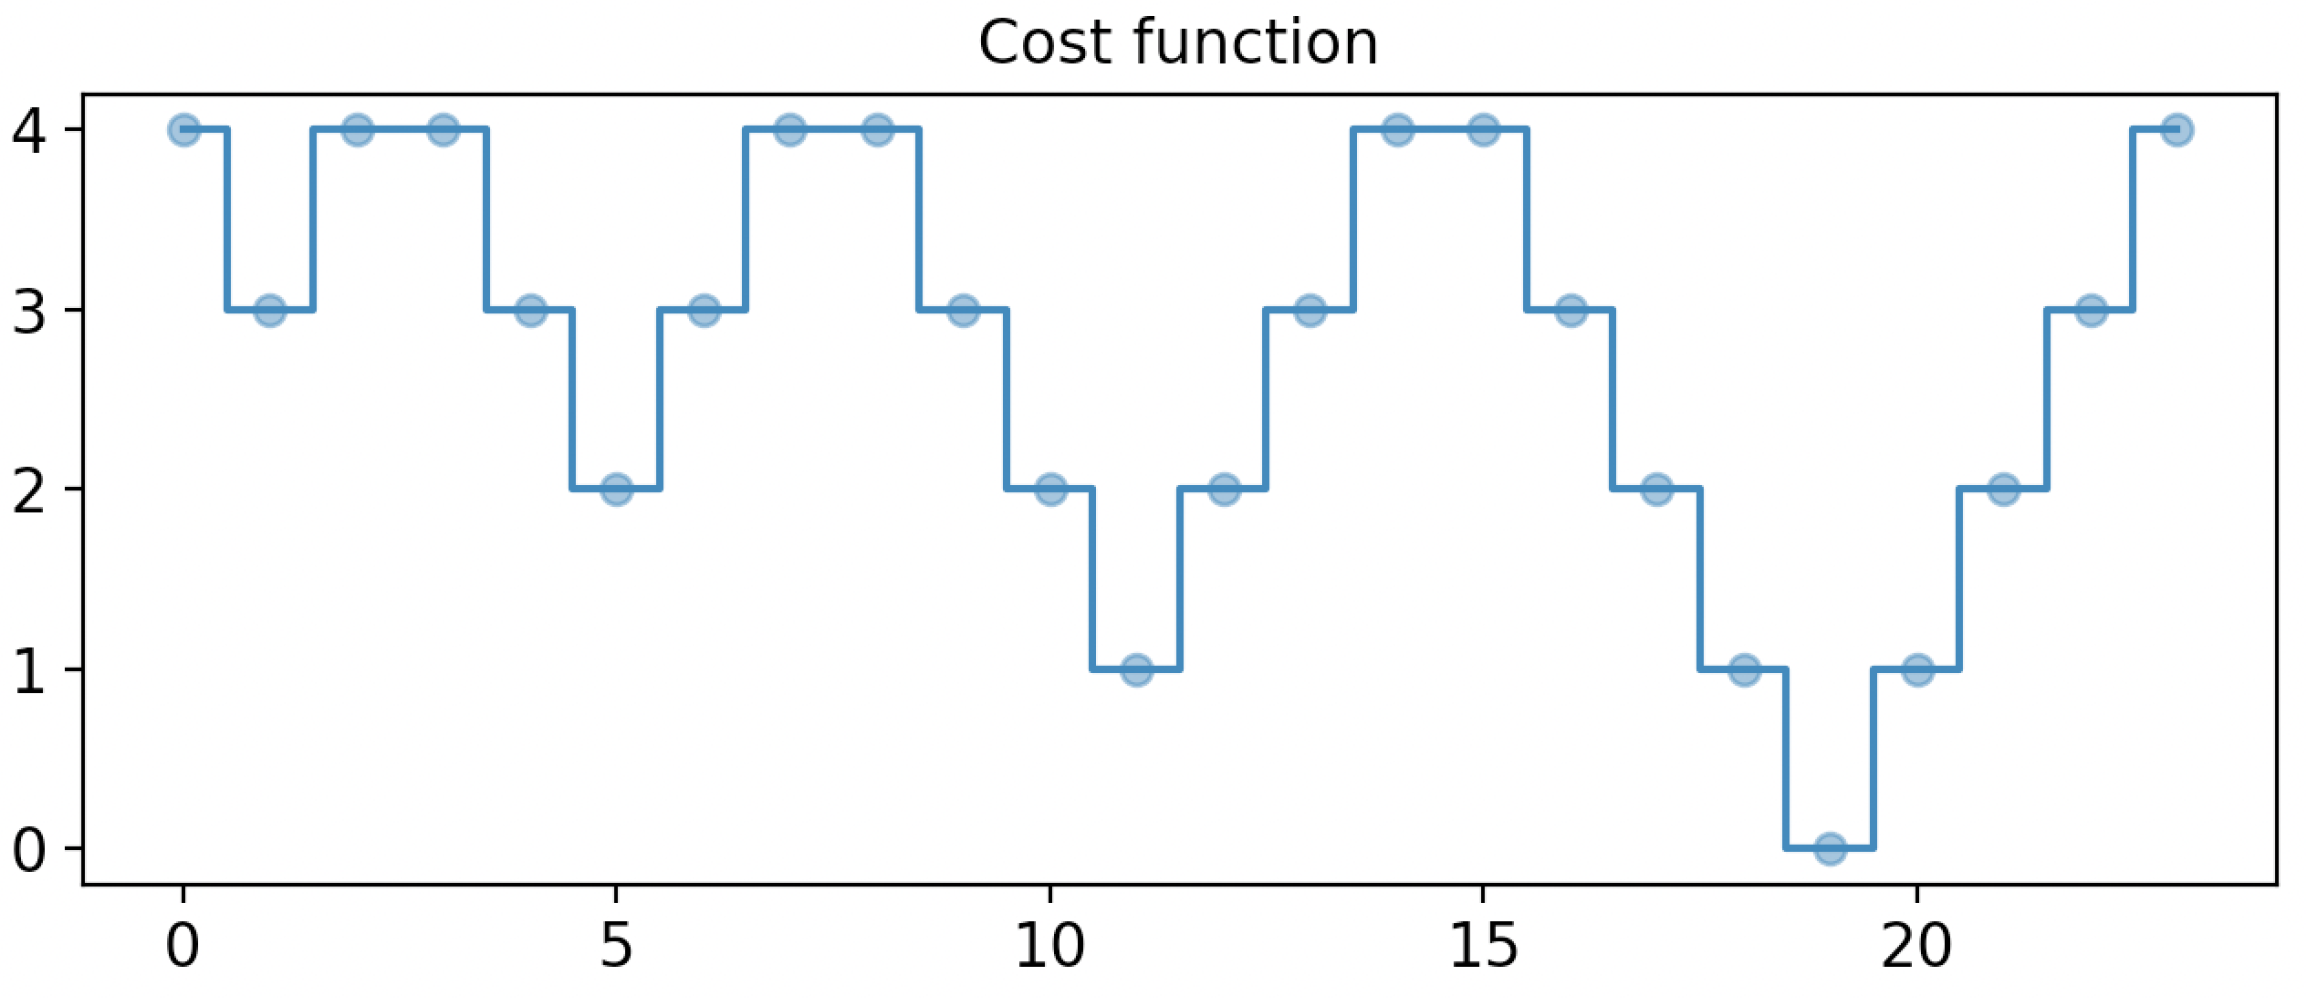
\includegraphics[width=\textwidth]{\dir/chainsaw}
\caption{}
\label{fig:chainsaw_sa}
\end{figure}

Figures~\ref{fig:mcmc_high_temp}--\ref{fig:mcmc_low_temp} depict four Gibbs distributions over $\mathcal{C}$ with different
temperatures. Observe that the higher the temperature, the more uniform
the Gibbs distribution is. In contrast, the lower the temperature, the more
concentrated on $c^*$ the distributions is.

\begin{figure}
    \centering
    \begin{subfigure}[b]{0.6\textwidth}
        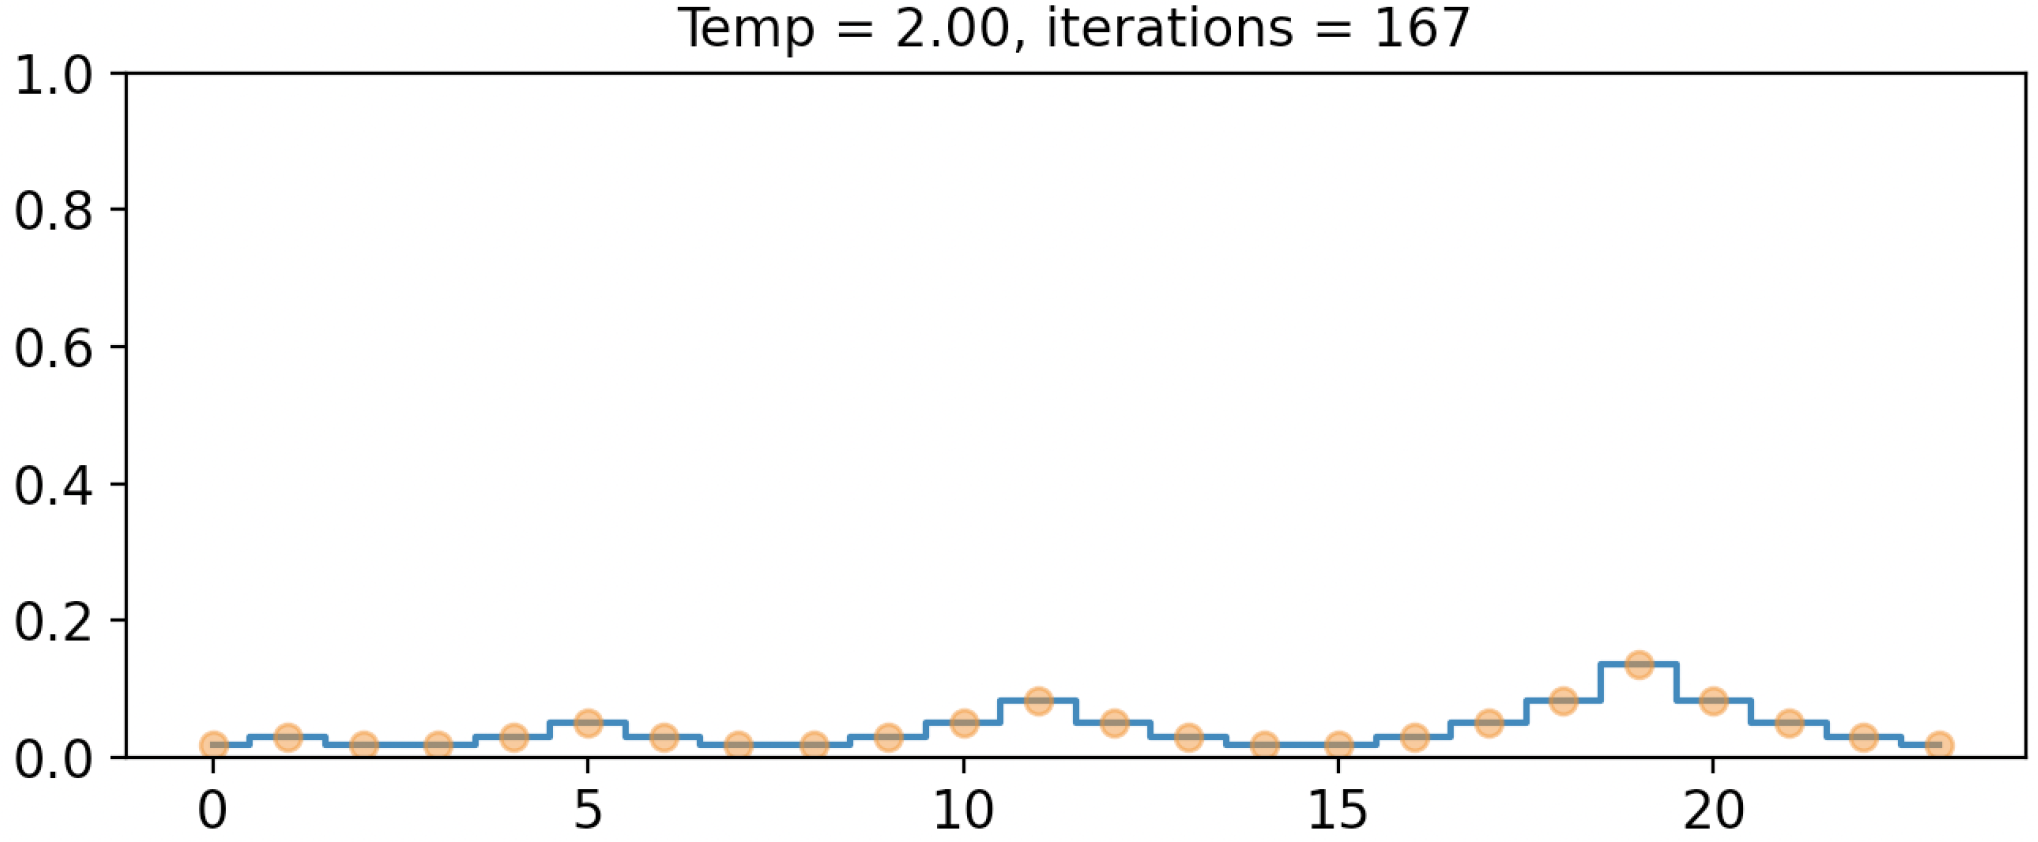
\includegraphics[width=\textwidth]{\dir/mcmc_high_temp}
        \caption{}
        \label{fig:mcmc_high_temp}
    \end{subfigure}

    \begin{subfigure}[b]{0.6\textwidth}
        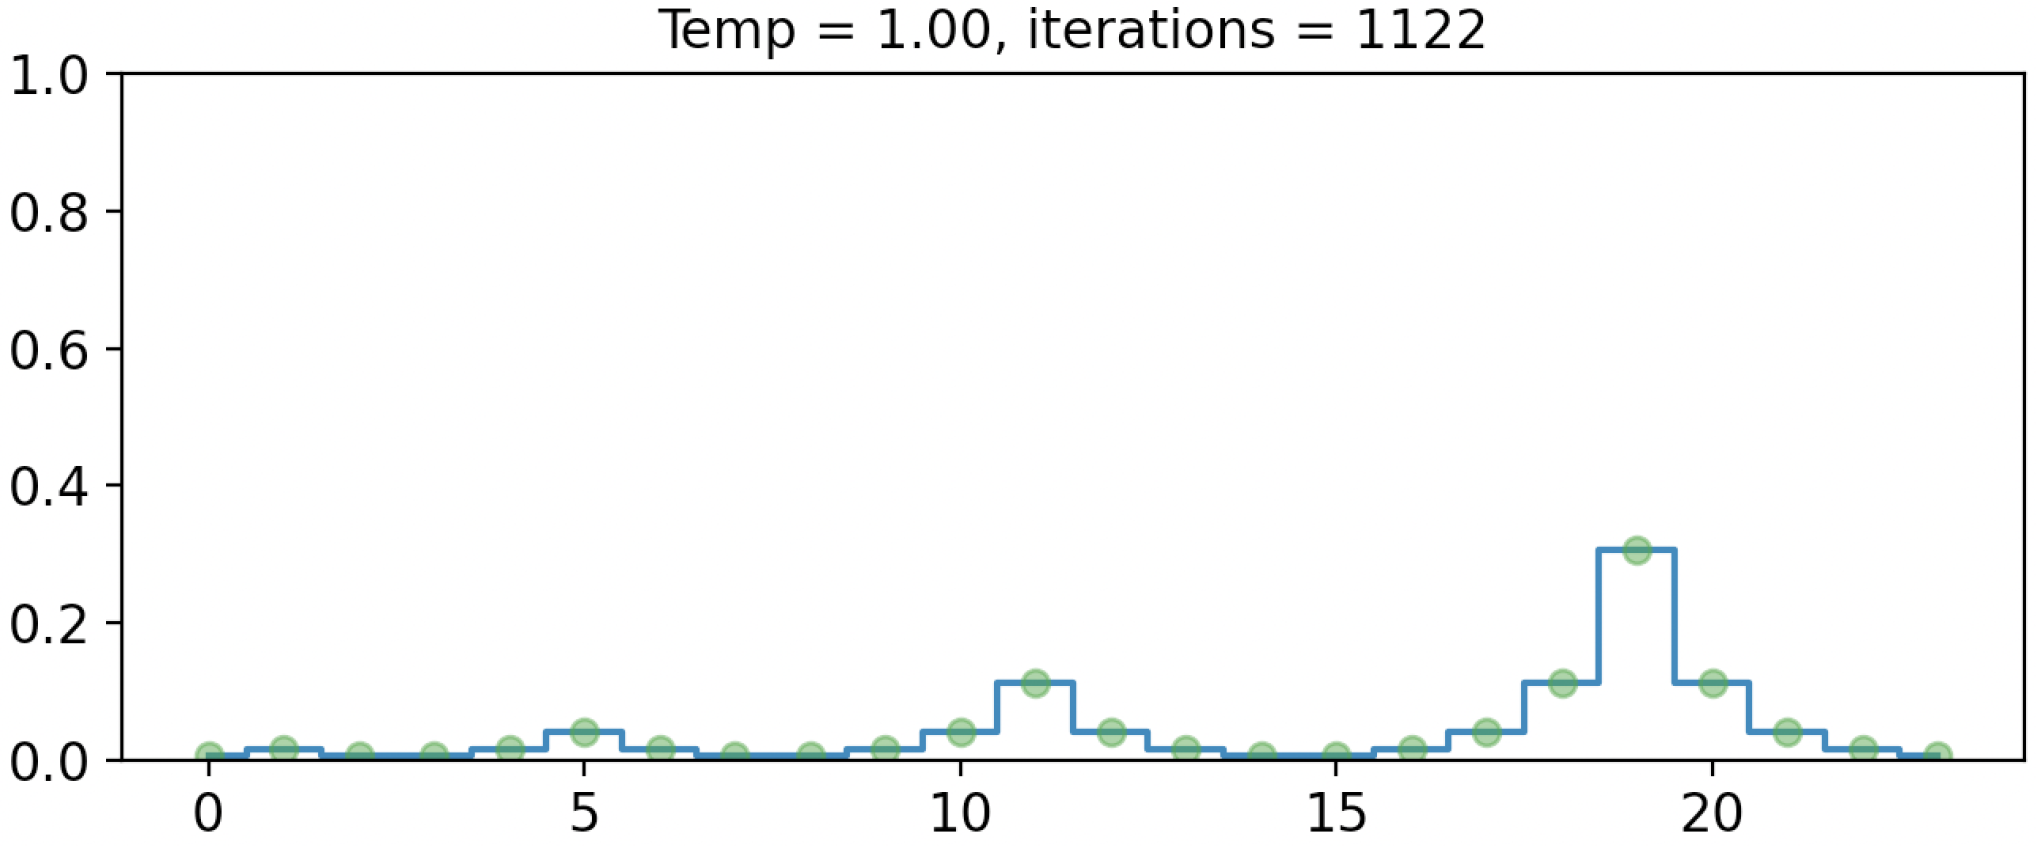
\includegraphics[width=\textwidth]{\dir/mcmc_mid_temp1}
        \caption{}
        \label{fig:mcmc_mid1_temp}
    \end{subfigure}
    
    \begin{subfigure}[b]{0.6\textwidth}
        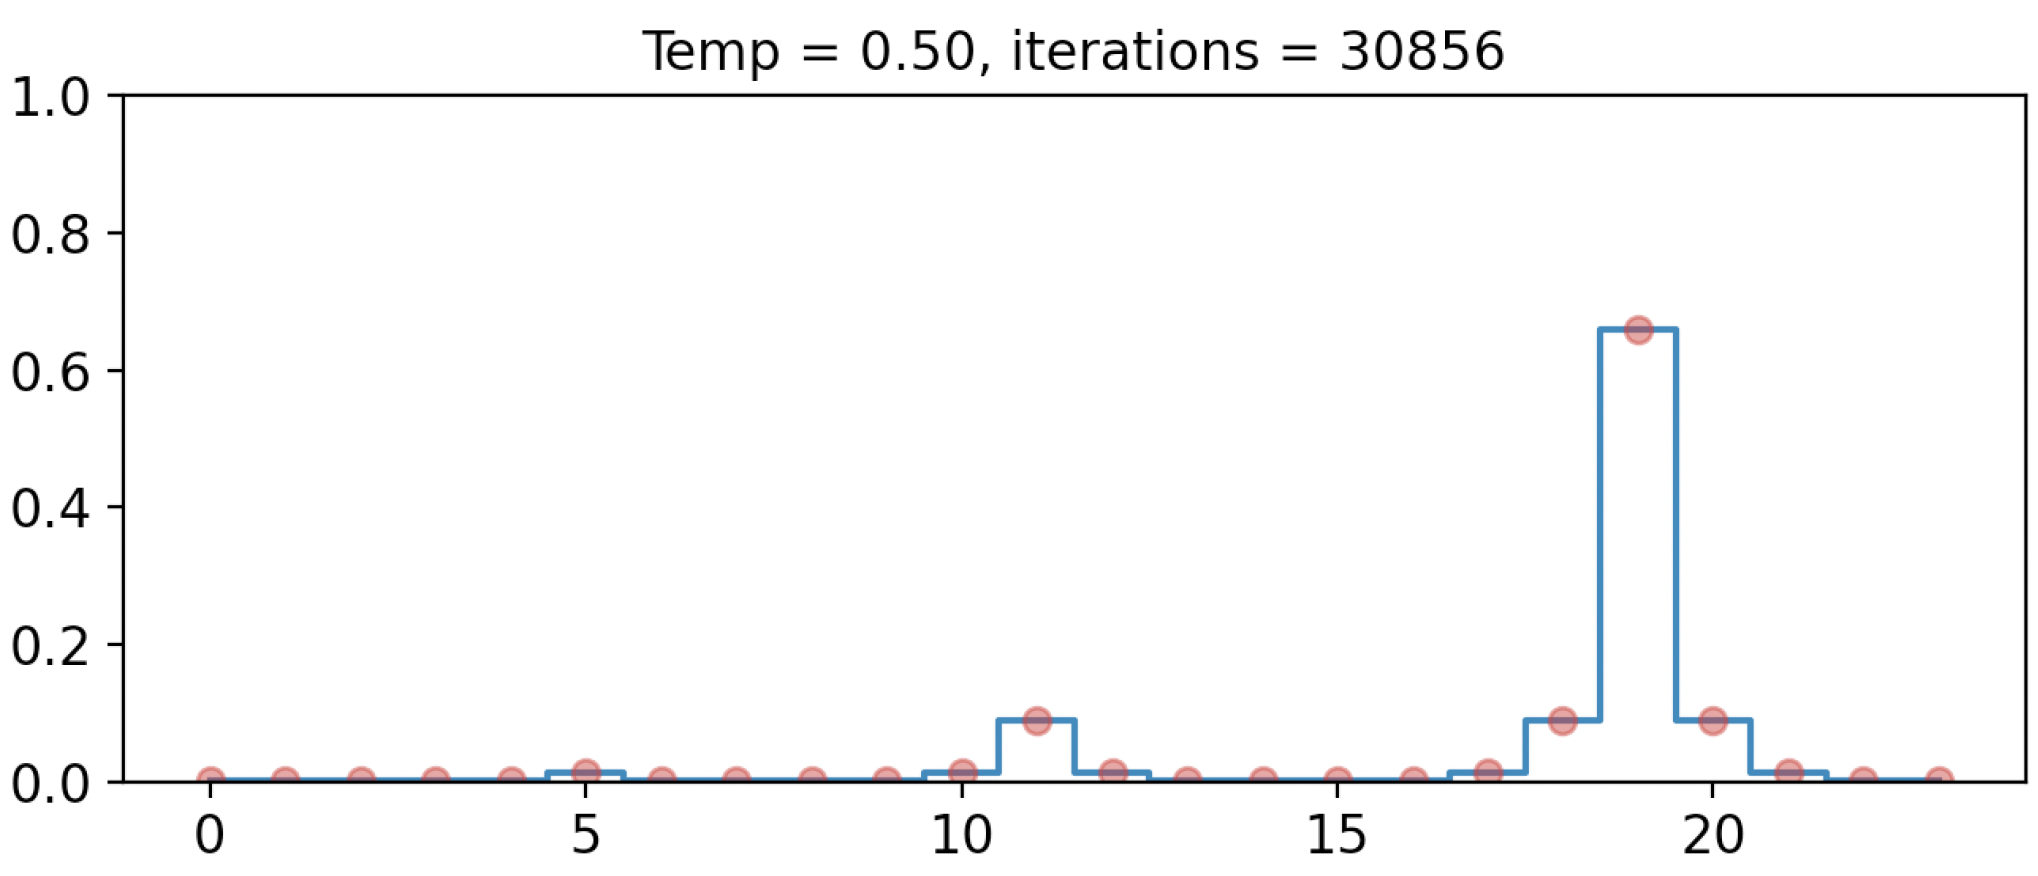
\includegraphics[width=\textwidth]{\dir/mcmc_mid_temp2}
        \caption{}
        \label{fig:mcmc_mid2_temp}
    \end{subfigure}

    \begin{subfigure}[b]{0.6\textwidth}
        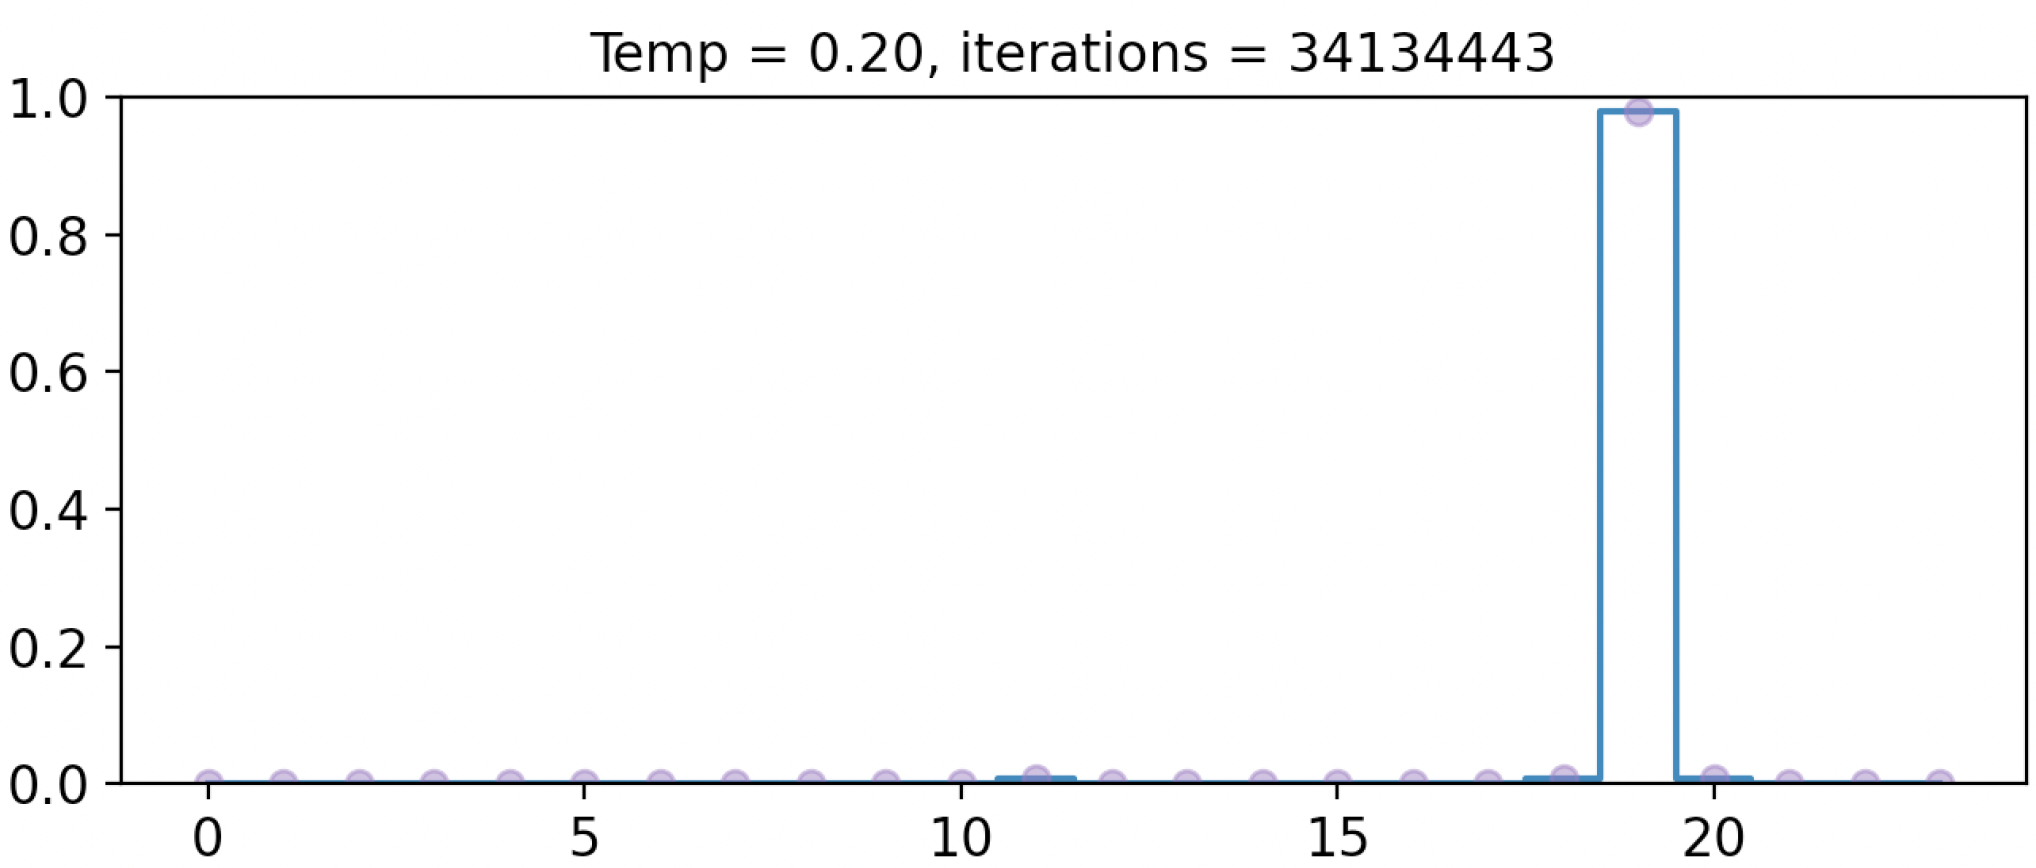
\includegraphics[width=\textwidth]{\dir/mcmc_low_temp}
        \caption{}
        \label{fig:mcmc_low_temp}
    \end{subfigure}
    \caption{Four different Gibbs distributions induced by the cost function
from Figure~\ref{fig:chainsaw_sa}. Observe that the lower the temperature, the more
concentrated the distribution is on the empirical risk minimizer $c^*$. Furthermore,
the number of samples needed to reach $c^*$ from $c_0 = 0$ increases
dramatically as the temperature decreases.}
\end{figure}

\subsection{MCMC as a treasure hunter}

Let us now do MCMC sampling over one of these Gibbs distributions.
We first define a family of proposal $c \in \mathcal{C}$ via
the following randomized algorithm. Assume that you have sampled $c$. To
draw the next sample, flip a coin. If heads comes out, then the next sample
is $c$ again. Otherwise, flip a coin again. If heads comes out, the next sample is $\min(24, c + 1);$ otherwise, it is $\max(0, c - 1)$. More formally,
%
\begin{equation}
q(c' \mid c) =
\begin{cases}
1/4 & \text{if $c' = c + 1$ and $c < 24$},\\
1/4 & \text{if $c' = c + 1$ and $c > 0$},\\
1/2 & \text{if $c' = c$},\\
3/4 & \text{if $c' = c = 0$},\\
3/4 & \text{if $c' = c = 24$}.
\end{cases}
\end{equation}

One can then imagine the MCMC sampling of a Gibbs distribution as a
treasure hunter that randomly traverses the landscape of the cost function
in search for a local minimum of $R(\cdot, X)$. The hunter starts at some location $C_0$. Then it uses the proposal distribution $q(\cdot \mid C_0)$ to choose the location
$C_1$ where it will go next. If $R(C_1, X) \leq R(C_0, X)$, the hunter eagerly
moves to that location. Otherwise, the hunter ponders whether to risk
forgoing the current location, with the hopes that moving to this higher cost
location leads to a location better than the current one. The pondering
is simulated by drawing a sample $B$ from a Bernoulli distribution with
mean $\exp\left(\frac{1}{T}\left(R(C_0, X) - R(C_1, X)\right)\right)$. Observe that the higher $R(C_1, X)$
is with respect to $R(C_0, X)$, the less motivated is the hunter to move to
that location. This motivation is also affected by the temperature. The
lower the temperature, the less motivated is the hunter to move to locations
higher than the current one.

\subsection{The tradeoff induced by the temperature}

Equipped with the intuition of the MCMC sampling algorithm as a treasure
hunter, we report in Figures~\ref{fig:mcmc_high_temp}--\ref{fig:mcmc_low_temp} the number of samples that
we need to draw via MCMC sampling until $c^*$ is sampled for the first time,
when the first sample is $C_0 = 0$. In other words, we report the number
of locations that were visited by the hunter before reaching $c^*$, assuming
that the hunter starts from $C_0 = 0$. Observe that the lower the temperature,
the more samples are needed to draw before sampling $c^*$. This is simply
because in order to reach $c^*$ from $C_0$, the hunter must go through three local
minima before reaching $c^*$. At each local minimum, the hunter must
ponder and choose to forgo the current local minimum. The choice to forgo
becomes more unlikely the more we lower the temperature. This is why
the lower the temperature, the more iterations are needed by the hunter to
reach the $c^*$ for the first time.

The tradeoff induced by the temperature is problematic in practice.
We want a high temperature, so that the hunter is motivated to explore
the landscape of the cost function. However, a high temperature reduces
the ability of the Gibbs distribution to discriminate between good and bad
models because the distribution looks more like a uniform distribution. So
we also want a low temperature, but this negatively affects the hunter's
motivation, making the hunter resistant to leave bad local minima.

\section{Simulated annealing}
\label{sec:simulated_annealing}

Simulated annealing overcomes this tradeoff with a natural solution: start
at a high temperature and then alternate between MCMC sampling and
decreasing the temperature. When the temperature is high, the hunter
roams through the model space. By gradually decreasing the temperature,
we hope that the hunter starts to linger more and more on valuable local
minima. When the temperature becomes significantly low, we hope that
the hunter stays in that local minima. Algorithm~\ref{algo:sa_sa} describes simulated
annealing.

\begin{algorithm}
\begin{algorithmic}[1]
\State Let
\State \quad $\epsilon > 0$ be a temperature threshold.
\State \quad $R(\cdot, X)$ be a cost function,
\State \quad \texttt{reduce} be a function for decreasing the temperature.
\State \quad $q(\cdot \mid c)$, for $c \in \mathcal{C}$, a family of proposal distributions.
\State
\Function{SimAnn}{$\epsilon$, $R(\cdot, X)$, \texttt{reduce}, $\{q(\cdot \mid c) \mid c \in \mathcal{C}\}$}
\State $T \gets \infty$ \Comment{$\infty$ is a sufficiently large value.}
\State $c^T_0 \gets \$$ \Comment{Fix the first element in the sample.}
\While{$T > \epsilon$}
\For{$t = 0\ldots N$}
\State $\tilde{c} \gets \texttt{sample} \; q(\cdot \mid c^T_t)$
\If{$R(\tilde{c}, X) \leq R(c^T_t, X)$}
\State $c^T_{t+1} \gets \tilde{c}$
\Else
\State $b \gets \texttt{sample}$ Bernoulli $\left(\exp\left(\frac{1}{T}\left(R(c^T_t, X)-R(\tilde{c}, X)\right)\right)\right)$
\If{$b = 1$}
\State $c^T_{t+1} \gets \tilde{c}$
\Else
\State $c^T_{t+1} \gets c^T_t$
\EndIf
\EndIf
\EndFor
\State $c_0 \gets c^T_N$ \Comment{Fix the first element for the next sample}
\State $T \gets \texttt{reduce}(T)$
\State $c^T_0 \gets c_0$
\EndWhile
\State \textbf{return} $\left(c^T_t\right)_{T, t}$
\EndFunction
\end{algorithmic}
\caption{Simulated annealing}
\label{algo:sa_sa}
\end{algorithm}

Simulated annealing offers two advantages. First, the gradual temperature
decrease allows the hunter to escape bad local minima, while searching
for the cost function's global minima. So in practice, one can expect that
the cost of simulated annealing's solutions are lower than those from classical
ERM schemes like gradient descent, as they do not have procedures
to escape bad local minima. Second, the sampling nature of simulated annealing
gives us not one but many solutions that are in the ``neighborhood''
of the empirical risk minimizer.

%It is very difficult to diagnose when a Markov chain has burned in.
%Murphy's 24.4.2


\renewcommand{\dir}{deterministic_annealing}
\chapter{Deterministic annealing}

\section{The problem of centroid-based cluster-
ing}
\label{sec:problem}

In this chapter, we consider the problem of centroid-based clustering. In
this problem, an observation is a sample $X = \{x_1, \ldots, x_N\} \subseteq \mathbb{R}^d$ of points
and our objective is to compute a set $\{\theta_1, \ldots, \theta_K\} \subseteq \mathbb{R}^d$ of $K$ centroids and a \emph{cluster assignment} function $c : \{1, \ldots, N\} \to \{1, \ldots, K\}$, where $K \in \mathbb{N}$ is a hyperparameter.
We let the hypothesis class $\mathcal{C}$ be all possible cluster assignment functions with fixed $K$.

As cost function, we choose the $K$-means cost function:
%
\begin{equation}
R(c, \theta, X) := \sum_{i \leq n} \left\|x_i - \theta_{c(i)}\right\|^2.
\label{eq:k_means_cost_fun}
\end{equation}
%
Note that, in contrast to $K$-means, we neither require $\theta_k$ to be the mean of all points in $X$ assigned to cluster $k$ nor that $c(x)$ is the index of the centroid closest to $x$.

\section{Chapter outline}
\label{sec:chapter_outline}

In this chapter, we study how to apply simulated annealing to the problem
of clustering, and derive a simplified version called deterministic annealing, proposed by Kenneth Rose~\cite{rose1998deterministic}. We compare deterministic annealing
against a popular ERM approach, $K$-means, and empirically show that deterministic annealing often provides solutions that generalize better than
$K$-means. Furthermore, combining deterministic annealing with posterior
agreement gives a method to estimate the number of clusters while executing
deterministic annealing.

\subsection*{Deterministic annealing}

Deterministic annealing originates from applying simulated annealing to
clustering. We can summarize simulated annealing in this context in the
following three steps.

\begin{enumerate}
\item Pick a first model $c$ and an initial (high) temperature.
\item Use MCMC to draw a sample from $p(\cdot \mid X)$, the Gibbs distribution induced by $R(\cdot, \cdot, X)$, starting from $c$ as the first model in the sample.
\item Decrease the temperature, let $c$ be the last model in the MCMC
sample, and go to Step 2.
\end{enumerate}

We see in Section \ref{sec:gibbs_factorizes_da} that the Gibbs distribution induced by the cost
function $R(\cdot, \cdot, X)$ is actually tractable. This means that we do not need to do MCMC sampling. We can instead directly computing the Gibbs distribution. The three steps become the following procedure, called \emph{deterministic annealing}:
%
\begin{enumerate}
\item Pick an initial set of centroids and an initial (high) temperature.
\item Compute the Gibbs distribution $p(\cdot \mid X)$, for $\theta$ arbitrary.
\item Decrease the temperature and go to Step 2.
\end{enumerate}
%
In Section~\ref{sec:computing_centroids_da}, we show that the centroids can then be computed as those that maximize the Gibbs distribution's entropy. However, this maximization is intractable, so we use the EM algorithm to efficiently compute an approximation. We combine all these insights to formulate the algorithm for deterministic annealing in Section~\ref{sec:algo_da}.

In Section~\ref{sec:experiments}, we provide some experimental results comparing deterministic annealing against $K$-means. 

In Section~\ref{sec:phase_transition}, we describe an interesting behavior of deterministic annealing.
When the temperature is high, there is only one cluster containing
all points and whose centroid is just the sample mean. As the temperature
decreases, this cluster decomposes into several clusters that continue
to decompose as the temperature keeps decreasing. One could argue that
at a sufficiently low temperature, each point becomes its own cluster.

Finally, in Section~\ref{sec:da_pa}, we exploit this behavior and posterior agreement to determine the number of clusters while executing deterministic annealing. This yields an extra advantage of deterministic annealing over other standard clustering methods like $K$-means which demand to set the number of clusters in advance.

\section{Tractability of the Gibbs distribution}
\label{sec:gibbs_factorizes_da}

We assume that our hypothesis class $\mathcal{C}$ is the set of all cluster assignments $c : \{1, \ldots, N\} \to \{1, \ldots, K\}$.\todo{Observe that $c$'s domain must be the set of numbers up to $N$ and not an Euclidean domain. Otherwise, the Gibbs distribution is a continuous distribution!} We define then the family of Gibbs distributions
induced by the $K$-means cost function as all distributions over $\mathcal{C}$ of the
form
%
\begin{equation}
p(\cdot \mid \theta, X) \propto \exp\left(-\frac{1}{T}R(c, \theta, X)\right).
\label{eq:gibbs_distr}
\end{equation}
%
Here, $T > 0$ is a hyper-parameter denoting the temperature and $\theta \in \mathbb{R}^{K \times d}$ are parameters denoting the cluster centroids. 

The centroids are chosen to be hyper-parameters just for convenience.
One could treat them as part of the hypothesis class, but this substantially complicates the analysis.

\begin{theorem}
A Gibbs distribution induced by the K-means cost function
factorizes as follows:
%
\begin{equation}
p(c \mid \theta, X) = \prod_{i \leq N} p(c(i) \mid \theta, X),
\label{eq:gibbs_distr_factorizes}
\end{equation}
%
where
%
\begin{equation}
p(c(i) \mid \theta, X) \propto \exp\left(-\frac{1}{T}\left\|x_i - \theta_{c(i)}\right\|^2\right).
\label{eq:gibbs_factors_da}
\end{equation}
%
\label{thm:gibbs_factorizes}
\end{theorem}

\begin{proof}
The Gibbs distribution is
%
\begin{equation}
p(c \mid \theta, X) = \frac{\exp\left(- \frac{1}{T}\sum_{i \leq N}\left\|x_i - \theta_{c(i)}\right\|^2\right)}{\sum_{c \in \mathcal{C}}\exp\left(- \frac{1}{T}\sum_{i \leq N}\left\|x_i - \theta_{c(i)}\right\|^2\right)}.
\end{equation}

The numerator can be rewritten as follows:
%
\begin{equation}
\exp\left(- \frac{1}{T}\sum_{i \leq N}\left\|x_i - \theta_{c(i)}\right\|^2\right) = \prod_{i \leq N}\exp\left(- \frac{1}{T}\left\|x_i - \theta_{c(i)}\right\|^2\right).
\end{equation}

We now apply the combinatorial trick that we studied in the lecture
to rewrite the denominator. Unfortunately, I do not see a better way to explain this trick without the diagrams from the lecture.
%
\begin{equation}
\sum_{c \in \mathcal{C}} \exp\left(- \frac{1}{T}\sum_{i \leq N}\left\|x_i - \theta_{c(i)}\right\|^2\right) = \ldots = \prod_{i \leq N} \sum_{k \leq K} \exp\left(-\frac{1}{T}\left\|x_i = \theta_i\right\|^2\right).
\end{equation}

Putting these results together yields that
%
\begin{align}
p(c \mid \theta, X) &= \frac{\prod_{i \leq N}\exp\left(- \frac{1}{T}\left\|x_i - \theta_{c(i)}\right\|^2\right)}{\prod_{i \leq N}\sum_{k \leq K}\exp\left(- \frac{1}{T}\left\|x_i - \theta_{k}\right\|^2\right)}\\
&= \prod_{i \leq N}\frac{\exp\left(- \frac{1}{T}\left\|x_i - \theta_{c(i)}\right\|^2\right)}{\sum_{k \leq K}\exp\left(- \frac{1}{T}\left\|x_i - \theta_{k}\right\|^2\right)}\\
&= \prod_{i \leq N}p(c(i) \mid \theta, X).
\end{align}
\end{proof} 

Theorem~\ref{thm:gibbs_factorizes} shows that we can compute $p(c \mid \theta, X)$ in just $O(NK)$-time.
You just have to compute $\exp\left(- \frac{1}{T}\left\|x_i - \theta_k\right\|^2\right)$, which is $O(1)$-time, for $i \leq N$ and $k \leq K$. Hence, computing $p(c(i) \mid \theta, X)$ takes $O(K)$-time, for $i \leq N$, yielding a total computing time of $O(NK)$.

\section{Computing the centroids}
\label{sec:computing_centroids_da}

The calculations from the previous section do not tell us the values of the centroids. Remember that we follow the maximum-entropy principle, so
we compute the centroids that maximize the entropy of $p(\cdot \mid \theta, X)$. In this
section, we use $C$ to denote a random cluster assignment whose distribution
is $p(\cdot \mid \theta, X)$.

We assume here that $\mathbb{E}_{C \sum p(\cdot \mid \theta, X)} = \mu$, for some fixed $\mu \in \mathbb{R}^+$ and that the temperature hyper-parameter
of $p(\cdot \mid \theta, X)$ depends exclusively on $\mu$.

\begin{lemma}
If, for a set $\theta^*$ of centroids,
%
\begin{equation}
\frac{\partial H \left[p(\cdot \mid \theta, X)\right]}{\partial \theta} \Bigr|_{\theta^*} = 0,
\end{equation}
%
then
%
\begin{equation}
\mathbb{E}_{C \sim p(\cdot \mid \theta, X)}\left[\frac{\partial}{\partial \theta}R(C, \theta, X)\Bigr|_{\theta^*}\right] = 0.
\end{equation}
\label{lem:stationarity_condition}
\end{lemma}

\begin{proof}
We leave the proof details as an exercise and provide just a vague
proof. For convenience, all expectations are with respect to a random cluster assignment $C \sim p(\cdot \mid \theta, X)$.

First, show that
%
\begin{equation}
H\left[p(\cdot \mid \theta, X)\right] = \frac{1}{T}\mathbb{E}\left[R(C, \theta, X)\right] + \mathbb{E}\left[\log \sum_{c \in \mathcal{C}} \exp\left(-\frac{1}{T}R(c, \theta, X)\right)\right].
\end{equation}

Recall that $\mathbb{E}\left[R(C, \theta, X)\right]$ is fixed to be constant, by construction. Hence,
the first term on the right-hand side of the equation above is constant with
respect to $\theta$. Moreover, the second term does not depend on the random variable $C$. We get then that
%
\begin{equation}
H[p(\cdot \mid \theta, X)] = \text{const} + \log \sum_{c \in \mathcal{C}} \exp\left(- \frac{1}{T}R(c, \theta, X)\right).
\end{equation}
%
Take the derivative with respect to on both sides and show that
%
\begin{equation}
\frac{\partial H[p\left(\cdot \mid \theta, X\right)]}{\partial \theta} = \mathbb{E}_{C \sim p(\cdot \mid \theta^*, X)} \left[\frac{\partial}{\partial \theta}R(C, \theta, X)\right].
\end{equation}
%
This equality yields the desired result.
\end{proof}

For an event $A$, we now denote by $\mathbf{1}{A}$ the indicator function. That is,
%
\begin{equation}
\mathbf{1}{A}(\omega)
\begin{cases}
1 & \text{if $\omega \in A$ and}\\
0 & \text{otherwise}.
\end{cases}
\end{equation}
%

\begin{lemma}
Let $C$ denote a random cluster assignment and $C(i)$, for $i \leq N$,
the cluster that $C$ assigns to $x_i$. If $R(\cdot, \cdot, X)$ is the $K$-means cost function, then
%
\begin{equation}
\frac{\partial}{\partial \theta_k} R(C, \theta, X) = 2\theta_k \sum_{i \leq N} \mathbf{1}\left\{C(i) = k\right\} - 2\sum_{i \leq N} x_i \mathbf{1}\left\{C(i) = k\right\}.
\label{eq:deriv_cost_fun_da}
\end{equation}
%
\end{lemma}

\begin{proof}
The proof is a straightforward use of vector calculus and is left as
an exercise.
\end{proof}

\begin{theorem}
The set $\theta^*$ of centroids that maximize the entropy of $p(\cdot \mid \theta, X)$ must satisfy the following conditions.
%
\begin{equation}
\theta^*_k = \frac{\sum_{i \leq N} x_i \prob\left(C(i) = k \mid \theta^*, X\right)}{\sum_{i \leq N} \prob\left(C(i) = k \mid \theta^*, X\right)},\text{ for $k \leq K$},
\label{eq:thm_stationarity_conds_centroids_da}
\end{equation}
%
where
%
\begin{equation}
\prob\left(C(i) = k \mid \theta^*, X\right) \propto \exp\left(- \frac{1}{T}\left\|x_i - \theta^*_k\right\|^2\right).
\end{equation}
%
\end{theorem}

\begin{proof}
If $\theta^*$ maximizes the entropy of $p(\cdot \mid \theta, X)$, then, by Lemma~\ref{lem:stationarity_condition},
%
\begin{equation}
\mathbb{E}_{C \sim p(\cdot \mid \theta^*, X)}\left[\frac{\partial}{\partial \theta} R(C, \theta, X)\Bigr|_{\theta^*}\right] = 0.
\end{equation}

Plugging Equation~\ref{eq:deriv_cost_fun_da} in the equation above yields that
%
\begin{equation}
\mathbb{E}_{C \sim p(\cdot \mid \theta^*, X)}\left[\theta^*_k \sum_{i \leq N} \mathbf{1}\left\{C(i) = k\right\} - \sum_{i \leq N} x_i \mathbf{1}\left\{C(i) = k\right\}\right] = 0.
\end{equation}
%
Apply now linearity of the expectation and the fact that $\mathbb{E}\left[\mathbf{1}A\right] = \prob\left(A\right)$ to get that
%
\begin{equation}
\theta^*_k \sum_{i \leq N} \prob\left(C(i) = k \mid \theta^*, X\right) - \sum_{i \leq N}x_i \prob\left(C(i) = k \mid \theta^*, X\right) = 0.
\end{equation}

The desired condition follows from this equation.
\end{proof}

Unfortunately, Equation~\ref{eq:thm_stationarity_conds_centroids_da} does not give us a closed formula to compute $\theta^*$. We can still attempt to estimate $\theta^*$ iteratively, with the following
procedure.

\begin{enumerate}
\item Set $t \gets 0$ and $\theta^*_t$ to an arbitrary value.
\item Set $t \gets t + 1$ and
%
\begin{equation}
\theta^*_{t+1} \gets \frac{\sum_{i \leq N} \prob\left(C(i) = k \mid \theta^*_t, X\right)x_i}{\prob\left(C(i) = k \mid \theta^*_t, X\right)}.
\end{equation}
%
This procedure converges to a local maximum of $H[p(\cdot \mid \theta, X)]$.
\end{enumerate}

\begin{exercise}
Demonstrate that the procedure above also results from applying
the EM-algorithm to the following maximization problem:
%
\begin{equation}
\max_{\theta} \log \sum_{c \in \mathcal{C}} p(X, c \mid \theta),
\end{equation}
%
where $p(X, c \mid \theta) := p(c \mid \theta, X)p(X)$ and $p(X)$ is the pdf of the phenomenon where $X$ comes from. Use this to demonstrate why the procedure above
converges.
\end{exercise}

\section{Deterministic annealing}
\label{sec:algo_da}

We now collect all insights from this chapter and use them to propose
an improved version of simulated annealing, called \emph{deterministic annealing}.
Algorithm~\ref{algo:da_algo_da} provides the details. The idea of this procedure is the
following.

\begin{enumerate}
\item We set a high value for the temperature and start with arbitrary
centroids.
\item \label{step:em_alternation} We alternate between (i) computing the maximum-entropy distribution
for a random cluster assignment while fixing the centroids
and (ii) computing the centroids that maximize the entropy of that
distribution. This alternation is repeated until convergence of the
centroids.
\item We reduce the temperature and repeat Step~\ref{step:em_alternation}. To avoid having repeated
centroids, we add a small amount of noise.
\end{enumerate}

We remark some differences between deterministic annealing and simulated
annealing:

\begin{itemize}
\item There is no MCMC sampling. This is because the Gibbs distribution
induced by the $K$-means cost is tractable. So we can just compute it
directly.
\item The centroids are treated as parameters of the Gibbs distribution
and not as part of the hypothesis class. This is done mainly for
convenience. A Gibbs distribution that also treats the centroids as
random variables makes the whole procedure intractable.
\end{itemize}

\begin{algorithm}
\begin{algorithmic}[1]
\State Let
\State \qquad $\epsilon > 0$ be a temperature threshold,
\State \qquad $\texttt{reduce}(\cdot)$ be a function for decreasing the temperature.
\State \qquad $\texttt{close}\left(\cdot, \cdot\right)$ be a function that evaluates if two matrices are close.
\Function{DetAnn}{$\epsilon$, \texttt{reduce}, \texttt{close}}
\State $T \gets \infty$ \Comment{$\infty$ is a sufficiently large value.}
\State $\theta \gets \$$ \Comment{Define arbitrary initial centroids.}
\While{$T > \epsilon$}
\Repeat
\State $\theta_0 \gets \theta$
\State Compute $\prob\left(C(i) = k \mid \theta_0, X\right)$, for $i \leq N$ and $k \leq K$
\State $\displaystyle \theta \gets \frac{\sum_{i \leq N} \prob\left(C(i) = k \mid \theta_0, X\right) x_i}{\sum_{i \leq N} \prob\left(C(i) = k \mid \theta_0, X\right)}$
\Until{$\texttt{close}\left(\theta, \theta_0\right)$}
\State Add a small amount of noise to each centroid in $\theta$.
\State $T \gets \texttt{reduce}(T)$
\EndWhile
\State \textbf{return} $\theta$, $\{\prob\left(C(i) = k \mid \theta, X\right) \mid i \leq N, k \leq K\}$
\EndFunction
\end{algorithmic}
\caption{Deterministic annealing}
\label{algo:da_algo_da}
\end{algorithm}

\section{Experimental results}
\label{sec:experiments}

Figure~\ref{fig:da_vs_kmeans}, from Rose~\cite{rose1991deterministic, rose1998deterministic}, compares deterministic annealing with $K$-means
on a particular dataset $X$ which is a sample from a mixture of six Gaussians
with different means and different covariance matrices. $K$-means depends
on the initialization, so it was run 25 times. The result shown in the
figure was obtained only once, and in more than 80\% of the runs, $K$-
means was stuck in a local minimum. In contrast, deterministic annealing
is independent of the initialization and finds the global minimum more
often than $K$-means. For both $K$-means and deterministic annealing, 6
centroids were used.

\begin{figure}
    \centering
    \begin{subfigure}[b]{0.4\textwidth}
        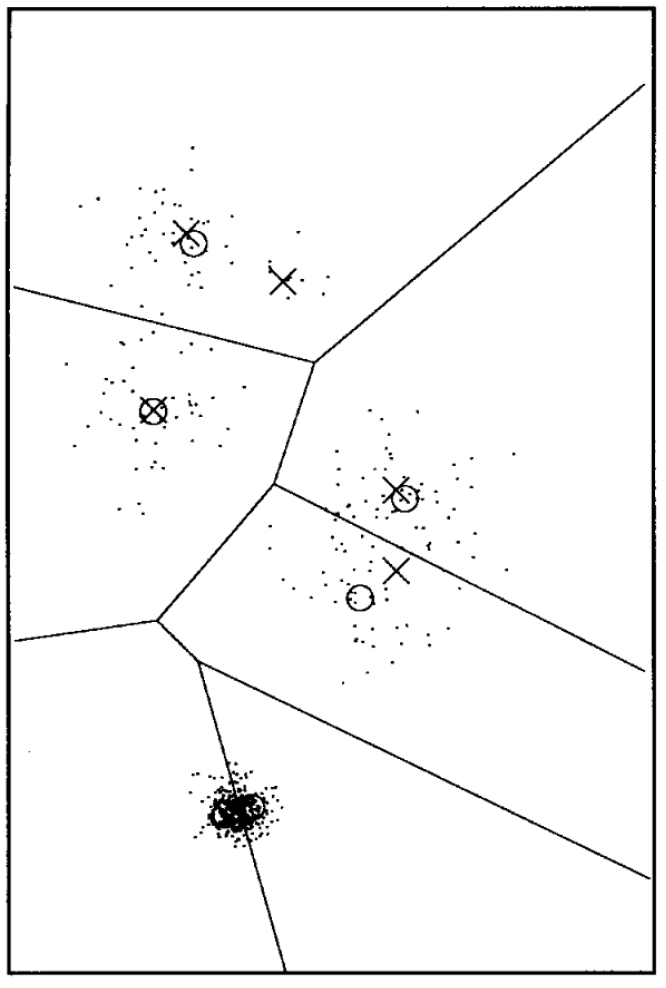
\includegraphics[width=\textwidth]{\dir/k_means_6}
        \caption{$K$-means}
        \label{fig:k_means_6}
    \end{subfigure}
    ~ %add desired spacing between images, e. g. ~, \quad, \qquad, \hfill etc. 
      %(or a blank line to force the subfigure onto a new line)
    \begin{subfigure}[b]{0.4\textwidth}
        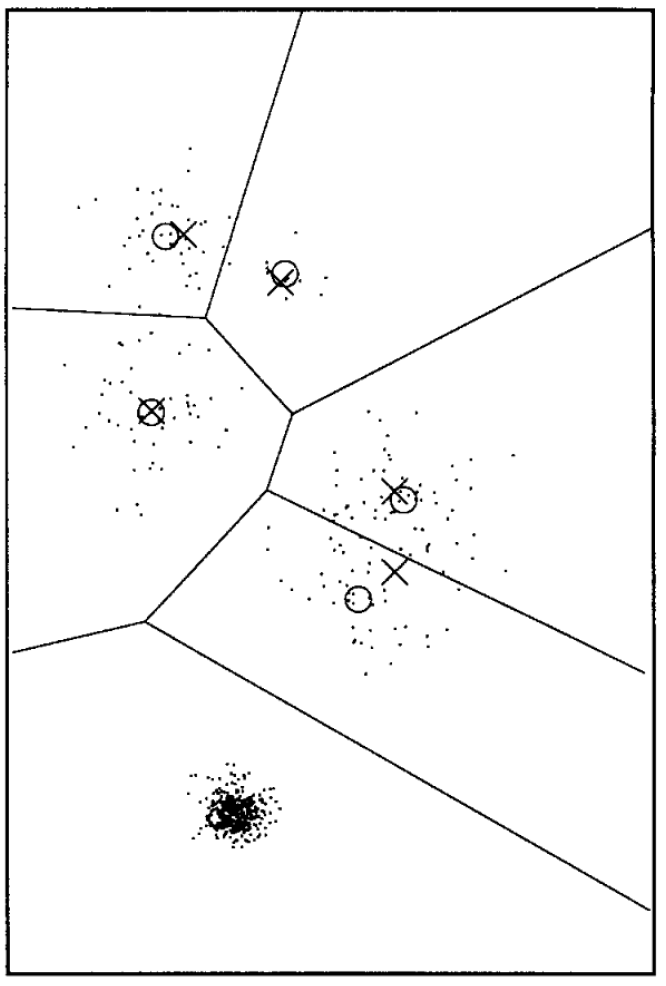
\includegraphics[width=\textwidth]{\dir/da_6}
        \caption{Deterministic annealing}
        \label{fig:da_6}
    \end{subfigure}
    \caption{Comparison of (a) $K$-means and (b) deterministic annealing. The $\times$ marks are the means of the Gaussian components. The $\bigcirc$ marks are the centroids computed by the algorithm.}
    \label{fig:da_vs_kmeans}
\end{figure}

\section{Phase transitions}
\label{sec:phase_transition}

We now study the behavior of the centroids as the temperature decreases.
We will see that, at the beginning when the temperature is high, all centroids
are equal to the sample mean. As a result one can assume that there
is only one cluster. As the temperature decreases, this cluster eventually decomposes into a few clusters, which continue decomposing into more clusters as the temperature keeps decreasing.

Figure~\ref{fig:da_phase_trans}, from Rose~\cite{rose1998deterministic}, illustrates this behavior. The four subfigures show the centroids ($\times$ marks) at four different points of the execution of
deterministic annealing with 9 centroids. Here, $X$ is a sample from a mixture of 9 Gaussians.
The subfigures are sorted by decreasing temperature. The curves in the graphic represent points that have all the same probability of belonging to one particular cluster. Observe how the apparent number of centroids change as the temperature
decreases. In Figure~\ref{fig:da_high_temp}, there seems to be only three centroids,
but what actually happens is that some of the 9 centroids are very close to
each other. Figure~\ref{fig:da_mid1_temp} shows the centroids after the temperature has decreased.
There seems to be now 5 centroids. In Figure~\ref{fig:da_mid2_temp} we have a lower
temperature and now 7 apparent centroids. Finally, in Figure~\ref{fig:da_low_temp}, all 9
centroids are at different locations and close to the means of the Gaussian
mixture.
We now investigate this behavior analytically. We do this through a
sequence of lemmas whose proofs are left as exercises.

\begin{figure}
    \centering
    \begin{subfigure}[b]{0.4\textwidth}
        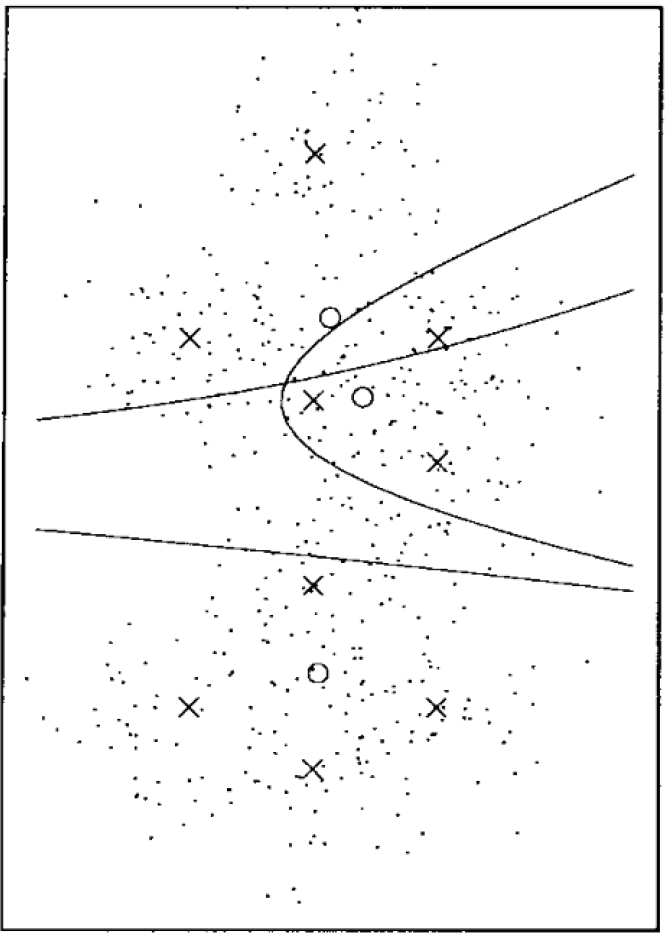
\includegraphics[width=\textwidth]{\dir/da_high_temp}
        \caption{}
        \label{fig:da_high_temp}
    \end{subfigure}
    ~ %add desired spacing between images, e. g. ~, \quad, \qquad, \hfill etc. 
      %(or a blank line to force the subfigure onto a new line)
    \begin{subfigure}[b]{0.4\textwidth}
        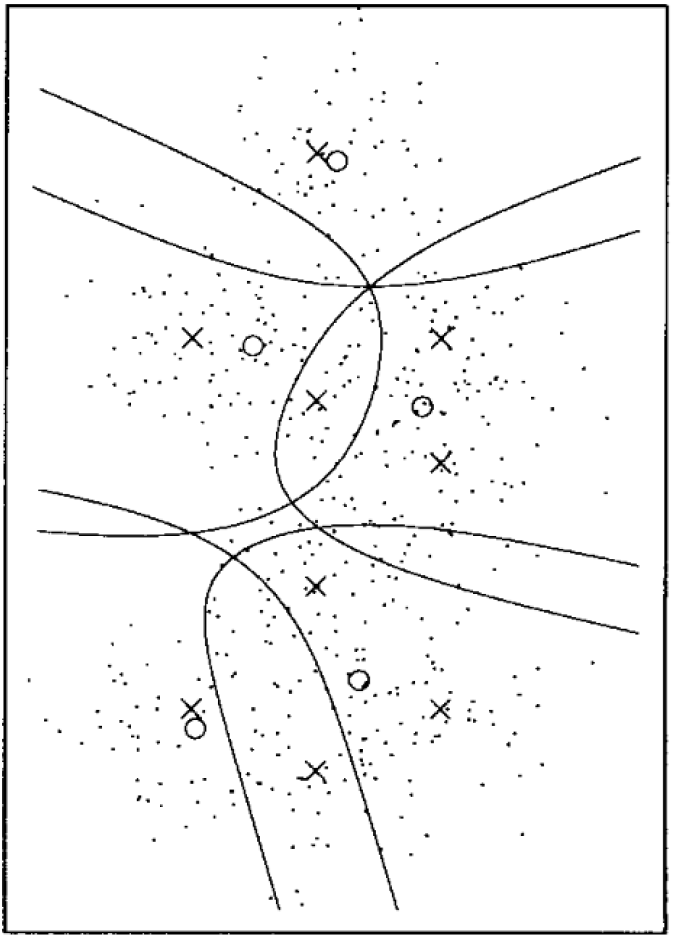
\includegraphics[width=\textwidth]{\dir/da_mid1_temp}
        \caption{}
        \label{fig:da_mid1_temp}
    \end{subfigure}
    
    \begin{subfigure}[b]{0.4\textwidth}
        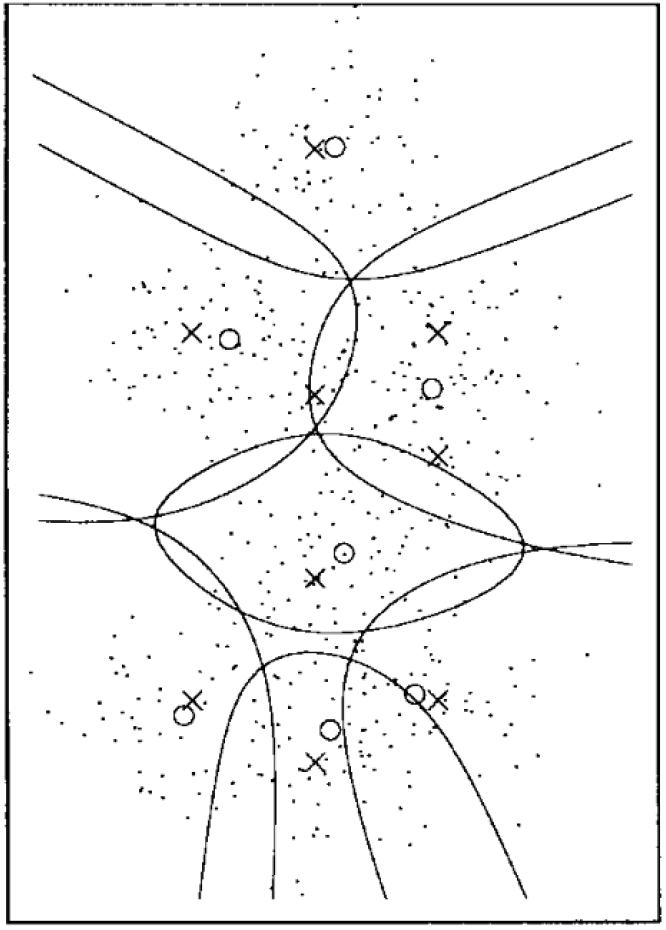
\includegraphics[width=\textwidth]{\dir/da_mid2_temp}
        \caption{}
        \label{fig:da_mid2_temp}
    \end{subfigure}
    ~ %add desired spacing between images, e. g. ~, \quad, \qquad, \hfill etc. 
      %(or a blank line to force the subfigure onto a new line)
    \begin{subfigure}[b]{0.4\textwidth}
        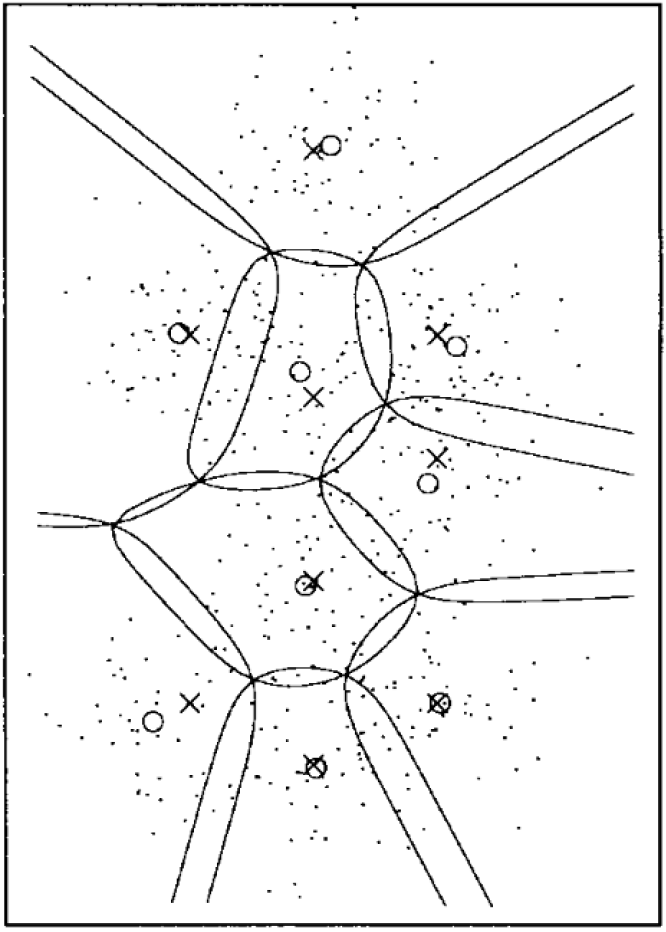
\includegraphics[width=\textwidth]{\dir/da_low_temp}
        \caption{}
        \label{fig:da_low_temp}
    \end{subfigure}
    \caption{}\label{fig:da_phase_trans}
\end{figure}

\subsection{There is only one cluster at a high temperature}

\begin{lemma}
\begin{equation}
\lim_{T \to \infty} \prob\left(C(i) = k \mid \theta, X\right) = \frac{1}{K}.
\end{equation}

\begin{equation}
\lim_{T \to 0} \prob\left(C(i) = k \mid \theta, X\right) = \begin{cases}
1 & \text{ if $\theta_k$ is the centroid closest to $x_k$ and}\\
0 & \text{ otherwise}.
\end{cases}
\end{equation}
\label{lem:da_extreme_temps}
\end{lemma}

\begin{proof}
This is a consequence of Exercise~\ref{ex:gibbs_dist_extreme_temps}.
\end{proof}

\begin{lemma}
For $R(\cdot, \theta, X)$, the $K$-means cost function, maximizing $H[p(\cdot \mid \theta, X)]$ with respect to $\theta$ is equivalent to minimizing
%
\begin{equation}
\mathcal{F}(\theta, X) := -T \sum_{i \leq N}\log \left(\sum_{k \leq K}\exp\left(-\frac{1}{T}\left\|x_i - \theta_{c(i)}\right\|^2\right)\right).
\label{eq:gibbs_free_energy_da}
\end{equation}
%
\label{lem:max_ent_is_min_free_energy_da}
\end{lemma}

\begin{proof}
The proof is similar to that of Lemma~\ref{lem:stationarity_condition} and involves Theorem~\ref{thm:gibbs_factorizes}.
\end{proof}

$\mathcal{F}\left(\theta, X\right)$ is called \emph{the Gibbs free energy (induced by $R(\cdot, \theta, X)$)}.

\begin{theorem}
At $T = 2\lambda$, there is a transition from one to several clusters, where $\lambda$ is the maximum eigenvalue of the sample covariance matrix of $X$. This is the matrix $\frac{1}{n}XX^\top$, where $X$ is seen as a matrix whose columns are all points in the observation.
\label{thm:critical_temp_da}
\end{theorem}

The rest of this section is devoted to prove lemmas that will help prove
this theorem.

Without loss of generality, we assume that $\theta^\infty = 0$. Observe that
when T is sufficiently high, the Hessian $H$ of $\mathcal{F}$ evaluated at $\theta^\infty$ is positive
definite. So new clusters arise when $H$ is no longer positive definite. Our plan is to demonstrate that $H$ stops being positive definite when $T = \frac{1}{2\lambda}$.

The Hessian $H$ can be seen as a block matrix where each block is the
Hessian matrix:
%
\begin{equation}
\frac{\partial F}{\partial \theta_\ell \partial \theta_k}\Bigr|_{\theta^\infty} = 
\left(
\begin{array}{ccc}
\displaystyle
\frac{\partial F}{\partial \theta_{\ell 1} \partial \theta_{k 1}}\Bigr|_{\theta^\infty} & \ldots & \displaystyle\frac{\partial F}{\partial \theta_{\ell 1} \partial \theta_{k d}}\Bigr|_{\theta^\infty}\\
\vdots & \ddots & \vdots\\
\displaystyle\frac{\partial F}{\partial \theta_{\ell d} \partial \theta_{k 1}}\Bigr|_{\theta^\infty} & \ldots & \displaystyle\frac{\partial F}{\partial \theta_{\ell d} \partial \theta_{k d}}\Bigr|_{\theta^\infty}
\end{array}
\right).
\end{equation}
%
From now on, we restrict the domain of $\frac{\partial F}{\partial \theta_\ell \partial \theta_k}$ to a ball $\mathcal{B}$ centered at the origin with a sufficiently small radius so that $\theta_k^\top \theta_\ell$ is insignificant, for every $k, \ell \leq K$. In particular, $\theta_{km}\theta_{\ell m'}$ is insignificant, for every $k, \ell \leq K$ and every $m, m' \leq d$.

\begin{lemma}
Inside $\mathcal{B}$,
%
\begin{equation}
\frac{\partial F}{\partial \theta_k} \approx -\frac{2}{T}\sum_{i \leq N} \frac{A_{ik}}{B_i},
\end{equation}
%
where
%
\begin{equation}
A_{ik} = (x_i - \theta_k)\left(1 + \frac{2}{T}x_i^\top \theta_i\right) \qquad \text{and} \qquad B_i = \sum_{k' \leq K}\left(1 + \frac{2}{T}x_i^\top \theta_{k'}\right).
\end{equation}
%
\label{lem:approx_deriv}
\end{lemma}

\begin{proof}
Start from
%
\begin{equation}
\frac{\partial F}{\partial \theta_k} = - \frac{2}{T} \sum_{i \leq N} \prob\left(C(i) = k \mid \theta, X\right)(x_i - \theta_k).
\label{eq:start_eq_da}
\end{equation}
%
Observe that, inside $\mathcal{B}$,
%
\begin{equation}
\left\|x_i - \theta_k\right\|^2 = \left\|x_i\right\|^2 - 2x_i^\top\theta_k + \left\|\theta_k\right\|^2 \approx \left\|x_i\right\|^2 - 2x_i^\top \theta_k.
\end{equation}
%
Hence,
%
\begin{align}
\exp\left(- \frac{1}{T}\left\|x_i - \theta_k\right\|^2\right) &\approx \exp\left(-\frac{1}{T}\left\|x_i\right\|^2\right)\exp\left(\frac{2}{T}x_i^\top \theta_k\right)\\
&\approx \exp\left(-\frac{1}{T}\left\|x_i\right\|^2\right)\left(1 + \frac{2}{T}x_i^\top \theta_k\right).\\
\end{align}
%
Therefore,
%
\begin{align}
\prob\left(C(i) = k \mid \theta, X\right) &= \frac{\exp\left(-\frac{1}{T}\left\|x_i - \theta_k\right\|^2\right)}{\sum_{k' \leq K}\exp\left(-\frac{1}{T}\left\|x_i - \theta_{k'}\right\|^2\right)}\\
&\approx \frac{\exp\left(-\frac{1}{T}\left\|x_i\right\|^2\right)\left(1 + \frac{2}{T}x_i^\top \theta_k\right)}{\sum_{k' \leq K}\exp\left(-\frac{1}{T}\left\|x_i\right\|^2\right)\left(1 + \frac{2}{T}x_i^\top \theta_{k'}\right)}\\
&= \frac{\left(1 + \frac{2}{T}x_i^\top \theta_{k}\right)}{\sum_{k' \leq K}\left(1 + \frac{2}{T}x_i^\top \theta_{k'}\right)}.\label{eq:simplified_factor_prob}
\end{align}
%
The result follows from plugging (\ref{eq:simplified_factor_prob}) in Equation~(\ref{eq:start_eq_da}).
\end{proof}

\begin{lemma}
\begin{equation}
\frac{\partial F}{\partial \theta_\ell \partial \theta_k}\Bigr|_{\theta^\infty} = \underbrace{\frac{2N}{K}\mathbb{I}\left\{\ell = k\right\}\left(I - \frac{2}{TN}XX^\top\right)}_{P} + \underbrace{\frac{2}{K^2}XX^\top.}_Q
\end{equation}
Here, $\mathbb{I}\left\{\ell = k\right\}$ is the identity matrix when $\ell = k$ and the zero matrix otherwise.
\end{lemma}

\begin{proof}
For $m, m' \leq d$, apply the quotient rule to show that
%
\begin{equation}
\frac{\partial F}{\partial \theta_{\ell m'} \partial \theta_{k m}}\Bigr|_{\theta^\infty}
=
-2\sum_{i \leq N}\left(\frac{1}{B_i}\Bigr|\frac{\partial A_{ikm}}{\partial \theta_{\ell m'}}\Bigr|_{\theta^\infty}\right) + 2 \sum_{i \leq N} \frac{A_{ikm}\Bigr|_{\theta^\infty}}{\left(B_i \Bigr|_{\theta^\infty}\right)^2}\left(\frac{\partial B_i}{\partial \theta_{\ell m'}}\Bigr|_{\theta^\infty}\right).
\end{equation}
%
Observe now that
%
\begin{equation}
A_{ik}\Bigr|_{\theta^\infty} = x_i, \quad B_i \Bigr|_{\theta^\infty} = K, \quad \text{and} \quad \frac{\partial B_i}{\partial \theta_\ell}\Bigr|_{\theta^\infty} = x_i.
\end{equation}
%
Therefore,
%
\begin{equation}
\frac{\partial F}{\partial \theta_{\ell} \partial \theta_{k}}\Bigr|_{\theta^\infty}
= - \frac{2}{K}\left(\frac{\partial}{\partial \theta_\ell}\sum_{i \leq N}A_{ik}\right)\Bigr|_{\theta^\infty} + \frac{2}{K^2}\sum_{i \leq N}x_i x_i^\top.
\label{eq:estimate_hessian_da}
\end{equation}
%
Show now that
%
\begin{equation}
\sum_{i \leq N}A_{ik} = \left(\frac{2}{T}XX^\top - NI\right)\theta_k.
\end{equation}
%
This implies that
%
\begin{equation}
\left(\frac{\partial}{\partial \theta_\ell}\sum_{i \leq N}A_{ik}\right)\Bigr|_{\theta^\infty} = N\mathbb{I}\left\{\ell = k\right\}\left(\frac{2}{TN}XX^\top - I\right).
\end{equation}
%
Plugging this into Equation~\ref{eq:estimate_hessian_da} yields the desired result.
\end{proof}

Observe that, with high probability, $Q$ is positive semi-definite.

\begin{lemma}
Let $Q$ be a positive semi-definite matrix. Let $H$ be a block
matrix where the block $(i,j)$ is given by
%
\begin{equation}
H[i,j] = \mathbb{I}\left\{\ell = k\right\} P + Q.
\end{equation}
%
Then $H$ is positive-definite iff $P$ is.
\label{lem:aux_lemma_ross}
\end{lemma}

\begin{proof}
See Rose's doctoral thesis~\cite{rose1991deterministic}.
\end{proof}

We now prove Theorem~\ref{thm:critical_temp_da}. Recall that the temperature at which $\theta^\infty$ stops being the unique minimum is the temperature at which the Hessian matrix $H$ evaluated at $\theta^\infty$ stops begin positive definite. By Lemma~\ref{lem:aux_lemma_ross}, this occurs when 
%
\begin{equation}
P = I - \frac{2}{TN}XX^\top
\end{equation}
%
is no longer positive definite, which occurs when
%
\begin{equation}
0 = \left|I - \frac{2}{TN}XX^\top\right| = \left|\frac{T}{2}I - \frac{1}{N}XX^\top\right|.
\end{equation}
%
That is, when $T/2$ is an eigenvalue of $\frac{1}{N}XX^\top$. Since $R$ starts at a very
large value and is gradually decreased, we conclude that the temperature at
which more clusters appear is at $T = 2\lambda$ where $\lambda$ is the largest eigenvalue of $\frac{1}{N}XX^\top$. This concludes the proof.

\section{Deterministic annealing and posterior agreement}
\label{sec:da_pa}

There is still an open question regarding deterministic annealing. What
is the number of clusters that we should use? More generally, at which
temperature we should stop the execution of deterministic annealing? The
posterior agreement principle recommends to have two observations $X'$ and
$X''$ and compute the temperature that maximizes the posterior agreement
kernel
%
\begin{equation}
\kappa(X', X'') = \sum_c p(c \mid X') p(c \mid X'').
\end{equation}
%
Observe that for the two probabilities to make sense, we must have $X' = \{x'_1, \ldots, x'_M\}$ and $X'' = \{x''_1, \ldots, x''_N\}$ of equal size. We assume from
now on that this is the case. Furthermore, we assume that $x'_i$ and $x''_i$, for $i \leq N$, are
two observations of one same object. The more general scenario is studied
by Buhmann~\cite{buhmann2010information}.

An analytical method to maximize $\kappa(X', X'')$ with respect to the temperature
is unknown. Moreover, the posterior agreement kernel seems to
be computationally intractable, as it is a sum over $K^N$ objects. Fortunately,
the factorization of the Gibbs distribution makes it computationally
tractable.

\begin{exercise}
Show that
%
\begin{equation}
\sum_{c}p(c \mid X') p(c \mid X'') = \prod_{i \leq N}\sum_{k \leq K}\prob\left(C(i) = k \mid X'\right)\prob\left(C(i) = k \mid X''\right).
\end{equation}
%
Show also that computing this takes $O(NK)$-time.
\end{exercise}

Our plan is then to select a set of candidate temperatures and pick the
one with the highest $\kappa(X', X'')$ as the stopping temperature. We can implement
this plan during the execution of deterministic annealing. Observe
that the while loop of of Algorithm~\ref{algo:da_algo_da} gives as a sequence of decreasing
temperatures. Therefore, we can compute $\kappa(X', X'')$ at each iteration
with the current temperature. We can keep track of these kernel values.
The value of $\kappa(X', X'')$ has been observed empirically to be low when the
temperature is high, then it increases as the temperature is lowered, and
eventually it starts decreasing. Hence, we can keep track of how the kernel
values change as deterministic annealing decreases the temperature. After
observing, for a certain amount of iterations, that $\kappa(X', X'')$ is no longer
increasing and starts decreasing, we can stop the annealing and choose as
stopping temperature the one that yielded the largest $\kappa(X', X'')$.

\chapter{Information bottleneck}

To be done in 2022.

\chapter{Constant-shift embedding}

To be done in 2022.

\chapter{Pairwise clustering}

To be done in 2022.

\chapter{Mean-field approximation}

To be done in 2022.

\renewcommand{\dir}{posterior_agreement}
\chapter{An information-theoretic foundation for posterior agreement}
\chaptermark{Posterior agreement}

%\newcommand{\prob}{\mathbb{P}}
%\newtheorem{assumption}{Assumption}
\newtheorem{objective}{Objective}

%
%\newcommand{\carlos}[1]{}
%\newcommand{\fcarlos}[1]{}
%\newcommand{\todo}[1]{}
%
%\theoremstyle{definition}
%
%\newtheorem{definition}{Definition}
%\newtheorem{example}{Example}
%\newtheorem{theorem}{Theorem}

\section{Introduction}

This chapter proposes an information-theoretic foundation for posterior agreeement, as a method for validating clustering algorithms, originally proposed by Joachim Buhmann~\cite{buhmann2010information} and studied by Alex Gronskiy as part of his doctoral thesis~\cite{gronskiy2018statistical}.
 
Posterior agreement can be understood as a method for \emph{validating algorithms} that solve stochastic optimization problems of the form
%
$$\min_{c} \mathbb{E}_X\left[R(c, X)\right].$$
% 
Here, $R(c, X)$ is the result of evaluating a cost function on a candidate solution $c$ on an instance of the problem described by the random variable $X$. The expectation is computed with $X$'s distribution.

In posterior agreement, we assume that an algorithm is a function that computes, from a given observation $X'$, a \emph{posterior distribution} $p(\cdot \mid X')$ over a finite space $\mathcal{C}$ of possible solutions. Every algorithm can be converted into such an algorithm, even if it is deterministic. In this case, the posterior distribution is just a distribution that assigns probability mass one to the algorithm's output.

Posterior agreement assesses the performance of an algorithm by computing the \emph{expected log posterior agreement}:
%
\begin{equation}
\mathbb{E}_{X', X''} \log \left(\left|\mathcal{C}\right|\kappa\left(X', X''\right)\right),
\label{eq:overview_exp_log_post_agr}
\end{equation}
%
where $\kappa\left(X', X''\right)$ is the \emph{posterior agreement kernel}:
%
$$\kappa\left(X', X''\right) := \sum_{c \in \mathcal{C}} p(\cdot \mid X')p(\cdot \mid X'').$$

The expected log posterior agreement requires the joint probability distribution of $X'$ and $X''$, which is often unknown. One only has access to a handful of observations, at least two: $X'$ and $X''$. In this case, one can use the \emph{empirical log posterior agreement}:
%
\begin{equation}
\log \left(\left|\mathcal{C}\right|\kappa\left(X', X''\right)\right).
\label{eq:overview_emp_log_post_agr}
\end{equation}

Moreover, the empirical log posterior agreement is intended to be a metric to compare different algorithms. Therefore, it is often sufficient to measure $\kappa\left(X', X''\right).$

%We show how posterior agreement can compare, for example, Prim's, Kruskal's, and the reverse-delete algorithm for computing spanning trees for graphs whose edge weights are defined by random variables, as in the example above. Posterior agreement can also compare among different cost functions and hyperparameter values, when training machine learning models.

Therefore, posterior agreement advocates that, in the context of stochastic optimization, \emph{algorithms should aim for maximizing the posterior agreement kernel, given two instances of the problem}, rather than minimizing the cost function for either instance or an aggregate of these instances.

The proofs given in this chapter works for algorithms that satisfy the following \emph{asymptotic equipartition property}. As $n \to \infty$, $\log \left(\left|\mathcal{C}\right|\kappa(X', X'')\right)$ converges in probability to
%
\begin{equation}
\mathbb{E}_{X', X''}\left[\log \left(\left|\mathcal{C}\right|\kappa(X', X'')\right)\right].
\end{equation}
%
Such property is satisfied by many of the algorithms studied in this script, like deterministic annealing and histogram clustering. Furthermore, if an algorithm produces distributions that can be sufficiently well approximated by a mean-field approximation, then it is possible to demonstrate that they also fulfil this asymptotic equipartition property.

\begin{exercise}
Show that deterministic annealing (DA) satisfies the asymptotic equipartition property.
\end{exercise}

\begin{proof}
Recall that the distribution $p(\cdot \mid \theta, X')$ computed by DA on a given sample of points $X' = \{x'_1, \ldots, x_n'\}$ factorizes as follows:
%
\begin{equation}
p(c \mid \theta, \theta, X') = \prod_{i \leq n} p(c(i) \mid \theta, x'_i),
\end{equation}
%
where
%
\begin{equation}
p(k \mid \theta, x'_i) \propto \exp\left(-\frac{1}{T}\left\|x_i - \theta_k\right\|^2\right).
\end{equation}
%
From Exercise~\ref{ex:pa_factorizes_da}, we know that
%
\begin{equation}
\kappa\left(X', X''\right) = \prod_{i \leq n} \sum_{k \leq K} p(k \mid \theta, x'_i)p(k \mid \theta, x''_i).
\end{equation}
%
Therefore,
%
\begin{equation}
\log \left(\left|\mathcal{C}\right|\kappa\left(X', X''\right)\right) = \log \left|\mathcal{C}\right| + \sum_{i \leq n}\log \sum_{k \leq K} p(k \mid \theta, x'_i)p(k \mid \theta, x''_i).
\end{equation}
%
Now, if we take the limit as $n \to \infty$ of both sides, and apply the law of large numbers, we have that, as $n \to \infty$, $\log \left(\left|\mathcal{C}\right|\kappa\left(X', X''\right)\right)$ converges in probability to
%
\begin{equation}
\log \left|\mathcal{C}\right| + n \mathbb{E}_{x', x''}\left[\log \sum_{k \leq K} p(k \mid \theta, x')p(k \mid \theta, x'')\right],
\label{eq:result_conv_prob_pa}
\end{equation}
%
Finally, observe that
%
\begin{align}
\mathbb{E}_{X', X''}\left[\log \kappa\left(X', X''\right)\right]
&= \mathbb{E}_{X', X''}\left[\sum_{i \leq n}\log \sum_{k \leq K} p(k \mid \theta, x'_i)p(k \mid \theta, x''_i)\right]\\
&= \sum_{i \leq n}\mathbb{E}_{X', X''}\left[\log \sum_{k \leq K} p(k \mid \theta, x'_i)p(k \mid \theta, x''_i)\right]\\
&= \sum_{i \leq n}\mathbb{E}_{x'_i, x''_i}\left[\log \sum_{k \leq K} p(k \mid \theta, x'_i)p(k \mid \theta, x''_i)\right]\\
&= n\mathbb{E}_{x', x''}\left[\log \sum_{k \leq K} p(k \mid \theta, x')p(k \mid \theta, x'')\right].\\
\end{align}
%
Substituting this in Equation~\ref{eq:result_conv_prob_pa} yields the desired result.
\end{proof}

\begin{corollary}
Consider an algorithm that, when given as input a sample $X'$, outputs a distribution $p(\cdot \mid X')$. Assume that this distribution admits a mean-field approximation such that
%
\begin{equation}
p(c \mid X') \approx \prod_{i \leq n} q(c_i \mid x_i').
\end{equation}
%
Then this algorithm fulfils the asymptotic equipartition property.
\end{corollary}

The proof is analogous to the one above.

\todo{Organization of these notes.}

\section{Motivation}

\begin{figure}
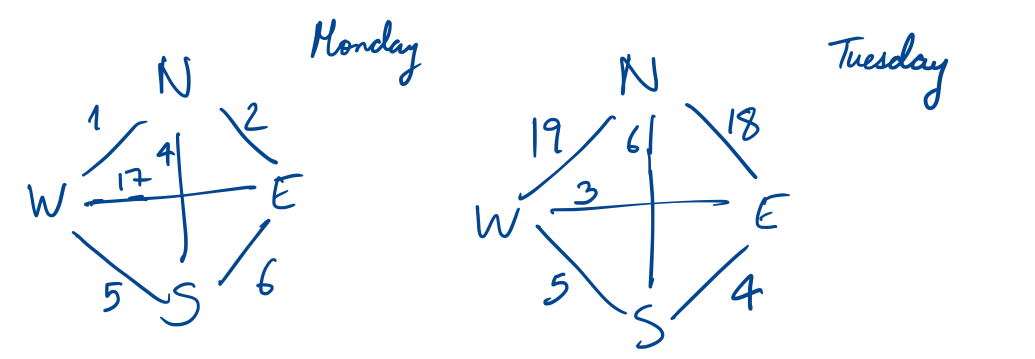
\includegraphics[width=\textwidth]{\dir/mst_setup.png}
\caption{A graph with its observed edge weights for two different days.}
\label{fig:mst_setup}
\end{figure}

Figure~\ref{fig:mst_setup} gives two graphs modeling a city with four main locations: North, East, South, and West. There is a road connecting any two different locations and, depending on the day, traversing that road by car takes some amount of time. The number labeling each edge indicates that time. Observe that the time varies with each day.

Consider the minimum spanning tree of each of these two graphs. For Monday's graph, the tree is the one with North at the root and all other locations as children of North. For Tuesday's graph, the tree is the one with South at the root and all other locations as children of South. We call these two trees the North and South trees, respectively.

Can we estimate from this information what Wednesday's graph's minimum spanning tree will look like?

The city graph can be understood as a random variable $X$. More precisely, it is a collection of 6 random variables, each of them defining an edge's weight on a particular day. Hence, the weight $R(c, X)$ of a tree $c$ in $X$, which is the sum of the edge weights in $c$, is also a random variable. We can then formulate the problem of the minimum spanning tree for our case as the following stochastic optimization problem:
%
\begin{equation}
\arg \min_{c \in \mathcal{C}} \mathbb{E}_X\left[R(c, X)\right],
\label{eq:stoch_min_span_tree}
\end{equation}
%
where $\mathcal{C}$ denotes all spanning trees of the city graph.

This type of optimization problems appear very often in combinatorial optimization and statistical learning. One challenge in this type of optimization problems is that we do not know $X$'s probability distribution.
One natural way to go around this issue and approximately solve Problem~\ref{eq:stoch_min_span_tree} is to substitute $\mathbb{E}\left[R(c, X)\right]$ with an \emph{empirical estimate}:
%
$$\mathbb{E}\left[R(c, X)\right] \approx \frac{1}{N}\sum_{i \leq N} R(c, X_i),$$
%
where $\left\{X_1, \ldots, X_n\right\}$ is a sample of observed values of $X$.

When $n$ is sufficiently large and each $X_i$ is independent from the others, then by the law of large numbers, this becomes a good approximation of $\mathbb{E}\left[R(c, X)\right]$. We call the \emph{empirical risk minimizer} the solution of the problem:
%
\begin{equation}
\arg \min_{c \in \mathcal{C}} \sum_{i \leq n}\left[R(c, X_i)\right],
\label{eq:erm}
\end{equation}

Unfortunately, the empirical risk minimizer does not always minimize the expected risk, especially, when the sample size $n$ is small, as we saw in the random array problem in Section~\ref{sec:random_array}. The empirical risk minimizer can overfit the sample and, therefore, fail to generalize to other samples.

One can prevent such overfitting with techniques like regularization. This makes the solutions less sensitive to the noise in the sample. However, such techniques may lead to solutions that are too insensitive to the signal in the sample, failing to minimize the expected cost as well.

Solving Problem~\ref{eq:stoch_min_span_tree} requires designing algorithms that strike a balance between two extremes. On one hand, algorithms may \emph{overfit} and produce solutions that are too sensitive to the noise in the sample. On the other hand, algorithms may \emph{underfit} and produce solutions that are too insensitive to the signal in the sample. These two extremes are illustrated in Figure\ref{fig:clustering}\todo{} for the problem of clustering. In the overfitting extreme, an algorithm may just make each point in the sample its own cluster (and this solution would actually minimize the expected cost). In the undefitting extreme, an algorithm may just put all points in the sample into one single cluster. The overfitting algorithm minimizes the cost, but is extremely sensitive to noise in the data, whereas the underfitting algorithm is very robust, but fails to minimize the expected cost. Can we find a common ground between these two?

%We present later scenarios where the empirical risk minimizer is not the best solution we can obtain, especially when we have only very few observations. One example, presented in Section~\ref{sec:random_array} is the problem of computing the minimum of an array $X = \left(X_1, \ldots, X_n\right)$ of random variables. Given just two observations $X^1$ and $X^2$, estimating $\min_i \mathbb{E}_X[X_i]$ with the empirical risk minimizer is not the best we can do. We also showed in that section, how combining maximum entropy and posterior agreement yielded a better estimator.

\subsection*{Posterior agreement}

To find a solution to this apparent dilemma, posterior agreement has been proposed. This is a metric to evaluate how well an algorithm proposes solutions that minimize the expected cost and, at the same time, that are robust to the noise in the data.

Why is posterior agreement a good metric for validating algorithms? Why should we use it instead of other more standard criteria like cross-validation or the minimum description length? These notes argue that posterior agreement is effective, \emph{because it quantifies the amount of information that algorithms extract from phenomena}.
%Moreover, there are also scenarios where it is not possible to get a sufficiently large sample of observed values to estimate $X$'s distribution. \carlos{Give examples of such scenarios}

\section{Overview}
%
%For example, in the context of computing the city graph's minimum spanning tree, the phenomenon is the probability distribution that governs the edge weights that we observe on a particular day. An observation $X'$ defines the actual edge weights of a particular day. The signal we want to retrieve is a distribution $p(\cdot)$ over the spanning trees. For a spanning tree $c$, $p(c)$ measures how much we believe that minimizes $\mathbb{E}\left[R(c, X)\right]$.

Posterior agreement originates from formalizing an algorithm $\mathcal{A}$ \emph{as a communication channel} by which a sender and a receiver communicate outputs from $\mathcal{A}$. The main argument justifying posterior agreement states the following. The amount of information conveyed by an algorithm can be measured by the \emph{capacity} of that communication channel, where the capacity, as we explain later, defines the maximum number of distinguishable messages that can be communicated through the channel.

This section gives an informal overview of this main argument. The later sections formalize this argument. We start with a recap of Shannon's channel coding theory and then show how to apply it to represent and analyze algorithms as communication channels.

\subsubsection*{Shannon's channel coding theorem}

Consider a channel by which a sender can transmit bits to a receiver. Assume that the channel is noisy in the sense that a bit can be flipped during transmission with probability $\epsilon < 0.5$. The sender and the receiver agree on transmitting only bitstrings of length $n$. We call these bitstrings \emph{codewords}. 

Observe that if $\epsilon = 0$, then the sender can reliably communicate $2^n$ different messages to the receiver, by agreeing in advance with the receiver on a way to encode each message as one codeword of length $n$. This correspondence is called a \emph{code} and will be formally defined in Section~\ref{sec:shannon_theorem}.

In practice, $\epsilon > 0$. Therefore, the sender and the receiver need to agree on a code that is robust to the channel's noise. We now show two examples of codes:

\begin{itemize}
\item They could agree on just 2 messages, encoded as $00\ldots0$ and $11\ldots 1$, respectively. If the codeword length is sufficiently large, then with high probability, less than half of the bits will be flipped during transmission. As a result, the receiver can almost surely identify the message from the received codeword, by just counting the frequency of each bit in the codeword.
\item They agree on sending $2^n$ messages, each encoded with a unique codeword of length $n$. With high probability, some of the bits will be flipped during transmission and the receiver will fail to identify the message that the sender tried to communicate.
\end{itemize}

Observe that these two codes represent two extremes, as $n \to \infty$. On one hand, the first code is robust: it communicates only 2 messages, but with high probability of success. On the other hand, the second code communicates the maximum number of possible messages, but with low probability of success, as it is very sensitive to the channel's noise. One can also imagine other codes that strike a balance between the number of messages to be communicated and the success probability. Observe how these two extremes correspond to the two extremes of overfitting and underfitting. 

Shannon's coding theorem answers the following question. \emph{What is the code that maximizes the number of messages that the sender can communicate to the receiver, while attaining a probability of success close to 1, as $n \to \infty$?} When $\epsilon > 0$, this number is clearly below $2^n$, but since $\epsilon < 0.5$, this number must be positive. Shannon shows that this number is $2^{nc}$, where $c$ is \emph{the channel's capacity}, a quantity that is defined by the channel. Therefore, channels with higher capacity allow the communication of more messages at the same codeword length.

\subsubsection*{Posterior agreement}

Posterior agreement originates by adapting Shannon's coding theorem to the context of algorithms. This requires a way of modeling an algorithm $\mathcal{A}$ as a communication channel $C_{\mathcal{A}}$, where a sender communicates outputs from $\mathcal{A}$ to a receiver. We do this in these notes and argue that the capacity of $C_{\mathcal{A}}$ is defined by $\mathcal{A}$'s ability to compute robust solutions that minimize the expected cost. That is, if $\mathcal{A}$ is a robust minimizer of the expected cost, then it is possible to communicate many more messages through $C_{\mathcal{A}}$ than when $\mathcal{A}$ is sensitive to noise or when $\mathcal{A}$ is a poor minimizer of the expected cost.

We give an informal overview of this argument next. A rigorous argument is given in Section~\ref{sec:comm_protocol}.

We assume given an \emph{instance space} $\mathcal{X}$, comprising all possible observations, and a \emph{solution space} $\mathcal{C}$, comprising all possible solutions. A phenomenon is then a probability distribution over $\mathcal{X}$. We assume that algorithms intending to solve Problem~\ref{eq:stoch_min_span_tree} receive in the input an observation $X'$ and output a distribution $p(\cdot \mid X')$ over $\mathcal{C}$.

For our analysis, we assume that each instance space contains all observations of a given ``size'' $n \in \mathbb{N}$. This size $n$ is a notion that measures the observations' and phenomena's complexity. For example, in the minimum spanning tree problem, an instance space contains only all weighted graphs with a fixed number $n$ of vertices.

For an algorithm $\mathcal{A}$, we define a communication channel $C_{\mathcal{A}}$ that works as follows. To use the channel, a sender picks an instance $X'$, drawn from a phenomenon $p_X$, computes and inputs $p(\cdot \mid X')$ to the channel. The channel replaces $p(\cdot \mid X')$ with $p(\cdot \mid X'')$, where $X''$ is a fresh new instance drawn from $p_X$. The channel outputs $p(\cdot \mid X'')$ to the receiver.

We now emphasize the key insight of this modeling. If $\mathcal{A}$ is robust to the fluctuations in $X'$, then there should not be much difference between $p(\cdot \mid X')$ and $p(\cdot \mid X'')$. In contrast, if $\mathcal{A}$ is very sensitive to the fluctuations in $X'$, then $p(\cdot \mid X')$ and $p(\cdot \mid X'')$ may be very different. Hence, $\mathcal{A}$'s robustness to noise defines how many different ``messages'' can we send through this channel. We conclude then that $\mathcal{A}$'s robustness is measured by the capacity of this channel $C_{\mathcal{A}}$. This capacity, as we show in Section~\ref{sec:comm_protocol}, can be estimated by the expected log posterior agreement. For this reason, we argue that algorithms intended to solve Problem~\ref{eq:stoch_min_span_tree} shall be measured by their expected log posterior agreement.

%Observe the following analogies to Shannon's coding theory. Channels have a capacity that define the maximum number of distinguishable messages that can be communicated. Channels with higher capacity are preferable, as they allow more different messages to be communicated. Analogously, we argue that algorithms can be modeled as channels and, therefore, have a capacity, which we later show to be the expected log posterior agreement. Hence, we argue that algorithms with higher expected log posterior agreement are preferable, as they allow more different messages to be communicated.

\subsubsection*{Protocol overview}

We now introduce a protocol describing a code by which a sender can communicate messages to a receiver. Let $\mathcal{A}$ be an algorithm intending to solve Problem~\ref{eq:stoch_min_span_tree}. In our case, a message is a phenomenon and a codeword is the output $p(\cdot \mid X')$ of $\mathcal{A}$ when given an observation $X'$ from a phenomenon as input. 
%Analogous to Shannon's coding theorem, the sender and the receiver aim to maximize the number of different messages that the sender can communicate, while ensuring that the receiver's probability of success goes to 1 as $n \to \infty$.

Figure~\ref{fig:overview_protocol} illustrates the idea behind the protocol. The sender must describe a phenomenon $q$ to a receiver through a noisy channel. The sender makes an observation $X'$ from $q$, uses $\mathcal{A}$ to compute $p(\cdot \mid X')$, and sends through the channel to the receiver. The channel is noisy and we represent its noise by replacing $p(\cdot \mid X')$ with $p(\cdot \mid X'')$, where $X''$ is another observation from $q$. The receiver succeeds if he is able, using $p(\cdot \mid X'')$, to identify $q$. Observe how this protocol measures the informativeness of an algorithm by the ability of the receiver to identify phenomena, given the algorithm's output.

\begin{figure}
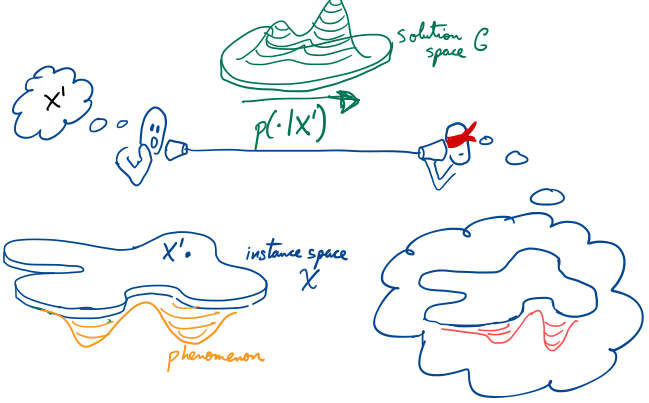
\includegraphics[width=\textwidth]{\dir/overview_protocol.png}
\caption{}
\label{fig:overview_protocol}
\end{figure}

We remark that this protocol is just a thought experiment. The protocol is computationally impossible for many interesting optimization problems. This is because the protocol requires that we know the underlying distribution behind the observations of one phenomenon. This is not possible in most of the cases. Nonetheless, the protocol provides a formal justification and motivation for posterior agreement.

\subsubsection*{Protocol example}

We now give a more precise overview by showing how posterior agreement works with a simple example. Let $\mathcal{A}_1$ and $\mathcal{A}_2$ be two algorithms that estimate the mean of a univariate distribution, given only a sample from that distribution. For example, $\mathcal{A}_1$ fits a Gaussian to the sample via maximum-likelihood estimation whereas $\mathcal{A}_2$ does the same, but only using only the maximum and the minimum of that sample. Suppose that both algorithms output Gaussian distributions that indicate where they believe that the mean is. 

The protocol works as follows. Fix $n \in \mathbb{N}$, which denote the size of all the observations in the instance space. In our case, $n$ denotes the sample size. The sender and the receiver are given the algorithm under evaluation $\mathcal{A}_i$ and then they choose the size $m_n \in \mathbb{N}$ of the set of messages that they the sender will attempt to communicate. Recall that they want to choose $m_n$ as large as possible. However, a large $m_n$ increases the probability $P_n$ that the receiver fails to recognize the message from the codeword transmitted by the sender. We later see that the best choice for $m_n$ is defined by $\mathcal{A}_i$. 

The protocol proceeds then as follows:

\begin{enumerate}
\item\label{step:sample_observations} (Figure~\ref{fig:agree_on_code}) The sender and the receiver agree on a set of $m := m_n$ phenomena, which we represent with the probability distributions $q_1, q_2, \ldots, q_m$.
\item (Figure~\ref{fig:agree_on_code}) The sender and the receiver together make one observation $X'_i$ of each phenomenon $q_i$, with $i \leq m$. In this case, an observation is a sample of points from $q_i$. Afterwards, they use $\mathcal{A}_j$, with $j \in \{1, 2\}$, to compute a distribution $p(\cdot \mid X')$ for each observation $X'$.
\item\label{step:choose} (Figure~\ref{fig:noisy_channel}) An observation $X'$ is chosen out of these $m$ observations uniformly at random. $X'$ is given to the sender, but kept secret from the receiver.
\item (Figure~\ref{fig:substitution_maneuver}) The sender sends $p(\cdot \mid X')$ to the receiver through the communication channel $C_{\mathcal{A}_j}$, defined by $\mathcal{A}_j$. This channel replaces $p(\cdot \mid X')$ with $p(\cdot \mid X'')$, where $X''$ is a fresh new observation from the same phenomenon where $X'$ comes from.
\item (Figure~\ref{fig:guessing}) The receiver gets $p(\cdot \mid X'')$ and must now guess which observation in $\{X'_1, \ldots, X'_m\}$ the sender chose in Step~\ref{step:choose}. For this, the receiver uses the natural approach of guessing the observation $\hat{X}$ for which $p(\cdot \mid \hat{X})$ overlaps the most with $p(\cdot \mid X'')$. In other words, the receiver guesses the observation $\hat{X}$ that fulfills:
%
$$\kappa\left(\hat{X}, X'\right) \geq \kappa\left(Y, X'\right), \text{ for all Y.}$$
%
\item If $\hat{X} = X'$, the receiver has succeeded.
\end{enumerate}

\begin{figure}
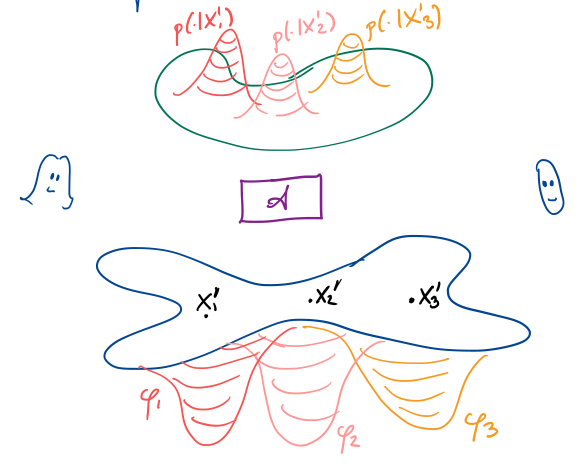
\includegraphics[width=\textwidth]{\dir/agree_on_code.png}
\caption{}
\label{fig:agree_on_code}
\end{figure}

\begin{figure}
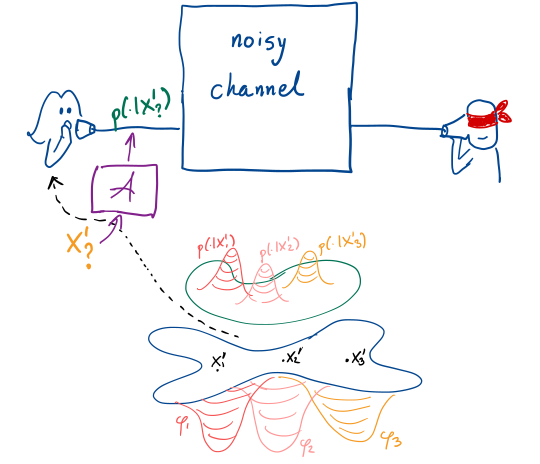
\includegraphics[width=\textwidth]{\dir/noisy_channel.png}
\caption{}
\label{fig:noisy_channel}
\end{figure}

\begin{figure}
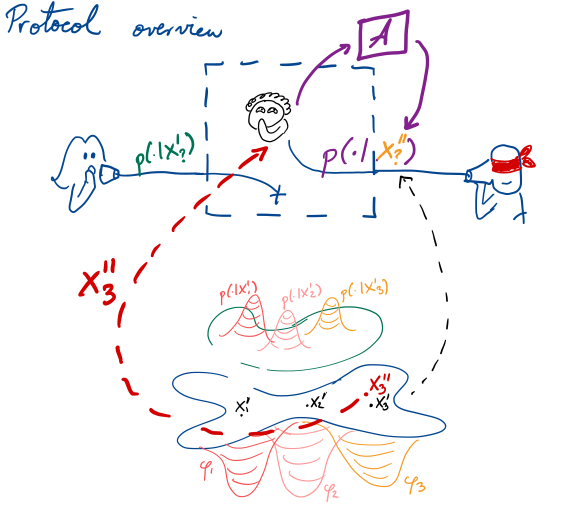
\includegraphics[width=\textwidth]{\dir/substitution_maneuver.png}
\caption{}
\label{fig:substitution_maneuver}
\end{figure}

\begin{figure}
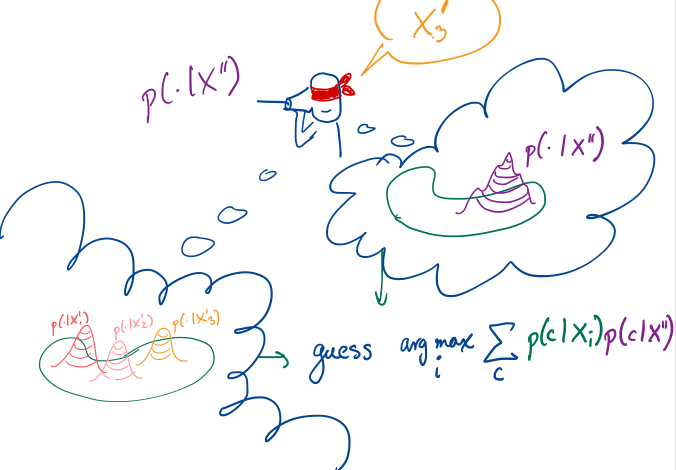
\includegraphics[width=\textwidth]
{\dir/guessing.png}
\caption{}
\label{fig:guessing}
\end{figure}

\subsubsection*{Receiver's probability of failure}

We show in Section~\ref{sub:prob_comm_error} that the receiver's failure probability is bounded above by 
%
$$\exp\left(- \mathbb{E}_{X', X''} \left[\log \left(\left|\mathcal{C}\right|\kappa\left(X', X''\right)\right)\right] + \epsilon \log \left|\mathcal{C}\right| + \log m\right),$$ 
%
where $\epsilon > 0$ is arbitrary, $\mathcal{C}$ is the solution space, and $m$ is the number of observations defined in Step~\ref{step:sample_observations}.

Assume now that $\log \left|\mathcal{C}\right| = \Omega(n)$. This is a reasonable assumption, as for many interesting problems, $\mathcal{C}$ grows exponentially in $n$. Observe that the algorithm can only influence $\kappa\left(X', X''\right)$. If $\epsilon$ is sufficiently small and the algorithm ensures that 
%
$$\mathbb{E}_{X', X''} \log\left(\left|\mathcal{C}\right| \kappa\left(X', X''\right)\right) - \log m = \Omega(n),$$ 
%
then the receiver's failure probability becomes $0$ as $n \to \infty$. The algorithm can ensure this by \emph{maximizing the expected log posterior agreement}. The larger this quantity is, the higher $m$ can be and the more messages the sender can communicate to the receiver.
%
%\begin{figure}
%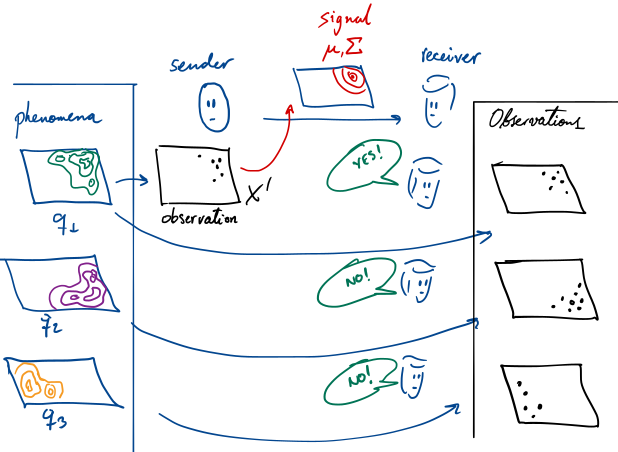
\includegraphics[width=\textwidth]{stoch_opti_as_comm.png}
%\caption{Stochastic optimization as a communication. The sender makes an observation $X'$ of a phenomenon $q_1$. The sender computes a signal $p(\cdot \mid X')$ from that observation and sends it to the receiver.
%The communication is successful if the receiver is able to use the signal to distinguish between future observations from $q_1$ and observations from other different phenomena.}
%\label{fig:mst_setup}
%\end{figure}

\section{Shannon's channel coding theorem}
\label{sec:shannon_theorem}

To properly formulate and analyze the communication protocol above, we build upon Shannon's channel coding theorem. This theorem measures how much information we can optimally send through a communication channel. This section is mainly based on Chapter 7 from Thomas and Cover~\cite{infotheory}.

\subsection{Channels}

We understand a channel as a medium by which one sender can send symbols from a fixed set $\mathfrak{A}$ to a receiver. We allow channels to be noisy, meaning that the symbol $a$ can be altered to another symbol $b$ with probability $p(b \mid a)$ during the transmission through the channel. We do not allow the receiver to give feedback to the sender.

\begin{definition} A \emph{(noisy) channel} is a pair $\left(\mathfrak{A}, \left\{p(\cdot \mid a)\right\}_{a \in \mathfrak{A}}\right)$, where $\mathfrak{A}$ is a set and $p(\cdot \mid a)$, for $a \in \mathfrak{A}$, is a conditional distribution on $\mathfrak{A}$.
\label{def:channel}
\end{definition}

For convenience, we sometimes write just $\mathcal{P}$ to denote the family of distributions $\left\{p(\cdot \mid a)\right\}_{a \in \mathfrak{A}}$. Observe that we assume that transmissions are independent from each other. What the receiver gets does not influence what the user sends or the channel's conditional probabilities in the future.
%
%$\mathfrak{A}$ denotes the set of symbols that can be communicated through the channel. The set $\left\{p(\cdot \mid a)\right\}_{a \in \mathfrak{A}}$ represents the influence of noise in the channel. For $a, b \in \mathfrak{A}$, $p(b \mid a)$ measures the likelihood that the receiver gets $b$ when the sender sends $a$ through the channel.

\begin{example}
The \emph{binary channel} is the channel with $\mathfrak{A} = \{0, 1\}$ and $p(b \mid a) = \mathbb{I}\{a=b\}$, for $a, b \in \mathfrak{A}$, where $\mathbb{I}$ is the indicator function. This is a channel where there is no noise interference.
\end{example}

\begin{example}
The \emph{noisy binary channel} is the binary channel, but with 
%
$$p(b \mid a) 
\begin{cases}
1 - \epsilon & \text{if $a = b$ and}\\
\epsilon & \text{if $a \neq b$.}
\end{cases}
$$
%
Unless stated otherwise, we assume that $0 < \epsilon \leq 0.5$.
\end{example}

\begin{example}
The \emph{typewriter channel} is the channel with $\mathfrak{A} = \{\texttt{a}, \texttt{b}, \ldots, \texttt{z}\}$ and $p(b \mid a) = \mathbb{I}\{a=b\}$, for $a, b \in \mathfrak{A}$, where $\mathbb{I}$ is the indicator function.
\end{example}

\begin{example}
The \emph{noisy typewriter channel} is the channel with $\mathfrak{A} = \{\texttt{a}, \texttt{b}, \ldots, \texttt{z}\}$, but with
%
$$p(b \mid a) 
\begin{cases}
1 - \epsilon & \text{if $a = b$,}\\
\epsilon & \text{if $a = b + 1 \text{ mod } 26$.}
\end{cases}
$$
%
\end{example}

\subsection{Channel capacity}

Which of the channels above sends \emph{the most information per transmission}? Intuitively, a letter has more information than a bit and the presence of noise affects the amount of information we send in one transmission. Indeed, sending one letter through the typewriter channel provides more information than sending one letter through a noisy typewriter channel. Also, a letter has more information than a bit. Hence, we say that the typewriter channel has \emph{the most capacity}: one transmission through this channel carries in average more information than one transmission through any of the other three channels. Similarly, we say that the noisy binary channel has \emph{the least capacity}.

We now formally define channel capacity.

\begin{definition}
For a channel $\left(\mathfrak{A}, \left\{p(\cdot \mid a)\right\}_{a \in \mathfrak{A}}\right)$, its capacity is
%
$$\max_{p(\cdot)} I(S; \hat{S}),$$
%
where $S$ and $\hat{S}$ are random variables denoting a symbol input to the channel and the output symbol, respectively, when $S$ is distributed according to $p(\cdot)$. We refer to $I(S; \hat{S})$ as the channel's \emph{input-output mutual information} and the joint distribution of $S$ and $\hat{S}$ as the \emph{input-output distribution}.
\end{definition}

\begin{example}
For the binary channel, we can reliably send one bit per transmission. This corresponds to the channel's capacity,
%
$$\max_{p(\cdot)} I(S; \hat{S}) = \max_{p(\cdot)} \{ H(S) - H(\hat{S} \mid S) \} = \max_{p(\cdot)} H(S) = \max_{p(\cdot)} H(S) = 1.$$
%
The second equality follows from the fact that $\hat{S} = S$, so $H(\hat{S} \mid S) = 0$. The last equality follows from the fact that the distribution that maximizes the entropy of a Bernoulli random variable is the uniform distribution, which yields an entropy of 1 bit.
\end{example}

\begin{example}
A similar line of reasoning shows that the typewriter channel's capacity is $\max_{p(\cdot)} H(S) = \log 26 \approx 4.7$. This corresponds to the intuition that we can reliably send one letter per transmission, which contains around 4.7 bits of information.
\end{example}

\begin{example}
Consider now the noisy typewriter with $\epsilon = 0.5$. How many bits can we reliably send per transmission? Observe that one way to reliably send information is by agreeing to only send letters at even positions in the alphabetic order. In that way, if you receive, for example, \texttt{a} or \texttt{b}, you know for sure that the sender input \texttt{a} to the channel. However, by sending only the ``even'' letters, you need to double the efforts with respect to the typewriter channel without noise. As a consequence, the noisy typewriter has less capacity. One can actually show that $\max_{p(\cdot)} I(S; \hat{S}) = -1 + \log 26$, where a maximizing $p(\cdot)$ is the uniform distribution over the ``even'' letters.
\end{example}

\subsection{Codes}

\subsubsection*{Intuition on codes and rates}

Consider the noisy binary channel. By sending several bits in a specific pattern to the channel, one can come up with sophisticated ways to transmit complex information through the channel, like images or spreadsheets. We illustrate this by showing how to use the binary channel to send letters in $\{\texttt{a}, \texttt{b}, \ldots, \texttt{z}\}$. The sender and the receiver must first agree on a \emph{code} for those letters. One such code, which we call \emph{na\"ive code}, encodes the letter $\texttt{a}$ as the \emph{codeword} \texttt{00000}, \texttt{b} as \texttt{00001}, and so on. That is, the codeword for the $i$-th alphabet letter is number $i$ in base 2, written as a bit string of length 5. In a similar fashion, we can conceive codes for communicating more complex data like images and spreadsheets.

Unfortunately, the code mentioned in the previous paragraph is sensitive to the channel's noise. If we send the codeword for $\texttt{a}$, the receiver may get the codeword for $\texttt{b}$ with probability $\epsilon\left(1 - \epsilon\right)^4$, yielding a \emph{communication error}. Information theory has came up with smarter codes that reduce the probability of such a communication error, but at the cost of longer codewords. For example, we can use a code, which we call \emph{the 5-redundant code}. This code encodes \texttt{a} as $\texttt{00000}$ and \texttt{b} as $\texttt{11111}$. The receiver would then take the received codeword $\hat{w}$ and search for the codeword $w$ that closest codeword with respect to the Hamming distance. The receiver would then assume that the sender sent the letter associated to $w$. For example, if the receiver gets $\texttt{11010}$, then she assumes that the sender sent $\texttt{11111}$, which is the codeword for \texttt{b}. This code is more robust to noise than the na\"ive alphabet code. In comparison with the na\"ive code, more bits need to be flipped by noise in order to get a communication error. This is less likely than having one bit flipped in the na\"ive code's codewords.

Unfortunately, the robustness comes at the price of less messages. If we use codewords of length $n$ only. Using the na\"ive code, the sender can communicate $2^n$ different messages. However, using the $n$-redundant code, the sender can communicate only 2. Assuming that the noise does not cause a communication error, we manage to transmit at a \emph{rate} of one bit per transmission in the na\"ive code and one bit per $n$ transmissions in the $n$-redundant code. In the limit, as $n \to \infty$, the na\"ive code attains a rate of 1 bit per transmission, but a probability of a communication error equal to 1. On the other hand, the $n$-redundant code attains a rate of 0 bits per transmission, but a probability of a communication error equal to 0. This comparison is summarized in Figure~\ref{fig:comparison_naive_n_redundant}

\begin{figure}
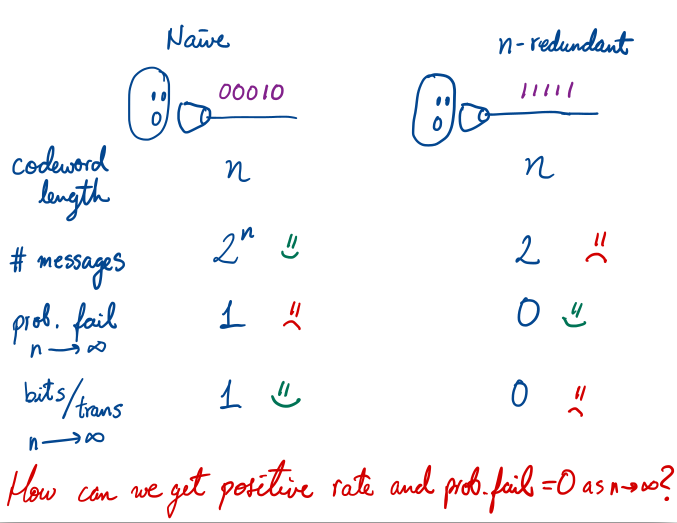
\includegraphics[width=\textwidth]{\dir/comparison_naive_n_redundant.png}
\caption{}
\label{fig:comparison_naive_n_redundant}
\end{figure}

\subsubsection*{Intuition on Shannon's channel coding theorem}

We started by using the binary noisy channel to send bits and we are now devising codes to send a finite set of letters through the binary noisy channel. In a similar manner, we can devise codes to send words through the binary noisy channel, by creating a code that maps words to bit strings of fixed length.\carlos{Why are we talking only of finite sentences $S$? In practice, I want to send sentences of variable lengths. Also, why don't we allow encodings of different lengths?} 

We can continue in this way to create codes to send images of a fixed size, videos of a fixed length, and so on.\carlos{Why the obsession with fixed size?} All this is done by using longer codewords. 

%Observe, however, that the length $n$ of a codeword must be sufficiently large in order to
%%
%\begin{itemize}
%\item have a one-to-one correspondence from messages to codewords\carlos{What's a message?} and
%\item ensure robustness against the channel's noise.
%\end{itemize}
%%
%At the same time, the length $n$ of a codeword must not be too large, as the rate of actual bits of information per tranmission goes to $0$ as $n$ increases.

Shannon's coding theorem concerns with the problem of finding sustainable strategies for building codes. By sustainable, we mean that the strategy should yield codes that fulfill two conditions. 
%
\begin{itemize}
\item First, the codes attain and maintain a positive rate $r$ of bits of information per transmission as $n \to \infty$.
\item Second, the probability of a communication error goes to zero as $n \to \infty$.
\end{itemize}

Shannon's channel coding theorem states that there is a sustainable strategy for building codes, as long as the targeted rate $r$ is below the channel's capacity. For a fixed codeword length $n$, the maximum number of messages that can be communicated with this strategy is $\lfloor 2^{nr}\rfloor$.

\subsubsection*{Formalization}

For the definitions below, let $M, n \in \mathbb{N}$ and let $(\mathfrak{A}, \mathcal{P})$ be a channel.

\begin{definition}
An \emph{$(M, n)$-code} is a pair $(\mathit{Enc}, \mathit{Dec})$ of functions with $\mathit{Enc}: \{1, 2, \ldots, M\} \to \mathfrak{A}^n$ and $\mathit{Dec}: \mathfrak{A}^n \to \{1, 2, \ldots, M\}$.
\end{definition}

\begin{definition}
The \emph{rate of a $(M, n)$-code} is 
%
$$\frac{\log M}{n}.$$
%
\end{definition}

Observe that if a $(M, n)$-code has rate $r$, then $M = 2^{nr}$.

\begin{definition}
For an $(M, n)$-code $(\mathit{Enc}, \mathit{Dec})$,
its \emph{probability of a communication error} is
%
$$\frac{1}{M}\sum_{i \leq M} \prob\left(\mathit{Dec}(\hat{W}) \neq i \mid W = \mathit{Enc}\left(i\right)\right),$$
%
where $\prob\left(\mathit{Dec}(\hat{W}) \neq i \mid W = \mathit{Enc}\left(i\right)\right)$ is the probability that the receiver decodes something different to $i$, given that we sent $\mathit{Enc}\left(i\right)$ through the channel.
\end{definition}

Intuitively, the probability of a communication error is the probability that the receives decodes a wrong message when we send him the codeword of a message chosen uniformly at random.

\begin{example}
The $n$-redundant code discussed above is an example of a $(2^n, n)$-code, whose rate is $\log 2^n / n = 1$.
\end{example}

\begin{definition}
A rate $r$ is \emph{attainable} if there is a sequence of $\left(\lfloor2^{nr}\rfloor, n\right)$-codes, indexed by $n$, such that the probability of a communication error goes to zero as $n \to \infty$.
\end{definition}

\subsection{Shannon's coding theorem}

\subsubsection*{Typicality}

We now recall some important notions from Thomas and Cover~\cite{infotheory}

\begin{theorem}{(The asymptotic equipartition property)} Let $S, S_1$, $S_2, \ldots$, $S_n$ be identically and independently distributed random variables with distribution $p(\cdot)$ over a space $\mathcal{S}$, then
%
$$-\frac{1}{n} p(S_1, \ldots, S_n) \to H(S), \quad \text{in probability as } n \to \infty.$$
%
\end{theorem}

This theorem follows from the weak law of large numbers. In our context, $S, S_1, S_2, \ldots, S_n$ denote symbols from a channel's alphabet and $p(\cdot)$ is $\arg\max_p I(S; \hat{S})$. That is, $p(\cdot)$ is the distribution that achieves the channel's capacity.

\begin{definition}
For $n \in \mathbb{N}$ and $\epsilon > 0$, the \emph{typical set $A^{(n)}_\epsilon$} with respect to $p(\cdot)$ is the set of sequences $(s_1, \dots, s_n) \in \mathcal{S}^n$ such that
%
$$H(S) - \epsilon \leq -\frac{1}{n}\log p(s_1, s_2, \ldots, s_n) \leq H(S) + \epsilon.$$
%
A sequence in $A^{(n)}_\epsilon$ is called a \emph{typical sequence}.
\end{definition}

In our context, codewords will consist of typical sequences.
The next theorem justifies the following intuitions:

\begin{enumerate}
\item All typical sequences have approximately the same probability $\approx 2^{-nH(S)}$.
\item If you draw a sequence in $\mathcal{S}^n$, using $p(\cdot)$, then the resulting sequence is typical with high probability.
\item $\left|A^{(n)}_\epsilon\right| \approx 2^{nH(S)}$.
\end{enumerate}

\begin{theorem}\mbox{   }
\begin{enumerate}
\item If $\left(s_1, s_2, \ldots, s_n\right) \in A^{(n)}_\epsilon$, then $2^{-n\left(H(S) + \epsilon\right)} \leq p(s_1, \ldots, s_n) \leq 2^{-n\left(H(S) - \epsilon\right)}.$
\item $\prob\left(A^{(n)}_\epsilon\right) > 1 - \epsilon$, for sufficiently large $n$.
\item $(1 - \epsilon)2^{n\left(H(S) - \epsilon\right)} \leq \left|A^{(n)}_\epsilon\right| \leq 2^{n\left(H(S) + \epsilon\right)}$.
\end{enumerate}
\end{theorem}

The reader can take it as an exercise to proof these claims. The proofs are in Thomas and Cover~\cite{infotheory}.

\begin{definition}
Let $n \in \mathbb{N}$ and let $p_{S\hat{S}}(\cdot, \cdot)$ be the joint distribution of two random variables $S$ and $\hat{S}$, whose ranges are $\mathcal{S}$ and $\mathcal{\hat{S}}$, respectively. The set $A^{(n)}_\epsilon$ of \emph{jointly typical sequences} with respect to $p_{S\hat{S}}$ is the set of pairs $(\mathbf{s}^n, \hat{\mathbf{s}}^n)$ of sequences that fulfill the following:
%
\begin{enumerate}
\item $\left|-\frac{1}{n}\log p_{S^n}(\mathbf{s}^n) - H(S)\right| < \epsilon$.
\item $\left|-\frac{1}{n}\log p_{\hat{S}^n}(\hat{\mathbf{s}}^n) - H(\hat{S})\right| < \epsilon$.
\item $\left|-\frac{1}{n}\log p_{S^n\hat{S}^n}(\mathbf{s}^n, \hat{\mathbf{s}}^n) - H(S, \hat{S})\right| < \epsilon$.
\end{enumerate}
% 
A pair in $A^{(n)}_\epsilon$ is called a \emph{jointly typical pair of sequences}.
\end{definition}

We clarify that, for $\mathbf{s}^n = (s_1, \ldots, s_n)$ and $\hat{\mathbf{s}}^n = (\hat{s}_1, \ldots, \hat{s}_n)$,
%
$$p_{S^n}(\mathbf{s}^n) = \prod_{i \leq n} p_S(s_i),$$
%
$$p_{\hat{S}^n}(\hat{\mathbf{s}}^n) = \prod_{i \leq n} p_{\hat{S}}(\hat{s}_i) = \prod_{i \leq n} \sum_{s} p_S(s) p_{\hat{S}\mid S}\left(\hat{s}_i \mid s\right), \text{and}$$
%
$$p_{S^n\hat{S}^n}(\mathbf{s}^n, \hat{\mathbf{s}}^n) = \prod_{i \leq n} p_{S\hat{S}}(s_i, \hat{s}_i) = \prod_{i \leq n} p_S(s_i) p_{\hat{S} \mid S}(\hat{s}_i \mid s_i).$$

In the context of communication via a channel, $p_{S^n\hat{S}^n}$ represents the joint distribution of $\mathbf{S}^n$ and $\hat{\mathbf{S}}^n$, where 
%
\begin{itemize}
\item $\mathbf{S}^n$ denotes a random codeword, where each symbol was chosen at random according to the distribution $p_S = \arg \max_p I(S; \hat{S})$ that achieves channel capacity.
\item $\hat{\mathbf{S}}^n$ denotes a codeword that the channel would output, after we send $\mathbf{S}^n$ as input.
\end{itemize}
%
We call $p_{S^n\hat{S}^n}$ the \emph{codeword input-output distribution}.

In the context of communication via a channel, the following theorem justifies the following intuitions:

\begin{enumerate}
\item Suppose that we build a codeword $\mathbf{s}^n$ at random by choosing each of its symbols at random according to $p_S$, the distribution that attains channel capacity. Then we send $\mathbf{s}^n$ through the channel and let $\hat{\mathbf{s}}^n$ be the output codeword. Then $(\mathbf{s}^n, \hat{\mathbf{s}}^n)$ is jointly typical with high probability.
\item Suppose now that we build another codeword ${\mathbf{q}}^n$ at random using the same procedure. Then it is very \emph{unlikely} that $({\mathbf{q}}^n, \mathbf{y}^n)$ is jointly typical.
\end{enumerate}

\begin{theorem}\mbox{  }
\begin{enumerate}
\item $\prob\left(\left(\mathbf{S}^n, \hat{\mathbf{S}}^n\right) \in A^{(n)}_{\epsilon}\right) \to 1$, as $n \to \infty$.
\item If $\mathbf{Q}^n \sim p_{S^n}(\cdot)$ and $\hat{\mathbf{S}}^n \sim p_{\hat{S}^n}(\cdot)$ (i.e., they are drawn independently at random from the marginal distributions of $p_{S^n\hat{S}^n}$), then
%
$$(1-\epsilon)2^{-n\left(I(S;\hat{S}) + 3\epsilon\right)} \leq \prob\left(\left({\mathbf{Q}}^n, \hat{\mathbf{S}}^n\right) \in A^{(n)}_{\epsilon}\right) \leq 2^{-n\left(I(S;\hat{S}) - 3\epsilon\right)}$$
%
\end{enumerate}
\label{thm:joint_typical}
\end{theorem}

These two intuitions justify the effectiveness of a very simple code, called \emph{Shannon's random code}. 

\subsubsection*{Shannon's random code}

\begin{theorem}
A rate is attainable iff it is below the channel's capacity.
\end{theorem}

We only focus here on proving the following direction: if a rate is below the channel's capacity, then it is attainable, as it illustrates how to propose a $(\lfloor 2^{nr} \rfloor, n)$-code for communicating $\lfloor 2^{nr} \rfloor$ messages.

To prove this, we present, for $n > 1$, a $(\lfloor 2^{nr}\rfloor, n)$-code whose probability of a communication error is at most $p_n = 2^{-n\left(\mathit{cap} - 3\epsilon - r\right)}$, where $\epsilon$ is chosen to be sufficiently small. Hence, if $r < \mathit{cap}$, we get that the probability of a communication error goes to zero as $n \to \infty$.

The code's encoder function $\mathit{Enc}$ is defined as follows. For a message $m \leq \lfloor 2^{nr}\rfloor$, we define $\mathit{Enc}(m)$ as a string in $\mathbf{s}^n$ where each symbol was drawn from a distribution $p^* = \arg\max_{p(\cdot)} I(S; \hat{S})$. That is, a distribution that maximizes the channel's input-output mutual information and attains the channel's capacity.

The code's decoder function $\mathit{Dec}$ is defined as follows. Given the string $\mathbf{s}^n$ output by the channel, $\mathit{Dec}$ goes through each message $m$ and tests if $(\mathit{Enc}(m), \mathbf{s}^n)$ is jointly typical with respect to the codeword input-output distribution $p_{S^n\hat{S}^n}$. $\mathit{Dec}$ outputs the first message for which this test succeeds. If no message succeeds on the test, then $\mathit{Dec}$ outputs an arbitrary message.

\carlos{Remind the reader that the sender and the receiver agree in advance on $\mathit{Enc}$ and $\mathit{Dec}$. Therefore, the receiver also knows both $\mathit{Enc}$ and the set $\{1, 2, \ldots, \lfloor 2^{nr}\rfloor$ of messages.}

\begin{theorem}
The probability $\prob\left(\mathcal{E}\right)$ of a communication error for Shannon's random code goes to 0 as $n \to \infty$.
\label{thm:shannon_random_code}
\end{theorem}

\begin{proof}
Let $\mathcal{K}$ be a random variable representing a possible code. Then
%
$$\prob\left(\mathcal{E}\right) = \sum_{\mathcal{K}} \prob\left(\mathcal{K}\right) P_e(\mathcal{K}),$$
%
where $P_e(\mathcal{K})$ is the probability of a communication error for code $\mathcal{K}$. Observe now that
%
\begin{align*}
\prob\left(\mathcal{E}\right) &= \sum_{\mathcal{K}} \prob\left(\mathcal{K}\right) P_e(\mathcal{K})\\
&= \sum_{\mathcal{K}} \prob\left(\mathcal{K}\right) \frac{1}{\lfloor 2^{nr}\rfloor}\sum_{w \leq \lfloor 2^{nr}\rfloor} \prob\left(\mathit{Dec}(\hat{\mathbf{S}}^n) \neq w \mid \mathbf{S}^n = \mathit{Enc}(w)\right)\\
&= \frac{1}{\lfloor 2^{nr}\rfloor} \sum_{\mathcal{K}} \sum_{w \leq \lfloor 2^{nr}\rfloor} \prob\left(\mathcal{K}\right)  \prob\left(\mathit{Dec}(\hat{\mathbf{S}}^n) \neq w \mid \mathbf{S}^n = \mathit{Enc}(w)\right).
\end{align*}

Observe now that all codewords were chosen independently at random, so 
%
$$\prob\left(\mathit{Dec}(\hat{\mathbf{S}}^n) \neq w \mid \mathbf{S}^n = \mathit{Enc}(w)\right) = \prob\left(\mathit{Dec}(\hat{\mathbf{S}}^n) \neq 1 \mid \mathbf{S}^n = \mathit{Enc}(1)\right),$$ 
%
for $w > 1$. Hence,
%
\begin{align*}
\prob\left(\mathcal{E}\right) &= \frac{1}{\lfloor 2^{nr}\rfloor} \sum_{\mathcal{K}} \sum_{w \leq \lfloor 2^{nr}\rfloor} \prob\left(\mathcal{K}\right)  \prob\left(\mathit{Dec}(\hat{\mathbf{S}}^n) \neq w \mid \mathbf{S}^n = \mathit{Enc}(w)\right)\\
&= \sum_{\mathcal{K}} \prob\left(\mathcal{K}\right)  \prob\left(\mathit{Dec}(\hat{\mathbf{S}}^n) \neq 1 \mid \mathbf{S}^n = \mathit{Enc}(1)\right)\\
&= \prob\left(\mathcal{E} \mid w = 1\right).
\end{align*}

This means that the probability of a communication error is equal to the probability of a communication error, assuming that the sender sent the codeword for message 1.

Note that, in Shannon's random code, the event of a communication error implies at least one of the following events: the received codeword $\hat{\mathbf{S}}^n(1)$ is not jointly typical with the codeword $\mathbf{S}^n(1)$ for message 1 or the received codeword $\hat{\mathbf{S}}^n(1)$ is jointly typical with the codeword $\mathbf{S}^n(w)$ for a message $w > 1$. More precisely,
%
\begin{align*}
\prob\left(\mathcal{E} \mid M = 1\right) &= \prob\left(
\begin{array}{c}
\left(\mathbf{S}^n(1), \hat{\mathbf{S}}^n(1)\right) \notin A^{(n)}_{\epsilon} \; \text{or}\\
\left(\mathbf{S}^n(2), \hat{\mathbf{S}}^n(1)\right) \in A^{(n)}_{\epsilon} \; \text{or}\\
\left(\mathbf{S}^n(3), \hat{\mathbf{S}}^n(1)\right) \in A^{(n)}_{\epsilon} \; \text{or}\\
\vdots\\
\left(\mathbf{S}^n(\lfloor2^{nr}\rfloor), \hat{\mathbf{S}}^n(1)\right) \in A^{(n)}_{\epsilon}.
\end{array}
\right).
\end{align*}
%
By the union bound,
%
$$\prob\left(\mathcal{E} \mid M = 1\right) \leq \prob\left(\left(\mathbf{S}^n(1), \hat{\mathbf{S}}^n(1)\right) \notin A^{(n)}_{\epsilon}\right) + \sum_{w > 1}\prob\left(\left(\mathbf{S}^n(w), \hat{\mathbf{S}}^n(1)\right) \in A^{(n)}_{\epsilon}\right).$$
%
We now apply Theorem~\ref{thm:joint_typical}, which implies the following:

\begin{itemize}
\item $\prob\left(\left(\mathbf{S}^n(1), \hat{\mathbf{S}}^n(1)\right) \notin A^{(n)}_{\epsilon}\right) \to 1$, as $n \to \infty$. In other words, $\prob\left(\left(\mathbf{S}^n(1), \hat{\mathbf{S}}^n(1)\right) \notin A^{(n)}_{\epsilon}\right) \to 0$, as $n \to \infty$.
\item $\prob\left(\left(\mathbf{S}^n(w), \hat{\mathbf{S}}^n(1)\right) \in A^{(n)}_{\epsilon}\right) \leq 2^{-n\left(I(S;\hat{S})-3\epsilon\right)}$. This is because, for $w > 1$, $\mathbf{S}^n(1)$ and $\mathbf{S}^n(w)$ were independently drawn from $p_{S^n}$ and, therefore, $\hat{\mathbf{S}}^n(1)$ and $\mathbf{S}^n(w)$ were independently drawn from $p_{\hat{S}^n}$ and $p_{S^n}$, respectively.
\end{itemize}

Using these observations we get that
%
\begin{align*}
\prob\left(\mathcal{E} \mid M = 1\right) &\leq \prob\left(\left(\mathbf{S}^n(1), \hat{\mathbf{S}}^n(1)\right) \notin A^{(n)}_{\epsilon}\right) + \sum_{w > 1}\prob\left(\left(\mathbf{S}^n(w), \hat{\mathbf{S}}^n(1)\right) \in A^{(n)}_{\epsilon}\right)\\
&\leq \prob\left(\left(\mathbf{S}^n(1), \hat{\mathbf{S}}^n(1)\right) \notin A^{(n)}_{\epsilon}\right) + \sum_{w > 1} 2^{-n\left(I(S;\hat{S}) - 3\epsilon\right)}\\
&= \prob\left(\left(\mathbf{S}^n(1), \hat{\mathbf{S}}^n(1)\right) \notin A^{(n)}_{\epsilon}\right) + \left(\lfloor 2^{nr}\rfloor - 1\right)2^{-n\left(I(S;\hat{S}) - 3\epsilon\right)}\\
&\leq \prob\left(\left(\mathbf{S}^n(1), \hat{\mathbf{S}}^n(1)\right) \notin A^{(n)}_{\epsilon}\right) + 2^{nr} 2^{-n\left(I(S;\hat{S}) - 3\epsilon\right)}\\
&= \prob\left(\left(\mathbf{S}^n(1), \hat{\mathbf{S}}^n(1)\right) \notin A^{(n)}_{\epsilon}\right) + 2^{-n\left(I(S;\hat{S}) - r - 3\epsilon\right)}.
\end{align*}
%

Observe that we chose $p_S$ as $\arg\max_p I(S;\hat{S})$, so $I(S;\hat{S}) = \mathit{cap}$, the channel's capacity. So, if the rate $r$ is below the channel's capacity and $\epsilon$ is sufficiently small, then $\prob\left(\mathcal{E} \mid M = 1\right) \to 0$ as $n \to \infty$.
\end{proof}

\section{Communication protocol for algorithm validation}
\label{sec:comm_protocol}

We now formalize the communication protocol where posterior agreement originates. We first explain an \emph{ideal variant} where we know $X$'s probability distribution $p_X$. Furthermore, we assume that $p_X$ is from a parameterized family $\mathfrak{P}$ of probability distributions. Afterwards, we explain the \emph{empirical variant} where we do not know anything about $p_X$ and, even worse, we only have \emph{two observations} $X'$ and $X''$ drawn from $p_X$. Recall that, in practice, we only have access to observations and have no information of the nature of the distribution where these observations came from.\looseness=-1

\subsection{Assumptions}

For our statements to hold, we make the following assumptions.

\paragraph{Exponential solution space:} We assume that $\mathcal{C}$ is discrete and that $\log \left|\mathcal{C}\right| = \Theta(n)$, where $n$ measures the ``size'' of an observation from a phenomenon. For example, $n$ measures the number of edges in a graph or the number of datapoints in a clustering instance. Intuitively, we assume that the solution space's size grows exponentially in $n$.

\paragraph{Probabilistic outputs:} We assume that any algorithm for stochastic optimization, when given an input $X'$ from an instance space $\mathcal{X}$, outputs a distribution $p(\cdot \mid X')$ over a discrete solution space $\mathcal{C}$. Every algorithm can be thought to be as such, even when it only outputs a fixed value $c_{X'} \in \mathcal{C}$, when given $X'$ as input. In this case, $p(c \mid X') = 1$ if $c = c_{X'}$ and $0$ otherwise.

\subsection{Ideal variant}

Let $\mathcal{A}$ be an algorithm intended for solving Problem~\ref{eq:stoch_min_span_tree}. Posterior agreement originates from a communication protocol between a sender and a receiver. The sender must communicate, using $\mathcal{A}$'s outputs, the nature of a phenomenon to the receiver. The receiver must be able, using the information sent from the sender, to identify the phenomenon. The communication from the sender to the receiver is done through a noisy channel, whose noise is defined by $\mathcal{A}$ and the phenomenon.

\paragraph{Messages} Fix $n \in \mathbb{N}$. Present the instance space $\mathcal{X}$ to the sender and the receiver. Then agree draw at random a set $\mathcal{F} \subseteq \mathfrak{P}$ of $m$ phenomena and, for each $p_i \in \mathcal{F}$, draw an observation $X'_i$ of size $n$. Let $\mathcal{M} = \{X'_1, \ldots, X'_m\}$. Agreeing on $\mathcal{F}$ is often not possible in practice, so we explain in the empirical variant how to deal with this. This $\mathcal{M}$ constitutes the set of possible messages that the sender may try to communicate to the receiver.

For the moment, we leave the value of $m$ undefined. We leave for later to figure out what is the maximum value of $m$ that we can use. The choice of $m$ must still ensure that the probability of a communication error goes to 0, as $n \to \infty$.

\paragraph{Code} Present algorithm $\mathcal{A}$ to the sender and the receiver. For each $X' \in \mathcal{M}$, use $\mathcal{A}$ to compute $p(\cdot \mid X')$. Define the code $(\mathit{Enc}_{\mathcal{A}}, \mathit{Dec}_{\mathcal{A}})$ as follows:

\begin{itemize}
\item $\mathit{Enc}_{\mathcal{A}}$ encodes $X' \in \mathcal{M}$ as the codeword $p(\cdot \mid X')$.
\item $\mathit{Dec}_{\mathcal{A}}$ decodes a probability distribution $p(\cdot \mid Y)$ over $\mathcal{C}$ as any $\hat{X} \in \mathcal{M}$ such that $\kappa\left(Y, \hat{X}\right) \geq \kappa\left(Y, X\right)$, for all $X \in \mathcal{M}$. Here,
%
$$\kappa\left(Y, X'\right) := \sum_c p(c \mid Y)p(c \mid X').$$
%
\end{itemize}

\paragraph{Channel} The channel is the pair $\left(\left\{p(\cdot \mid X')\right\}_{X' \in \mathcal{M}}, \mathcal{P}\right)$ where $\mathcal{P}$ is defined by the following probabilistic procedure. Assume that the sender inputs $p(\cdot \mid X')$ to the channel. The channel then replaces $X'$ with a fresh new observation $X''$ from the same phenomenon where $X'$ comes from. Then it uses the algorithm $\mathcal{A}$ to compute $p(\cdot \mid X'')$ and outputs that to the receiver.

\paragraph{Communication} A message $X'$ is selected uniformly at random from $\mathcal{M}$ and without the receiver's knowledge. The sender then sends the codeword $p(\cdot \mid X')$ through the channel. The receiver gets $p(\cdot \mid X'')$ and uses the decoding function to guess which message the sender sent. The receiver succeeds by correctly guessing $X'$.

Observe how the algorithm and the phenomenon define the channel's noise. Hence, the algorithm can be evaluated by \emph{the capacity} of the resulting channel. This capacity is measured by its maximum attainable rate, which is obtained by figuring out how to maximize the number $m$ of messages that can be used in the protocol, while making the probability of a communication error go to zero as $n$, the size of the observations, go to infinity. We carry this analysis in the empirical variant.

\subsection{Empirical variant}

The capacity of the channel built above cannot be computed, as we often only have access to a set of observations and not to the phenomena behind them. This means that we cannot compute the set $\mathcal{M}$ of messages, as described in the ideal variant. For this reason, we use an empirical variant, where we assume that we are given at least two observations $X'$ and $X''$ of a same phenomenon.

\paragraph{Messages} (Figure~\ref{fig:agree_on_trans}) We create a set of messages by producing \emph{transformed copies} of $X'$. We take a set $\mathbb{T}$ of transformations, where each transformation transforms instances into instances. Afterwards, we draw $m$ transformations  $\tau_1, \tau_2, \ldots, \tau_m$ from $\mathbb{T}$ uniformly at random. In this way, we can create a set $\mathcal{M} = \left\{\tau_1 \circ X', \tau_2 \circ X', \ldots, \tau_m \circ X'\right\}$ of messages that are analogous to the set of messages that we created in the ideal variant. We impose the following requirements on $\mathbb{T}$ so that $\mathcal{M}$ looks like the set $\mathcal{M}$ that we would obtain in the ideal variant.

\begin{itemize}
\item $\sum_{\tau} p(c \mid \tau \circ X') \in \left[\frac{\left|\mathbb{T}\right|}{\left|\mathcal{C}\right|}(1 - \rho), \frac{\left|\mathbb{T}\right|}{\left|\mathcal{C}\right|}(1 + \rho)\right]$, for some small $\rho > 0$. The reason for this assumption is that we we do not want the probability mass of all these codewords to be concentrated in a narrow subset of $\mathcal{C}$, as this reduces the number of different messages that the sender can communicate to the receiver. This ensures that, for each $c \in \mathcal{C}$, the total probability mass $c$ gets is $\sum_{\tau} p(c \mid \tau \circ X') \approx \frac{\left|\mathbb{T}\right|}{\left|\mathcal{C}\right|}$.
\item The transformations do not alter an instance's randomness. 
%\item For any $\tau_1, \tau_2 \in \mathbb{T}$, $\left|p(\cdot \mid \tau_1 \circ X') - p(\cdot \mid \tau_2 \circ X'')\right| > 0$. That is, different transformations should induce different codewords.
\end{itemize}

Observe that such a set of transformations does not necessarily always exist. For example, if the algorithm under evaluation always produces the same constant distribution $p(\cdot \mid X')$, independent of $X'$, then no set of transformations will be able to achieve the requirement above. In this case, however, there is no need to build a channel to evaluate such an algorithm, as it is clear that the algorithm is not producing any value from the data.

\begin{figure}
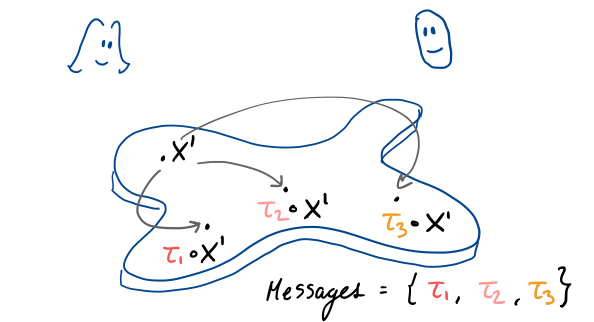
\includegraphics[width=\textwidth]{\dir/agree_on_trans.png}
\caption{}
\label{fig:agree_on_trans}
\end{figure}

\paragraph{Code} (Figure~\ref{fig:emp_agree_on_code}) The encoding and decoding functions are the analogous of the ideal variant. The codeword of a message $\tau \in \mathcal{M}$ is $p(\cdot \mid \tau \circ X')$. When given a codeword $p(\cdot \mid Y)$, the decoding function outputs the message $\tau$ for which $\kappa\left(Y, \tau \circ X'\right) \geq \kappa\left(Y, \sigma \circ X'\right)$, for every $\sigma \in \mathcal{M}$.

\begin{figure}
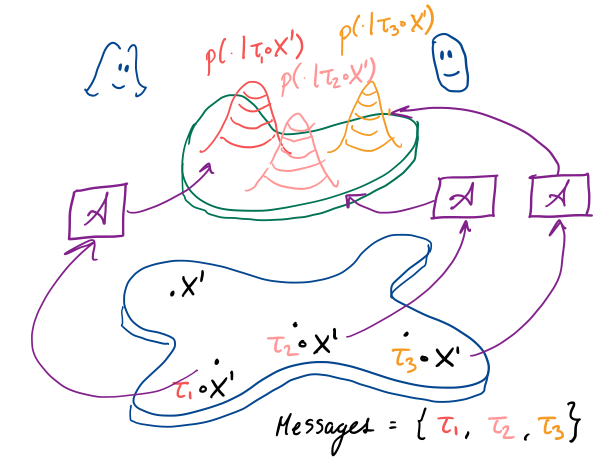
\includegraphics[width=\textwidth]{\dir/emp_agree_on_code.png}
\caption{}
\label{fig:emp_agree_on_code}
\end{figure}

\paragraph{Channel} (Figure~\ref{fig:send_codeword}) When the sender inputs $p(\cdot \mid \tau \circ X')$ to the channel, the channel outputs $p(\cdot \mid \tau \circ X'')$, as in the ideal variant.

\begin{figure}
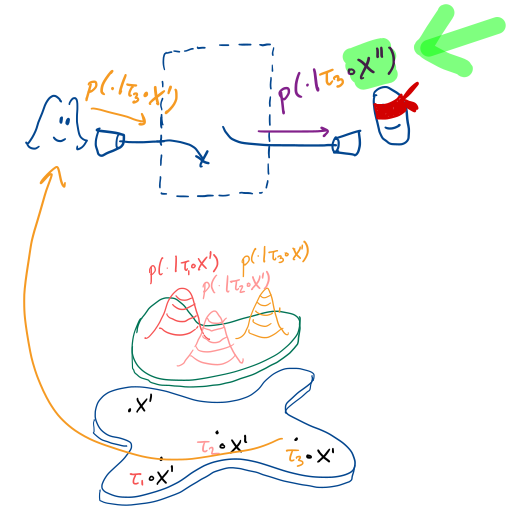
\includegraphics[width=\textwidth]{\dir/send_codeword.png}
\caption{}
\label{fig:send_codeword}
\end{figure}

\paragraph{Protocol} The sender and the receiver agree on a set $\mathbb{T}$ of transformations and use the algorithm under evaluation $\mathcal{A}$ to compute the code's encoding and decoding functions. A set $\mathcal{M} = \left\{\tau_1, \ldots, \tau_m\right\}$ of $m$ messages is drawn uniformly at random from $\mathbb{T}$. A message $\tau \in \mathcal{M}$ is selected uniformly at random and without the receiver's knowledge. The sender then sends the codeword $p(\cdot \mid \tau \circ X')$ through the channel. The receiver gets $p(\cdot \mid \tau \circ X'')$ and uses the decoding function to guess which message the sender sent (Figure~\ref{fig:guessing}). The receiver succeeds by correctly guessing $\tau$.

\begin{figure}
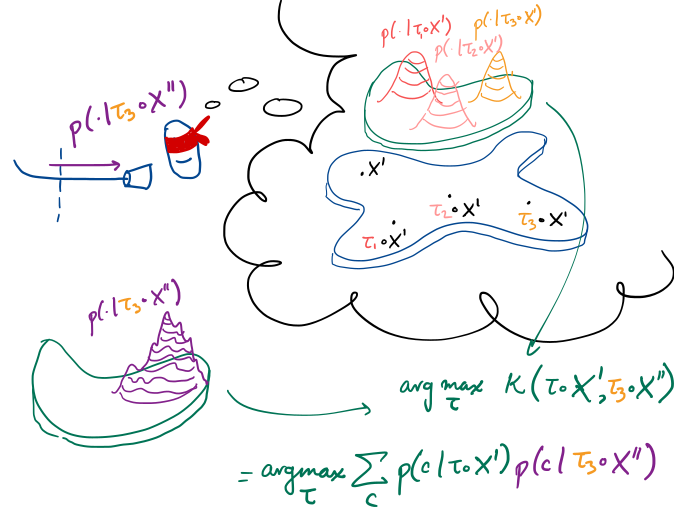
\includegraphics[width=\textwidth]{\dir/emp_guessing.png}
\caption{}
\label{fig:emp_guessing}
\end{figure}

\subsection{Probability of a communication error}
\label{sub:prob_comm_error}

\begin{theorem}
The probability of a communication error is bounded above by 
%
\begin{equation}
P_{(n)} = \exp\left(- I + \log m + \epsilon \log\left|\mathcal{C}\right|\right),
\label{eq:prob_comm_error_empirical_var}
\end{equation}
%
where
%
\begin{equation}
I := \mathbb{E}_{X', X''}\left[\log \left(\left|\mathcal{C}\right|k(X', X'')\right)\right]
\label{eq:exp_log_pa}
\end{equation}
%
\label{thm:comm_error_emp_var}
\end{theorem}

One can show that $P_{(n)} \to 0$ as $n \to \infty$ by choosing $\epsilon$ sufficiently small and ensuring that $I - \log m = \Omega(n)$.

\begin{proof}
Let $\tau_s$ be the message sent by the sender and let $\hat{\tau}$ be the message guessed by the receiver. Just as in the proof of Theorem~\ref{thm:shannon_random_code}, one can show that $\prob\left(\hat{\tau} \neq \tau_s\right) = \prob\left(\hat{\tau} \neq \mathit{id}\right)$, where $\mathit{id}$ is some arbitrary transformation. Without loss of generality, we assume that $\mathit{id}$ is the identity transformation.

Using the definition of communication error, we get that
%
$$\prob\left(\hat{\tau} \neq \mathit{id}\right) = \prob\left(\max_{\tau \neq \mathit{id}} \kappa\left(\tau\circ X', X''\right) \geq \kappa\left(X', X''\right) \mid \mathit{id}\right).$$
%
Applying the union bound, we get
%
$$\prob\left(\hat{\tau} \neq \mathit{id}\right) \leq \sum_{\tau \neq \mathit{id}}\prob\left(\kappa\left(\tau\circ X', X''\right) \geq \kappa\left(X', X''\right) \mid \mathit{id}\right).$$
%
We now rewrite probabilities as expectations
%
\begin{align*}
\prob\left(\hat{\tau} \neq \mathit{id}\right) &\leq \sum_{\tau \neq \mathit{id}}\prob\left(\kappa\left(\tau\circ X', X''\right) \geq \kappa\left(X', X''\right) \mid \mathit{id}\right)\\
&= \sum_{\tau \neq \mathit{id}}\mathbb{E}_{X', X''}\left[\mathbb{E}_{\tau}\left[\mathbb{I}\left\{\kappa\left(\tau\circ X', X''\right) \geq \kappa\left(X', X''\right)\right\} \mid \mathit{id}, X', X''\right]\right]\\
&= \sum_{\tau \neq \mathit{id}}\mathbb{E}_{X', X''}\left[\prob\left(\kappa\left(\tau\circ X', X''\right) \geq \kappa\left(X', X''\right) \mid \mathit{id}, X', X''\right)\right].
\end{align*}
%
Here, $\mathbb{I}$ is the indicator function.

We now apply Markov's inequality.
%
\begin{align*}
\prob\left(\hat{\tau} \neq \mathit{id}\right) &\leq \sum_{\tau \neq \mathit{id}}\mathbb{E}_{X', X''}\left[\prob\left(\mathbb{I}\left\{\kappa\left(\tau\circ X', X''\right) \geq \kappa\left(X', X''\right)\right\} \mid \mathit{id}, X', X''\right)\right]\\
&\leq \sum_{\tau \neq \mathit{id}}\mathbb{E}_{X', X''}\left[\frac{\mathbb{E}_\tau\left[\kappa\left(\tau \circ X', X''\right) \mid \mathit{id}, X', X'' \right]}{\kappa\left(X', X''\right)}\right].
\end{align*}
%

We now compute an upper bound for the numerator.
%
\begin{align*}
\mathbb{E}_\tau \left[\kappa\left(\tau \circ X', X''\right) \mid X', X''\right]
&= \mathbb{E}_\tau \left[\sum_c p(c \mid \tau \circ X') p(c \mid X'') \mid X', X''\right]\\
&= \sum_c p(c \mid X'') \mathbb{E}_\tau \left[p(c \mid \tau \circ X')\right]\\
&= \sum_c p(c \mid X'') \sum_\tau \frac{1}{\left|\mathbb{T}\right|} p(c \mid \tau \circ X')\\
&\leq \frac{1}{\left|\mathbb{T}\right|}\frac{\left|\mathbb{T}\right|}{\left|\mathcal{C}\right|}(1 + \rho)\sum_c p(c \mid X'') = (1 + \rho)\frac{1}{\left|\mathcal{C}\right|}.
\end{align*}
%
For the last inequality, we used the assumption that $\sum_{\tau} p(c \mid \tau \circ X') \in \left[\frac{\left|\mathbb{T}\right|}{\left|\mathcal{C}\right|}(1 - \rho), \frac{\left|\mathbb{T}\right|}{\left|\mathcal{C}\right|}(1 + \rho)\right]$.

We have then that
%
\begin{align*}
\prob\left(\hat{\tau} \neq \mathit{id}\right) &\leq \sum_{\tau \neq \mathit{id}} \mathbb{E}_{X', X''}\left[\frac{1 + \rho}{\left|\mathcal{C}\right|\kappa\left(X', X''\right)}\right]\\
&= (1 + \rho)\left(m - 1\right) \mathbb{E}_{X', X''}\exp\left(-\log\left(\left|\mathcal{C}\right|\kappa\left(X', X''\right)\right)\right)\\
&\leq m (1 + \rho) \; \mathbb{E}_{X', X''}\exp\left(-\log\left(\left|\mathcal{C}\right|\kappa\left(X', X''\right)\right)\right)\\
&= (1 + \rho)\mathbb{E}_{X', X''}\exp\left(-\log\left(\left|\mathcal{C}\right|\kappa\left(X', X''\right)\right) + \log m\right)\\
&\approx \; \mathbb{E}_{X', X''}\exp\left(-\hat{I} + \log m\right).
\end{align*}
%
Here, for simplicity, we assumed $1 + \rho \approx 1$.

To provide an upper bound to $\prob\left(\hat{\tau} \neq \mathit{id}\right)$, we must bound the behavior of the random variable $\hat{I} = \log\left(\left|\mathcal{C}\right|\kappa\left(X', X''\right)\right)$. To do this, we assume that $\hat{I}$ satisfies \emph{an asymptotic equipartition property} in the sense that, as $n \to \infty$, $\hat{I} \to I$, where $I = \mathbb{E}_{X', X''}\log\left(\left|\mathcal{C}\right|\kappa\left(X', X''\right)\right)$, the expected log posterior agreement. Under this assumption, for every $\epsilon, \delta > 0$, there is $n_0 \in \mathbb{N}$ such that for any $n > n_0$,
%
$$\prob\left(\left|\hat{I} - I\right| \leq \epsilon \log \left|\mathcal{C}\right|\right) > 1 - \delta.$$
%

\todo{Explain why this assumption is reasonable. In particular, explain its connection to typicality.}

With this assumption, we can derive the following:
%
\begin{align*}
\prob\left(\hat{\tau} \neq \mathit{id}\right) &\leq \mathbb{E}_{X', X''}\exp\left(-\hat{I} + \log m\right)\\
&= \mathbb{E}_{X', X''}\exp\left(-\hat{I} + (I-I) + \log m\right)\\
&= \mathbb{E}_{X', X''}\exp\left(-I + (I - \hat{I}) + \log m\right)\\
&\leq \mathbb{E}_{X', X''}\exp\left(-I + \left|I - \hat{I}\right| + \log m\right)\\
&\leq \mathbb{E}_{X', X''}\exp\left(-I + \epsilon \log \left|\mathcal{C}\right| + \log m\right)\\
&= \exp\left(-I + \epsilon \log \left|\mathcal{C}\right| + \log m\right).
\end{align*}
%
This concludes the proof.
\end{proof}

Recall that the goal is to be able to maximize the number of distinguishable messages that can be sent through the channel. Hence, we must aim to make both $m$ and $I$ as large as possible. The algorithm can only influence $I$ and, therefore, good algorithms \emph{shall maximize the expected log posterior agreement}.

Computing $I$ requires the underlying distribution of $X'$ and $X''$, which we assume to be unknown. In this case, we can approximate $I$ with \emph{the empirical log posterior agreement}
%
\begin{equation}
\frac{1}{L}\sum_{\ell \leq L} \left[\log \left(\left|\mathcal{C}\right|k(X'_\ell, X''_\ell)\right)\right],
\label{eq:emp_log_pa}
\end{equation}
%
where $\left\{X'_1, X''_1, \ldots, X'_L, X''_L\right\}$ is a set of observations.

Finally, we remark some analogies with Shannon's channel coding theorem. The quantity $\frac{1}{n}\mathbb{E}_{X', X''}\log\left(\left|\mathcal{C}\right|\kappa\left(X', X''\right)\right)$ plays the role the input-output mutual information. The value $\log m / n$ plays the role of the code rate.
%
%\section{Applications}
%
%\subsection{Validating stopping temperatures}
%
%In the statistical learning theory course, we learned about algorithms like deterministic annealing, which use maximum-entropy approaches to estimate $\min_c \mathbb{E}\left[R(c, X)\right]$, for a given cost function $R(\cdot, \cdot)$ and from a given dataset $X'$. These algorithms work by computing the posterior distribution
%%
%$$p_T(c \mid X) \propto \exp\left(-\frac{1}{T}R(c, X')\right).$$
%%
%Here, $T > 0$ is a \emph{temperature} hyper-parameter that defines the distribution's ``width''. Figure~\ref{fig:temp_influences_post_width}\carlos{Figure} illustrates how the temperature influences the posterior's width. Observe the following:
%
%\begin{itemize}
%\item For any two $c_1, c_2 \in \mathcal{C}$, if $R(c_1, X') \leq R(c_2, X')$, then $p(c_1 \mid X') \geq p(c_2 \mid X')$.
%\item When $T \to \infty$, the posterior becomes the uniform distribution over $\mathcal{C}$.
%\item When $T \to 0$, the posterior becomes the uniform distribution over $R(\cdot, X')$'s global minima.
%\end{itemize}
%
%The posterior becomes then a distribution where, for $c \in \mathcal{C}$, the probability $p(c \mid X')$ indicates how much the algorithm believes $c$ to be the solution of $\min_c \mathbb{E}\left[R(c, X)\right]$. However, how can we establish the value for $T$? Posterior agreement offers us an answer. First, get another instance $X''$ from the same source used to obtain $X'$. Then choose
%%
%$$T^* = \arg\max_T \kappa_T\left(X', X''\right) = \arg\max_T \sum_c p_T(c \mid X')p_T(c \mid X'').$$
%%
%\subsection{Validating cost functions}
%
%Posterior agreement also offers us a way to choose among a set of candidate cost functions $R_1(\cdot, \cdot)$, $R_2(\cdot, \cdot), \ldots$, $R_s(\cdot, \cdot)$. The best cost function is the one that maximizes the expected log posterior agreement:
%%
%$$\max_{\ell \leq s} \kappa_\ell\left(X', X''\right) = \max_{\ell \leq s} \frac{1}{Z_{X'}Z_{X''}}\sum_c \exp\left(-\frac{1}{T}R_\ell(c, X')\right)\exp\left(-\frac{1}{T}R_\ell(c, X'')\right),$$
%%
%where $Z_{X'}$ and $Z_{X''}$ are the normalization constants of $p(\cdot \mid X')$ and $p(\cdot \mid X'')$, respectively.
%
%\subsection{Validating algorithms}
%
%Finally, the approach can be extended to algorithms. We present here some analysis conducted by Alexey Gronskiy in his doctorate studies~\cite{??}.
%
%We consider three popular algorithms for computing minimum spanning trees: Prim's, Kruskal's, and reverse-delete. The three algorithms work iteratively. At each iteration $t$, the algorithm computes a set $\mathcal{C}_t$ of candidate spanning trees such that $\mathcal{C} = \mathcal{C}_0 \supseteq \mathcal{C}_1 \supseteq \ldots \supseteq \mathcal{C}_z = \{\hat{c}\}$, where $\hat{c}$ is the empirical risk minimizer of the input $X'$. That is, $\hat{c}$ is the minimum spanning tree of $X'$. We call such algorithms \emph{contractive} as at each iteration, they reduce the set of candidate solutions. 
%
%The three algorithms differ on the sets they compute at each iteration\carlos{Figure illustrating this}. We can assume that the algorithm computes at each iteration $t$ a \emph{posterior distribution} $p_t(\cdot \mid X')$, which is the uniform distribution over $\mathcal{C}_t$. We can therefore convert the algorithm into an algorithm that receives an additional input $z$ that fixed the maximum number of iterations that the algorithm can perform. The output is then a posterior distribution $p_z(\cdot \mid X')$ over spanning trees.
%
%The optimal value for $z^*$ can be established with posterior agreement. Moreover, we can compare these three algorithms using posterior agreement! In his experiments, Gronskiy shows that the reverse-delete algorithm attains a higher empirical log posterior agreement. 
%
%\carlos{To be continued...}
%
%\section{Illustrative example}
%
%Section 3.6 of Alex's thesis.
%
%\todo{Argue why it is computationally feasible to compute $t^* = \arg\max_t \hat{I}^\mathcal{A}\left(X', X''\right)$.}
%
%Observe how posterior agreement tells us, without any previous knowledge of how these algorithms work, which MST algorithm is the most suitable for computing the minimum spanning tree in the presence of noise.
%
%\section{Exercises}
%
%Show that the noisy typewriter channel's capacity with $\epsilon = 0.5$ has capacity $-1 + \log 26$.
%
%Details on Shannon's channel coding theorem's proof.
%
%Posterior agreement for the best value for ridge regression! \todo{exam question?}

% https://www.graphsketch.com/?eqn1_color=1&eqn1_eqn=&eqn2_color=2&eqn2_eqn=3%20%2B%20sin(((1*pi)%2F5)*x%20-%206.2)&eqn3_color=3&eqn3_eqn=&eqn4_color=4&eqn4_eqn=10%20%2B%20sin(((2*pi)%2F5)*x%20-%20(2%20*pi)%2F5%20-%200.25)&eqn5_color=5&eqn5_eqn=&eqn6_color=6&eqn6_eqn=&x_min=-1&x_max=15&y_min=-1&y_max=15&x_tick=1&y_tick=1&x_label_freq=5&y_label_freq=5&do_grid=0&do_grid=1&bold_labeled_lines=0&bold_labeled_lines=1&line_width=4&image_w=850&image_h=525

\bibliographystyle{abbrv}
\bibliography{main}

\appendix

\chapter{Information theory}

To be done in 2022.

\renewcommand{\dir}{em_algorithm}
\chapter{The EM-algorithm}

\newcommand{\timedomain}{[0, \infty)}

\section{Introduction}

We motivate and present the EM (expectation-maximization) algorithm, an algorithm used for approximately computing parameter values for probability distributions in maximum-likelihood estimation. The reader is expected to have knowledge of undergraduate probability theory and to be familiar with maximum-likelihood estimation.

The presentation is divided in three parts. Section~\ref{sec:vegan_flea} presents an optimization problem regarding a vegan flea. We present an algorithm that finds an approximate solution and provides intuitions to understand why the EM-algorithm works. Section~\ref{sec:movie_recommendation} presents the problem of building a simple movie recommendation system. We show that movie ratings can be understood as samples from a probabilistic model that is defined by a set of multivariate Bernoulli distributions. Estimating the parameters of these distributions via maximum-likelihood turns out to be very hard using analytical methods. In Section~\ref{sec:em_algo}, we show that this maximum-likelihood estimation problem is an instance of the vegan-flea optimization problem and derive the EM-algorithm from the approximation algorithm presented in Section~\ref{sec:vegan_flea}.

\section{The vegan-flea optimization problem}
\label{sec:vegan_flea}

\subsection{The dog}

We introduce a two-dimensional dog, depicted in Figure~\ref{fig:dog}. Although, in practice, dogs are three-dimensional entities, a two-dimensional dog makes easier the presentation of some ideas later. Observe that this two-dimensional dog has only two legs, since two legs suffice to keep balance, and one eye, since there is no need for perspectives in a two-dimensional space. 

Figure~\ref{fig:dog_close_up} shows some of the dog's cardiovascular system. Observe that a blood vessel of a two-dimensional being does not have the shape of a cilinder. They still naturally expand when a surge of blood flows from a heart's pump. For the rest of these notes we focus only on a small area of this figure; namely, the tiny green square shown in the figure.

\begin{figure}
\centering
\begin{subfigure}[b]{0.45\textwidth}
\centering
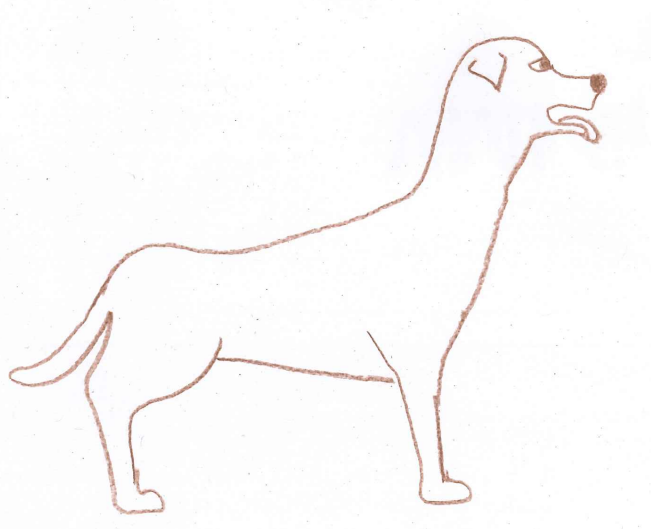
\includegraphics[width=\textwidth]{\dir/dog}
\caption{A two-dimensional dog.}
\label{fig:dog}
\end{subfigure}

\begin{subfigure}[p]{0.45\textwidth}
\centering
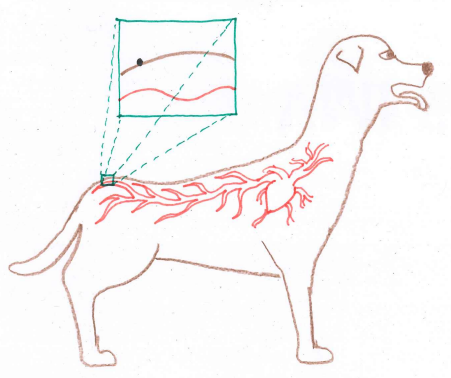
\includegraphics[width=\textwidth]{\dir/dog_close_up}
\caption{A part of the dog's (two-dimensional) cardiovascular system.}
\label{fig:dog_close_up}
\end{subfigure}

\begin{subfigure}[p]{0.45\textwidth}
\centering
        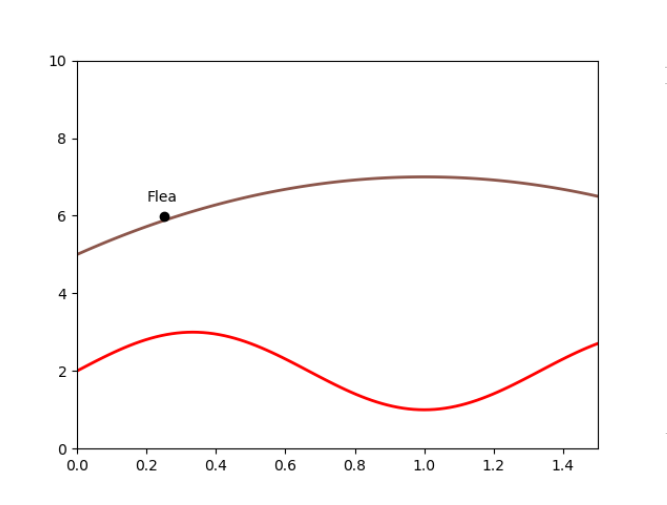
\includegraphics[width=\textwidth]{\dir/vegan_mosquito_start}
        \caption{The flea, the skin, and the upper border of a blood vessel.}
        \label{fig:skin_vessel_simp}
\end{subfigure}
\caption{}
\label{fig:dog_vessel_flea}
\end{figure}

Figure~\ref{fig:skin_vessel_simp} shows the area marked by the green square in detail. We have placed some Cartesian axes there for reference. There is a flea at coordinates (0.25, 6). The dog's skin is the brown curve, and the upper border of a blood vessel is the red curve. Observe that, in a two-dimensional space, skins are lines instead of surfaces.

\subsection{The skin and the blood vessel's upper border}

\newcommand{\skin}{\mathit{skin}}
\newcommand{\vessel}{\mathit{vessel}}

We now mathematically model the skin and the blood vessel's upper border.
Let $\skin : [0, 1] \times \timedomain \to \mathbb{R}$, and $\vessel : [0, 1] \times \timedomain \to \mathbb{R}$ be two functions. For $t \in \timedomain$, let $\skin(\cdot, t) : [0, 1] \to \mathbb{R}$ be the function that maps $x$ to $\skin(x, t)$. We define the function $\vessel(\cdot, t)$ analogously. Intuitively, for $t \in \timedomain$, the functions $\skin(\cdot, t)$ and $\vessel(\cdot, t)$ describe the skin and the blood vessel's upper border at time $t$, as depicted in Figure~\ref{fig:skin_vessel}. Hence, $\skin(x, t) \geq \vessel(x, t)$, for any $(x, t) \in [0, 1] \times \timedomain$. 
%Although the skin surface and the blood vessel should be modeled in $\mathbb{R}^3$, we restrict ourselves to $\mathbb{R}^2$ to keep the presentation simple. 
Observe that $\skin(\cdot, t)$ and $\vessel(\cdot, t)$ vary with $t$. This is to model the fact that blood flows through the vessel and, consequently, makes the skin surface and the blood vessel's upper border vary with time. The animated .gif file attached with these notes\footnote{\url{https://people.inf.ethz.ch/ccarlos/assets/em/vegan\_flea.gif}} illustrate the setting. We strongly encourage the reader to look the .gif file before proceeding.

\begin{figure}
    \centering
    \begin{subfigure}[b]{0.8\textwidth}
        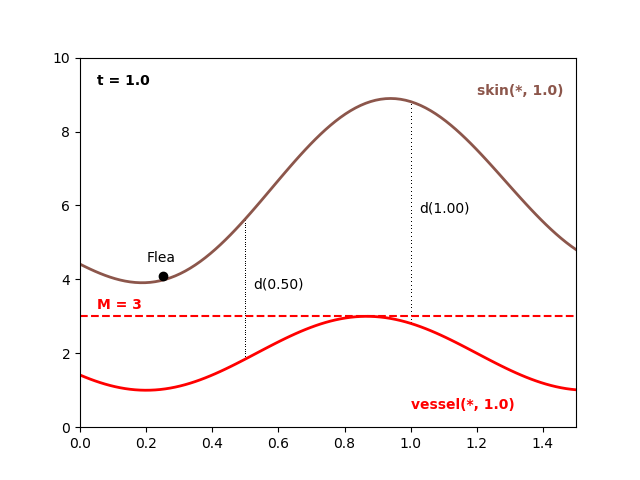
\includegraphics[width=\textwidth]{\dir/vegan_mosquito_40}
        \caption{Skin and blood vessel at $t = 1$}
        \label{fig:skin_vessel_t0}
    \end{subfigure}
    ~ %add desired spacing between images, e. g. ~, \quad, \qquad, \hfill etc. 
      %(or a blank line to force the subfigure onto a new line)
      
    \begin{subfigure}[b]{0.8\textwidth}
        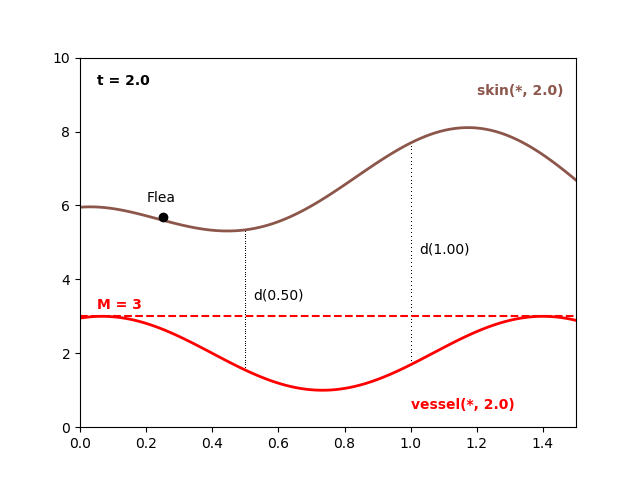
\includegraphics[width=\textwidth]{\dir/vegan_mosquito_80}
        \caption{Skin and blood vessel at $t = 2$}
        \label{fig:skin_vessel_t1}
    \end{subfigure}
    ~ %add desired spacing between images, e. g. ~, \quad, \qquad, \hfill etc. 
    %(or a blank line to force the subfigure onto a new line)
    \caption{An illustration of the functions $\skin(\cdot, t)$ and $\vessel(\cdot, t)$, for $t \in \{1, 2\}$.}\label{fig:skin_vessel}
\end{figure}

\begin{assumption}
We assume that for any $x \in [0, 1]$ and any two time points $t_1, t_2 \in \timedomain$, $\skin(x, t_1) - \vessel(x, t_1) = \skin(x, t_2) - \vessel(x, t_2)$. 
\label{asm:unelastic_skin}
\end{assumption}

This assumption states that the skin surface changes by the same amount that the blood vessel's upper border changes. This allows us to define a function $d$ such that $d(x) = \skin(x, t) - \vessel(x, t)$, for any $x \in [0, 1]$ and $t \in \timedomain$.

Blood flows periodically through the vessel and therefore makes the vessel shape change. Moreover, we assume the following:

\begin{assumption}
For any $x \in [0,1]$ and any $t \in \timedomain$, there is $t' \geq t$ such that $\vessel(x, t') = \max_{x'}\vessel(x', t')$.
\label{asm:periodic_flow}
\end{assumption}

If you observe the .gif animation, you can see that we defined a constant $M$. You can also see that, for any $x$ and any $t$, $\vessel(x, t) \leq M$ and that there is $t' \geq t$ such that $\vessel(x, t') = M$. We could then make Assumption~\ref{asm:periodic_flow} stronger by stating that, for any $x \in [0, 1]$ and any $t \in \timedomain$, $\vessel(\cdot, t)$ is bounded by $M$ and that there is $t' \geq t$ such that $\vessel(x, t) = M$. However, Assumption~\ref{asm:periodic_flow} is enough for our purposes. Moreover, it is weaker and, hence, more general.

\subsection{The vegan flea}

Imagine now that there is a flea resting on the skin surface at $(x_0, \skin(x_0, 0))$, for some $x_0 \in [0, 1]$. The flea has decided to become vegan and wishes to be as far away from the blood vessel as possible, to avoid the temptation of the blood. More precisely, the flea's goal is the following.

\begin{objective}
Compute a value $x^*$ that maximizes $d$.
\end{objective}

A look at the .gif file shows that $x^* = 1.0$. This is easy for us as we, three-dimensional creatures, have an omniscient view of the flea's universe. The flea, however, cannot see that as she knows nothing about $\vessel$. In spite of this, we illustrate how the flea can partially achieve its objective.

We make two assumptions about the flea's computation abilities.

\begin{assumption}
For any $t \in \timedomain$, the flea can efficiently compute 
%
$$x^* = \arg\max_{x'}\skin(x, t).$$
%
\label{asm:flea_m_step}
\end{assumption}

This assumption bases on the idea that the flea can see the dog's skin and can therefore maximize $\skin(\cdot, t)$. The next assumption states that the flea, located at $(x_0, (\skin(x_0, 0)))$, can identify the moment $t'$ when $\vessel(x_0, t') = M$, the maximum of $\vessel(\cdot, t)$. 

\begin{assumption}
For any $x \in [0, 1]$ and any $t \in \timedomain$, the flea can efficiently compute some $\hat{t} \geq t$ such that $\vessel(x, \hat{t}) = \max_{x'}\vessel(x', \hat{t})$.
\label{asm:flea_e_step}
\end{assumption}
%
We give some justification for this assumption. Blood flows through the vessel in a periodic way and $\skin(\cdot, t)$ changes in the same way as $\vessel(\cdot, t)$ does. Hence, the flea can learn the blood pulse and then wait for a time $\hat{t}$ where $\vessel(x_0, \hat{t}) = M$.

\subsection{An approximate maximization algorithm}
\label{sub:approx_max_algo}

We describe a strategy by which the flea can compute a value $x^*$ such that $d(x^*) \geq d(x_0)$, where $(x_0, \skin(x_0, 0))$ is the flea's current position.
%
\begin{description}
\item[[E-step]] The flea waits for a time $\hat{t}$ at which $\vessel(x_0, \hat{t}) = \max_x\vessel(x, \hat{t})$ (Figure~\ref{fig:vegan_flea_opti_s1}). This is possible by Assumption~\ref{asm:flea_e_step}.
\item[[M-step]] At time $\hat{t}$, the flea computes a value $x^*$ such that 
%
$$x^* = \arg\max_{x} \skin(x, \hat{t}).$$
%
(Figure~\ref{fig:vegan_flea_opti_s2}). This is possible by Assumption~\ref{asm:flea_m_step}.
\item[[Move]] The flea moves to $(x^*, \skin(x^*, \hat{t}))$ (Figure~\ref{fig:vegan_flea_opti_s3}). 
\end{description}
%
Figure~\ref{fig:vegan_flea_proof_non_decrease} illustrates why $d(x^*) \geq d(x_0)$. Observe that $\skin(x^*, \hat{t}) \geq \skin(x_0, \hat{t})$, since $x^*$ is a maximum of $\skin(\cdot, \hat{t})$. Observe also that $\vessel(x^*, \hat{t}) \leq \vessel(x_0, \hat{t})$, since $\vessel(x_0, \hat{t})$ is a maximum of $\vessel(\cdot, \hat{t})$. Hence, $d(x^*) = \skin(x^*, \hat{t}) - \vessel(x^*, \hat{t}) \geq \skin(x_0, \hat{t}) - \vessel(x_0, \hat{t}) = d(x_0)$.

\begin{figure}
\centering
\begin{subfigure}[b]{0.6\textwidth}
\centering
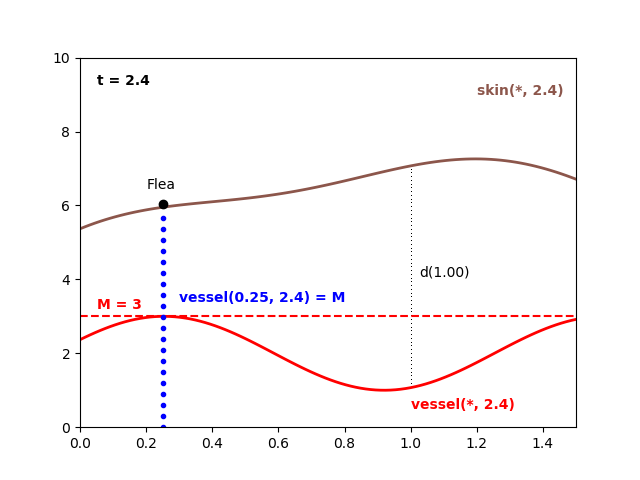
\includegraphics[width=\textwidth]{\dir/vegan_mosquito_e_step}
\caption{Step 1.}
\label{fig:vegan_flea_opti_s1}
\end{subfigure}

\begin{subfigure}[p]{0.6\textwidth}
\centering
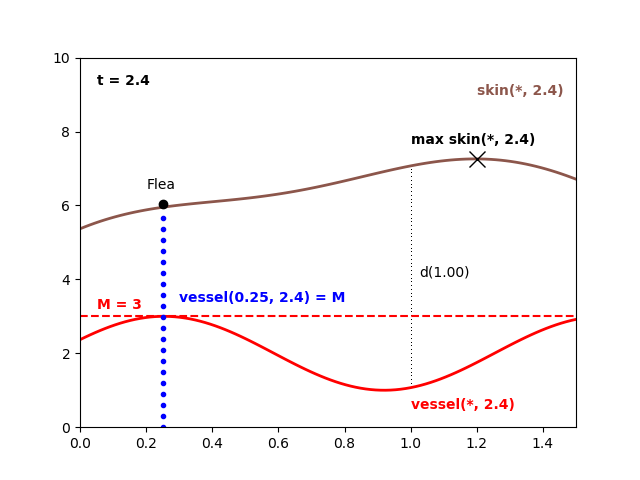
\includegraphics[width=\textwidth]{\dir/vegan_mosquito_m_step_before_jump}
\caption{Step 2.}
\label{fig:vegan_flea_opti_s2}
\end{subfigure}

\begin{subfigure}[p]{0.6\textwidth}
\centering
        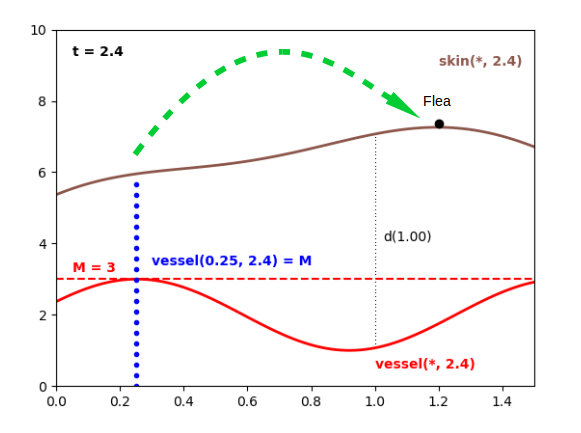
\includegraphics[width=\textwidth]{\dir/vegan_mosquito_m_step_after_jump}
        \caption{Step 3.}
        \label{fig:vegan_flea_opti_s3}
\end{subfigure}
\caption{}
\label{fig:vegan_flea_opti_algo}
\end{figure}

\begin{figure}
\centering
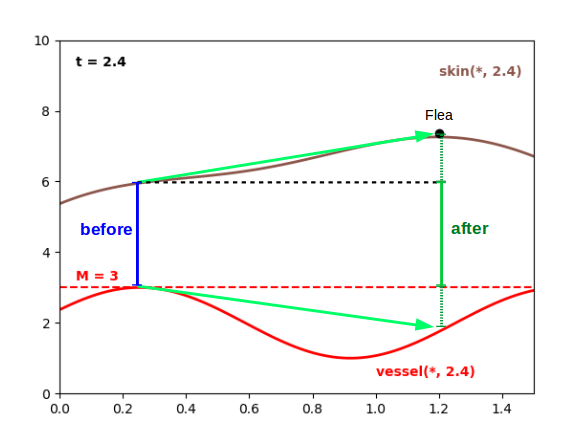
\includegraphics[width=0.6\textwidth]{\dir/vegan_mosquito_proof_nondecrease}
\caption{}
\label{fig:vegan_flea_proof_non_decrease}
\end{figure}

Notice that the flea can set $x_0 = x^*$ and repeat this procedure to find another value $x^{**}$ such that $d(x^{**}) \geq d(x^*)$. The flea can repeat this process as long as the computed values increase $d$. 

We summarize these insights into Algorithm~\ref{algo:vegan_flea}, which computes a sequence of values $x_0$, $x_1, \ldots$ such that $d(x_0) \leq$ $d(x_1) \leq \ldots$ Observe that this algorithm converges. 

One can also relax the assumptions above so that the algorithm works even when $\vessel$ and $\skin$'s domains are a product $\mathcal{X} \times \mathcal{T}$ of any two sets $\mathcal{X}$ and $\mathcal{T}$.

\begin{algorithm}[h!]
\caption{}
\label{algo:vegan_flea}
\begin{algorithmic}[1]
\Require{$\mathcal{X}$ and $\mathcal{T}$ two sets and real functions $d$, $\vessel$, and $\skin$ satisfying the following.
\begin{description}
\item[A1]\label{asm:gen_dist_indep_time} $d(x) = \skin(x, t) - \vessel(x, t)$, for any $x \in \mathcal{X}$ and $t \in \mathcal{T}$.
\item[A2]\label{asm:gen_e_asm} For any $x \in \mathcal{X}$, one can efficiently compute $\hat{t} \in \mathcal{T}$ such that $\vessel(x, \hat{t}) = \max_{x'}\vessel(x', \hat{t})$.
\item[A3]\label{asm:gen_m_asm} For any $t \in \mathcal{T}$, one can efficiently compute $\arg\max_x \skin(x, t)$. 
\end{description}}
\Function{DistanceMax}{$\vessel : \mathcal{X} \times \mathcal{T} \to \mathbb{R}$, $\skin : \mathcal{X} \times \mathcal{T} \to \mathbb{R}$}
	\State {Choose any $x_0 \in \mathcal{X}$.}
	\For {$i = 0, 1, \ldots$}
		\State {\textbf{[E-step]} Compute $\hat{t} \in \mathcal{T}$ s.t. $\vessel(x_0, \hat{t}) = \max_x\vessel(x, \hat{t})$.}
		\State {\textbf{[M-step]} Compute $x^* = \arg\max_x \skin(x, \hat{t})$.}
		\State Print $x^*$ and $d(x^*)$.
		\State $x_0 \gets x^*$.
	\EndFor
\EndFunction
\end{algorithmic}
\end{algorithm}
%

With an argumentation similar to the one above, one can prove that $d(x^*)$ never decreases between two iterations of Algorithm~\ref{algo:vegan_flea}'s loop.

\section{Building a movie-recommendation system with a mixture of multivariate Bernoulli distributions}
\label{sec:movie_recommendation}

\begin{table}[hbtp]
  \begin{tabulary}{\textwidth}{|r|C|C|c|C|C|C|}
\hline
& Star Wars & Star Trek & Titanic & Pretty Woman & 007 & Mission Impossible\\
\hline
\hline
Alice & $\checkmark$ & $\checkmark$ & $\times$ & $\times$ & $\times$ & $\times$ \\
\hline
Bob & $\checkmark$ & $\checkmark$ & $\times$ & $\times$ & $\times$ & $\times$ \\
\hline
Carlos & $\times$ & $\times$ & $\checkmark$ & $\checkmark$ & $\times$ & $\times$\\
\hline
David & $\times$ & $\times$ & $\checkmark$ & $\checkmark$ & $\times$ & $\times$\\
\hline
Ellen & $\times$ & $\times$ & $\checkmark$ & $\times$ & $\times$ & $\checkmark$\\
\hline
Fabian & $\times$ & $\times$ & $\checkmark$ & $\checkmark$ & $\times$ & $\times$\\
\hline
Gabriel & $\checkmark$ & $\checkmark$ & $\times$ & $\times$ & $\checkmark$ & $\checkmark$ \\
\hline
Hector & $\checkmark$ & $\times$ & $\times$ & $\times$ & $\checkmark$ & $\checkmark$ \\
\hline
Ian & $\checkmark$ & $\checkmark$ & $\times$ & $\times$ & $\checkmark$ & $\checkmark$ \\
\hline
Zelya & $\checkmark$ & $\times$ & $\checkmark$ & $\times$ & $\times$ & $\checkmark$ \\
\hline
John & ? & ? & ? & $\checkmark$ & ? & ? \\
\hline

  \end{tabulary}  
    \caption{Ratings from 10 individuals for 6 movies. According to the table, everyone who likes Pretty Woman also liked Titanic. Therefore, it is likely that John would also like Titanic.}
\label{tab:movie_ratings}
\end{table}
%

Table~\ref{tab:movie_ratings} shows the ratings that 10 (fictitious) individuals gave to 6 popular movies. To keep it simple, we assume only binary ratings (good or bad). After a close look to the ratings, the reader can see that Alice and Bob have the exact same taste for movies: \emph{sci-fi} movies. The next four people have a strong interest for \emph{romantic} movies. The next three people like sci-fi and action movies. Zelya's tastes seem to be different from everyone else.

Consider now John, he likes Pretty Woman, but does not like Star trek. He has not seen any of the other movies. What movie could we recommend to him? Since he likes Pretty Woman and everyone who liked Pretty Woman also liked Titanic, we can recommend him to watch Titanic.

From all $2^6$ combinations of ratings, the table contains only a few of them. Moreover, a large majority of the people in the table seem to belong to one of very few taste categories: sci-fi, romantic, or sci-fi+action. Real life is not so different: a large majority of people can partitioned into very few categories and people within a same category have very similar preferences. To recommend a movie to someone, we estimate the category where this person belongs and then search for a movie that people in this category liked.\looseness=-1

\subsection{Movie ratings as samples from probability distributions}
\label{sub:ratings_as_samples}

We can view Table~\ref{tab:movie_ratings} as the result of a sampling process. Initially, the table was empty and then one person at random appeared (Alice, in our case) and filled the first row of the table. Then Bob appeared and so on. To sample the film ratings of one person, we first \emph{sample the category} where this person belongs and then, for each movie, we \emph{sample the rating} this person gave to that movie, conditioned on the person belonging to the sampled category. This sampling process is then defined by the following probability distributions:

\begin{itemize}
\item A distribution over categories.
\item For each category and each movie, a distribution defining the probability that a person in the category likes the movie.
\end{itemize}

From these two distributions, we build a new probability distribution with which we can answer the following question: \emph{if a person watched and liked movies $m_1$, $m_2, \ldots$, and $m_k$, how likely is that she will like a movie $m'$ that she has not seen?} This probability distribution constitutes then our recommendation system. To decide which movie to recommend, we take the ratings the person has given to previously watched movies. Then, for each movie in the database she has not seen, we compute the probability that she likes that movie. Finally, we recommend the movie that she will most likely like.

We first formalize the two distributions mentioned above. Suppose we have $K$ categories and $D$ movies. We identify categories with the numbers $1$, $2, \ldots$, $K$ and movies with the numbers $1$, $2, \ldots$, $D$. We can model the distribution of $K$ categories using a discrete distribution with a set $\{\nu_1$, $\nu_2, \ldots$, $\nu_{K}\}$ of $K$ parameters that add up to 1. For the $k$-th category and the movie $j$, we define a value $\mu_{kj}$ indicating what the probability is that a person in the $k$-th category likes movie $j$. We leave the values $\nu_k$ and $\mu_{kj}$, for $k \leq K$ and $j \leq D$, undefined for the moment.

Having defined these distributions, we can now assign a probability to the ratings a person gave to all movies in the database. We model these ratings with a vector $x \in \{0, 1\}^D$, where $x_j$, for $j \leq D$, indicates whether the movie was rated good ($x_j = 1$) or bad ($x_j = 0$). We leave as an exercise to show that the probability $p(x)$ of a vector $x \in \{0, 1\}^D$ is as follows:
%
\begin{equation}
p(x) = \sum_{k \leq K} \left(\nu_k \prod_{j \leq D} \mu_{kj}^{x_j}\left(1 - \mu_{kj}\right)^{1 - x_j}\right).
\label{eq:individual_likelihood}
\end{equation}
%
We can now define probabilities for movie-rating databases. We model a movie-rating database with a matrix $X \in \{0, 1\}^{N \times D}$. Each row $X_i$, for $i \leq N$, represents a person and each entry $X_{i,j}$, for $j \leq D$, represents the rating person $i$ gave to movie $j$. Assuming that the ratings of two different people are independent, we can show that the probability $p(X)$ is given by the following.
%
\begin{equation}
p(X) = \prod_{i \leq N} p(X_i) = \prod_{i \leq N} \sum_{k \leq K} \left(\nu_k \prod_{j \leq D} \mu_{kj}^{X_{i,j}}\left(1 - \mu_{kj}\right)^{1 - X_{i,j}}\right).
\label{eq:incomplete_likelihood}
\end{equation}
%

\subsection{Maximum-likelihood estimation}

We now choose values for $\nu_k$ and $\mu_{kj}$, for $k \leq K$ and $j \leq D$. Here, we use \emph{maximum-likelihood estimation}, which argues that the best values for our parameters are those that maximize $p(X)$, for $X$ the movie database we have. For computational reasons, one searches instead for the parameters that maximize $\log p(X)$. Using basic logarithm properties, we can show that
%
%
\begin{equation}
\log p(X) = \sum_{i \leq N} \log \left(\sum_{k \leq K} \left(\nu_k \prod_{j \leq D} \mu_{kj}^{x_j}\left(1 - \mu_{kj}\right)^{1 - x_j}\right)\right).
\label{eq:log_incomplete_likelihood}
\end{equation}
%
%
The value $\log p(X)$ is called \emph{$X$'s log likelihood}. 

Finding the parameter values that maximize this log likelihood is difficult, even with approximation methods. Nonetheless, it is possible to find a set of parameter values that locally maximize the log likelihood, using Algorithm~\ref{algo:vegan_flea}. To do this, we introduce a new set $\mathbf{Z} = \{\mathbf{Z}(i) \mid i \leq N\}$ of random variables. For $i \leq N$, $\mathbf{Z}(i)$ indicates to which category person $i$ belongs. Assume for a moment that, in addition of $X$, we also know, for $i \leq N$, the category $Z(i)$ where person $i$ belongs. One can show that $(X, Z)$'s log likelihood is given by the following.
%
\begin{equation}
\log p(X, Z) = \sum_{i \leq N} \left( 
\begin{array}{l}
\log \nu_{Z(i)} + \\ 
x_{i,Z(i)}\log {\mu_{Z(i), j}} + \\
\left(1 - x_{i, Z(i)}\right)\log \left(1 - \mu_{Z(i),j}\right)
\end{array}\right).
\label{eq:log_complete_likelihood}
\end{equation}
%
The log likelihood of $(X, Z)$ is much easier to maximize with respect to the parameters than $X$'s log likelihood; it can be maximized using standard calculus. However, observe that the movie database does not tell us to which category each person belongs, so we do not know $Z$ and there is no clear way how to obtain it.

It is common that log likelihood maximization problems become easier when we introduce additional random variables to the probabilistic model. It is also common that the values that such random variables take are not available. For these situations, the EM-algorithm was proposed.

\section{Derivation of the EM-algorithm}
\label{sec:em_algo}

We generalize the problem we addressed in the previous section. Let $\mathbf{X}$ and $\mathbf{Z}$ be random variables and let $X$ be an observed value for $\mathbf{X}$. Assume that the joint pdf $p(\cdot, \cdot \mid \theta)$ for $(\mathbf{X}, \mathbf{Z})$ is parameterized by $\theta$, which can take values in $\Theta$. Our goal is to compute
%
\begin{equation}
\arg\max_{\theta \in \Theta} \log p(X \mid \theta).
\label{eq:max_likelihood}
\end{equation}
%
Assume now that it is preferrable to work with $\log p\left(X, Z\right)$ than with $\log p(X)$, for any $Z$ in $\mathbf{Z}$'s range. If we knew the value $Z$ that $\mathbf{Z}$ took when we obtained $\mathbf{X} = X$, then we could state that
%
\begin{equation}
\log p(X \mid \theta) = \log p(X, Z \mid \theta) - \log p (Z \mid X, \theta).
\label{eq:connect}
\end{equation}
%
This identity follows from the definition of conditional pdfs. We can make $Z$ irrelevant by computing expectations on both sides with respect to some pdf $\tilde{p}$ for $\mathbf{Z}$. We leave for later the problem of defining $\tilde{p}$.
%
\begin{align*}
\int \tilde{p}(Z) \log p(X \mid \theta) dZ &= \int \tilde{p}(Z)\log p(X, Z \mid \theta) dZ - \int \tilde{p}(Z)\log p (Z \mid X, \theta) dZ\\[5pt]
&= \mathbb{E}_{\tilde{p}\left(\mathbf{Z}\right)}\left[\log p(X, \mathbf{Z} \mid \theta)\right] - \mathbb{E}_{\tilde{p}\left(\mathbf{Z}\right)}\left[\log p (\mathbf{Z} \mid X, \theta)\right].
\label{eq:log_connect} 
\end{align*}
%

Observe that $\log p(X \mid \theta)$ does not depend on $Z$ or $\tilde{p}$. Therefore, the left-hand side equals $\log p(X \mid \theta)$. As a result,
%
\begin{equation}
\log p(X \mid \theta) = \mathbb{E}_{\tilde{p}\left(\mathbf{Z}\right)}\left[\log p(X, \mathbf{Z} \mid \theta)\right] - \mathbb{E}_{\tilde{p}\left(\mathbf{Z}\right)}\left[\log p (\mathbf{Z} \mid X, \theta)\right].
\label{eq:log_expec_connect} 
\end{equation}
%
We now show that the maximization problem in Equation~\ref{eq:max_likelihood} is an instance of the vegan-flea problem. Let $\mathcal{X} = \Theta$ and $\mathcal{T}$ be the set of all pdfs for $\mathbf{Z}$. For $\theta \in \Theta$ and $\tilde{p} \in \mathcal{T}$, let 
%
\begin{align*}
d(\theta) &= \log p(X \mid \theta)\\
\skin(\theta, \tilde{p}) &= \mathbb{E}_{\tilde{p}\left(\mathbf{Z}\right)}\left[\log p(X, \mathbf{Z} \mid \theta)\right]\\
\vessel(\theta, \tilde{p}) &= \mathbb{E}_{\tilde{p}\left(\mathbf{Z}\right)}\left[\log p (\mathbf{Z} \mid X, \theta)\right].
\end{align*}

We now derive sufficient conditions for the assumptions \textbf{[A1]}, \textbf{[A2]}, and \textbf{[A3]} to hold. 
%
\begin{description}
\item[A1] This assumption follows from Equation~\ref{eq:log_expec_connect}, so no condition is necessary.

\item[A2] In our case, this assumption means the following: for any $\theta \in \Theta$, one can efficiently compute $\tilde{p} \in \mathcal{T}$ such that for any $\theta' \in \Theta$, 
%
\begin{equation}
\mathbb{E}_{\tilde{p}\left(\mathbf{Z}\right)}\left[\log p(\mathbf{Z} \mid X, \theta)\right] \geq \mathbb{E}_{\tilde{p}\left(\mathbf{Z}\right)}\left[\log p(\mathbf{Z} \mid X, \theta')\right].
\label{eq:e_step_req_instan}
\end{equation}
%
We can fulfill this inequality by setting $\tilde{p}\left(\mathbf{Z}\right) = p(\mathbf{Z} \mid X, \theta)$. This follows from Gibbs's inequality, which states that for any two pdfs $p$ and $q$ for a random variable $\mathbf{Z}$,\looseness=-1
%
\begin{equation}
\mathbb{E}_{p\left(\mathbf{Z}\right)}\left[\log p(\mathbf{Z})\right] \geq \mathbb{E}_{p\left(\mathbf{Z}\right)}\left[\log q(\mathbf{Z})\right].
\label{eq:gibbs_inequality}
\end{equation}
%
Hence, for \textbf{[A2]} to hold, we require the pdf $p(\mathbf{Z} \mid X, \theta)$ \emph{to be efficiently computable}.

\item[A3] This assumption requires that, for any $\tilde{p} \in \mathcal{T}$, we can efficiently compute
%
$$\arg\max_{\theta \in \Theta} \mathbb{E}_{\tilde{p}\left(\mathbf{Z}\right)}\left[\log p(X, \mathbf{Z} \mid \theta)\right].$$
%
\end{description}

In summary, to apply Algorithm~\ref{algo:vegan_flea} to compute $\arg\max_\theta \log p\left(X \mid \theta\right)$, we require the following.

\begin{description}
\item[AE1] One can efficiently compute the pdf $p(\mathbf{Z} \mid X, \theta)$.
\item[AE2] One can efficiently compute 
%
$\arg\max_{\theta \in \Theta} \mathbb{E}_{\tilde{p}\left(\mathbf{Z}\right)}\left[\log p(X, \mathbf{Z} \mid \theta)\right],$
%
for any pdf $\tilde{p}$ for $\mathbf{Z}$.
\end{description}

Instantiating Algorithm~\ref{algo:vegan_flea} to our particular problem, we obtain \emph{the EM algorithm}.

\begin{algorithm}[h!]
\caption{}
\label{algo:em_algo}
\begin{algorithmic}[1]
\Require{\text{ }\begin{itemize}
\item $\Theta$ a set of parameters.
\item A joint pdf $p(\mathbf{X}, \mathbf{Z} \mid \theta)$ over two random variables $\mathbf{X}$ and $\mathbf{Z}$, governed by a parameter $\theta$ that ranges over $\Theta$.
\item A value $X$ in $\mathbf{X}$'s range.
\end{itemize}}
\begin{description}
\item[AE1] One can efficiently compute the pdf $p(\mathbf{Z} \mid X, \theta)$.
\item[AE2] One can efficiently compute $\arg\max_{\theta \in \Theta} \mathbb{E}_{\tilde{p}\left(\mathbf{Z}\right)}\left[\log p(X, \mathbf{Z} \mid \theta)\right],$ for any pdf $\tilde{p}$ for $\mathbf{Z}$.
\end{description}
\Function{EM}{$X$, $p(\mathbf{X}, \mathbf{Z} \mid \theta)$, $\Theta$}
	\State {Choose any $\theta_0 \in \Theta$.}
	\For {$i = 0, 1, \ldots$}
		\State {\textbf{[E-step]} Compute $p(\mathbf{Z} \mid X, \theta_{i})$.}
		\State {\textbf{[M-step]} Compute $\theta_{i + 1} = \arg\max_\theta \mathbb{E}_{p(\mathbf{Z} \mid X, \theta_{i})}\left[\log p(X, \mathbf{Z} \mid \theta)\right].$}
		\State Print $\theta_{i+1}$ and $\log p (X \mid \theta_{i+1})$.
	\EndFor
\EndFunction
\end{algorithmic}
\end{algorithm}

\end{document}

https://www.graphsketch.com/?eqn1_color=1&eqn1_eqn=&eqn2_color=2&eqn2_eqn=3%20%2B%20sin(((1*pi)%2F5)*x%20-%206.2)&eqn3_color=3&eqn3_eqn=&eqn4_color=4&eqn4_eqn=10%20%2B%20sin(((2*pi)%2F5)*x%20-%20(2%20*pi)%2F5%20-%200.25)&eqn5_color=5&eqn5_eqn=&eqn6_color=6&eqn6_eqn=&x_min=-1&x_max=15&y_min=-1&y_max=15&x_tick=1&y_tick=1&x_label_freq=5&y_label_freq=5&do_grid=0&do_grid=1&bold_labeled_lines=0&bold_labeled_lines=1&line_width=4&image_w=850&image_h=525

\end{document}
This is never printed
